The unfolding procedure is exactly the same as in Ref.~\cite{cmsSMPJSVJ}. Here we discuss the unfolding
briefly for completeness. 

\subsection{Unfolding}
The measured spectrum of a physical observable, like the jet mass distribution, is usually distorted by	detector effects, such as finite resolution and limited acceptance. Moreover, in this analysis the chosen bin size is comparabl
e to the resolution, so there is a significant migration of events generated in one jet bin mass and ending up in a different bin of reconstructed jet mass. A comparison of the measured mass spectrum with that predicted at generato
r level requires that we remove these effects to obtain the true underlying mass spectrum. There are several possible ways to achieve the unfolding of detector effects on measured spectra, and examples can be found in \cite{unfold}
 and references therein. In this section we describe the unfolding method adopted in this analysis, which largely follows the technique proposed in \cite{agostini}. 
A physical quantity $\alpha$, distributed according to its probability density function $f(\alpha)$, cannot be measured perfectly. Apart from statistical uncertainties, there will be effects from reconstruction efficiency and finite 
resolution of the detector. As	a result, instead of the true, physical variable $\alpha$, 
a variable $\beta$, distributed according to some distribution $g(\beta)$, is measured. 
The relation between $f(\alpha)$ and $g(\beta)$ can be expressed as a convolution of the 
true distribution $f(\alpha)$ with a kernel $\hat{A}(\alpha,\beta)$ describing the detector effects,

\begin{equation}
\int f(\alpha) \hat{A}(\alpha,\beta)d\alpha = g(\beta)
\end{equation}

\noindent The spectrum we intend to unfold is given as an histogram. Hence, we use vectors and matrices for the formulation of the convolution,	

\begin{equation}
\hat{A} x = b
\label{eq:unf1}
\end{equation}

\noindent where the $i$-th component of the $n_x$-dimensional vector $x$ and the $n_b$-dimensional vector $b$ contain the number of entries in bin $i$ of the true and the measured distribution, respectively. 
$\hat{A}$ is a $(n_b - n_x)$-dimensional matrix, and contains the detector effects. An event with a true value in bin $j$ might be measured with a value in bin $i$ (i.e. finite resolution) or might not be measured at all. The matri
x element $\hat{A}_{ij}$ represents the probability for an event	 with a true value in bin $x_j$ to be measured with a value in bin $b_i$.
Assuming that the measurement process is well simulated, $\hat{A}$ can be determined on Monte Carlo events by tracking the true and reconstructed values for each event. A well-defined system of linear equations is obtained,

\begin{equation}
\hat{A} x^{ini} = b^{ini}
\end{equation}


\noindent where the index ``ini''denotes the use of Monte Carlo spectra $x^{ini}$ , $b^{ini}$. Technically, the matrix element $\hat{A}_{ij}$ is determined by taking the number of events that fall into bin $j$ of $x^{ini}$ and at t
he same time into bin $i$ of $b^{ini}$, and by dividing this number by the number of events in bin $j$ of $x^{ini}$.

Now that $\hat{A}$ is determined and we have a measured spectrum $b$, one can try to solve Eq.~\ref{eq:unf1} for the true spectrum $x$. However, the apparently easiest way to determine $x$, i.e. applying $x = \hat{A}^{-1}b$, is not
 adequate. Even when $\hat{A}$ can be inverted, statistical fluctuations in the measured spectrum introduce spurious, non-physical oscillations in the solution for $x$. Therefore a more efficient method needs to be applied. 

We use an unfolding procedure described by G.~D.~Agostini in~\cite{agostini}. Repeated application of Bayes theorem is used to invert the response matrix. Regularization is achieved by stopping iterations before reaching the ``true
'' (but wildly fluctuating) inverse. The regularization parameter is just the number of iterations.
 In principle, this has to be tuned to prevent the statistical fluctuations being interpreted as structure in the true distribution, according to the sample statistics and binning. In practice, the results are fairly insensitive to
 the precise setting used and four iterations are usually sufficient.
The training truth is taken as its initial prior, rather than a flat distribution. This should not bias result once we have iterated, but could reach an optimum after fewer iterations.
This implementation takes account of errors on the data sample but not, by default, uncertainties in the response matrix due to finite MC statistics. That calculation can be very slow, and usually the training sample is much larger
 than the data sample.
%RooUnfoldBayes does not normally do smoothing, since this has not been found to be necessary 2
%and can, in principle, bias the distribution. Smoothing can be enabled with an option.

\ifnpas
The {\tt RooUnfold} package~\cite{roounfold} has been used with the {\tt RooUnfoldBayes} class,
with the number of iterations set to four. 
\fi

\subsection{Response matrices}

The detector response matrix for the different jet clustering algorithms are showed in Fig.~\ref{figs:response_QCD_pythia6_z2_plots_nominal_ptall}-\ref{figs:response_QCD_herwigpp_23_plots_nominal_Pruned_ptall}. 
We show the response in the nine nominal $p_T$ bins used for the analysis, for the AK7 jets with the 
following clustering algorithm: ungroomed, pruned, filtered and trimmed.
In the response matrix derivation, the appropriate physical $\pt$ weighting is
used. If one uses the unphysical flat-$\pt$ spectrum, this introduces
unphysical biases in the tails of the jet mass distribution. 



\begin{figure}[htbp]
\centering
\subfigure{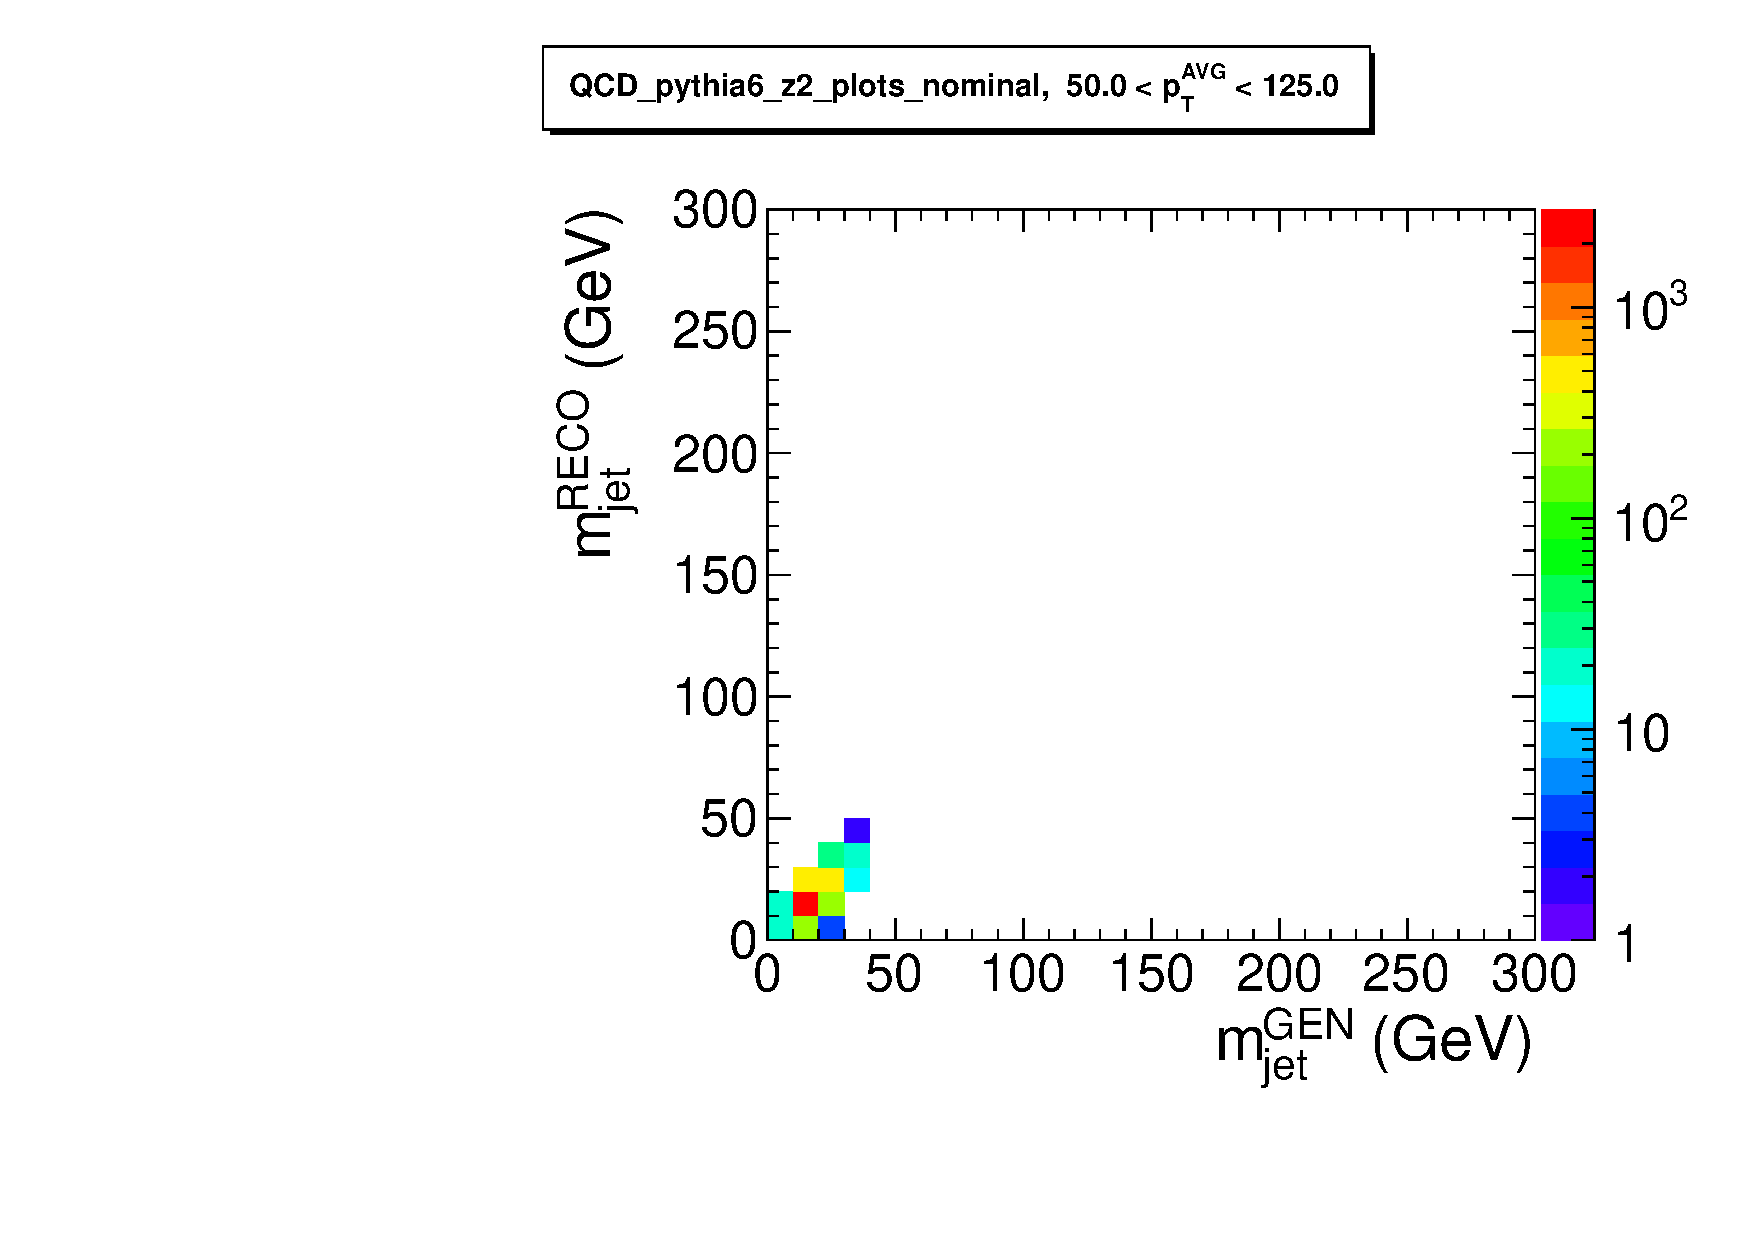
\includegraphics[width=0.3\textwidth]{figs/response_QCD_pythia6_z2_plots_nominal_pt1}}
\subfigure{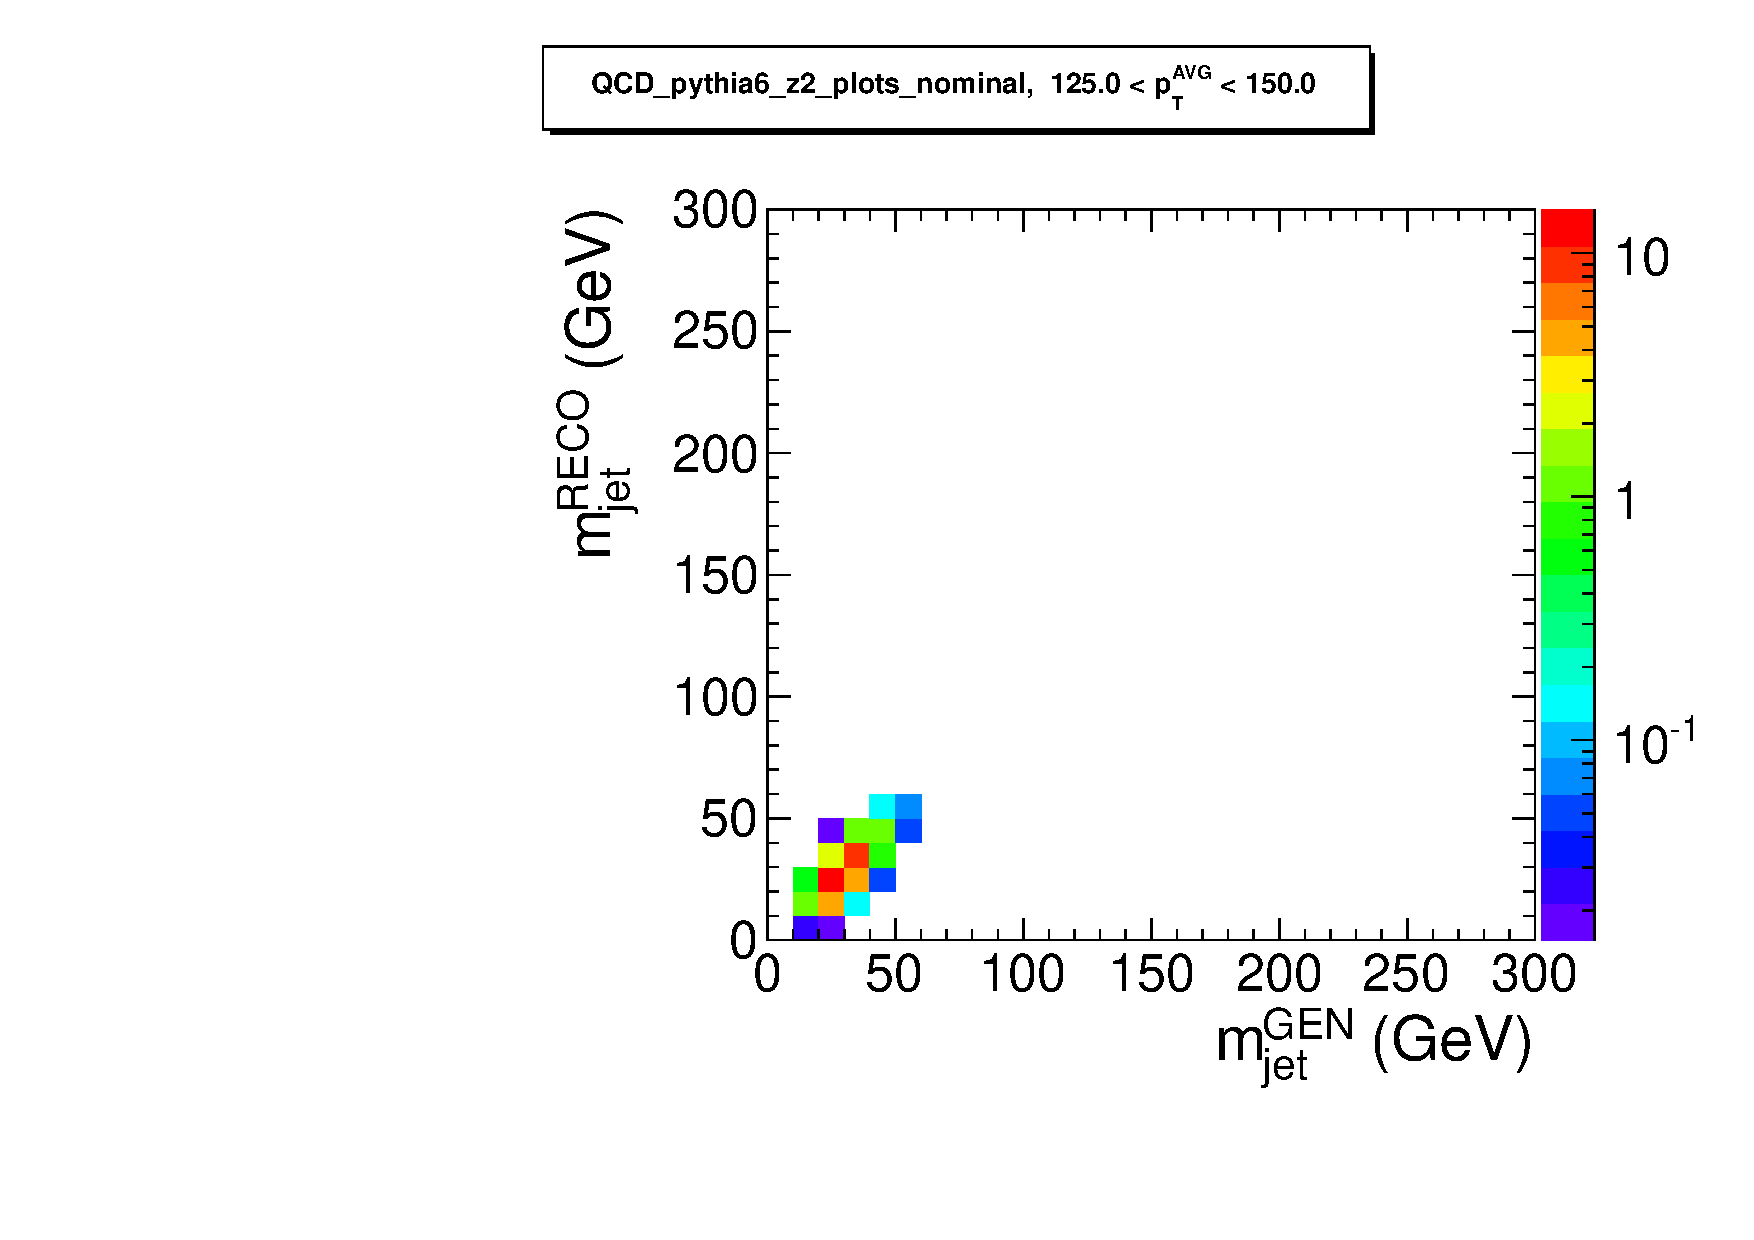
\includegraphics[width=0.3\textwidth]{figs/response_QCD_pythia6_z2_plots_nominal_pt2}}
\subfigure{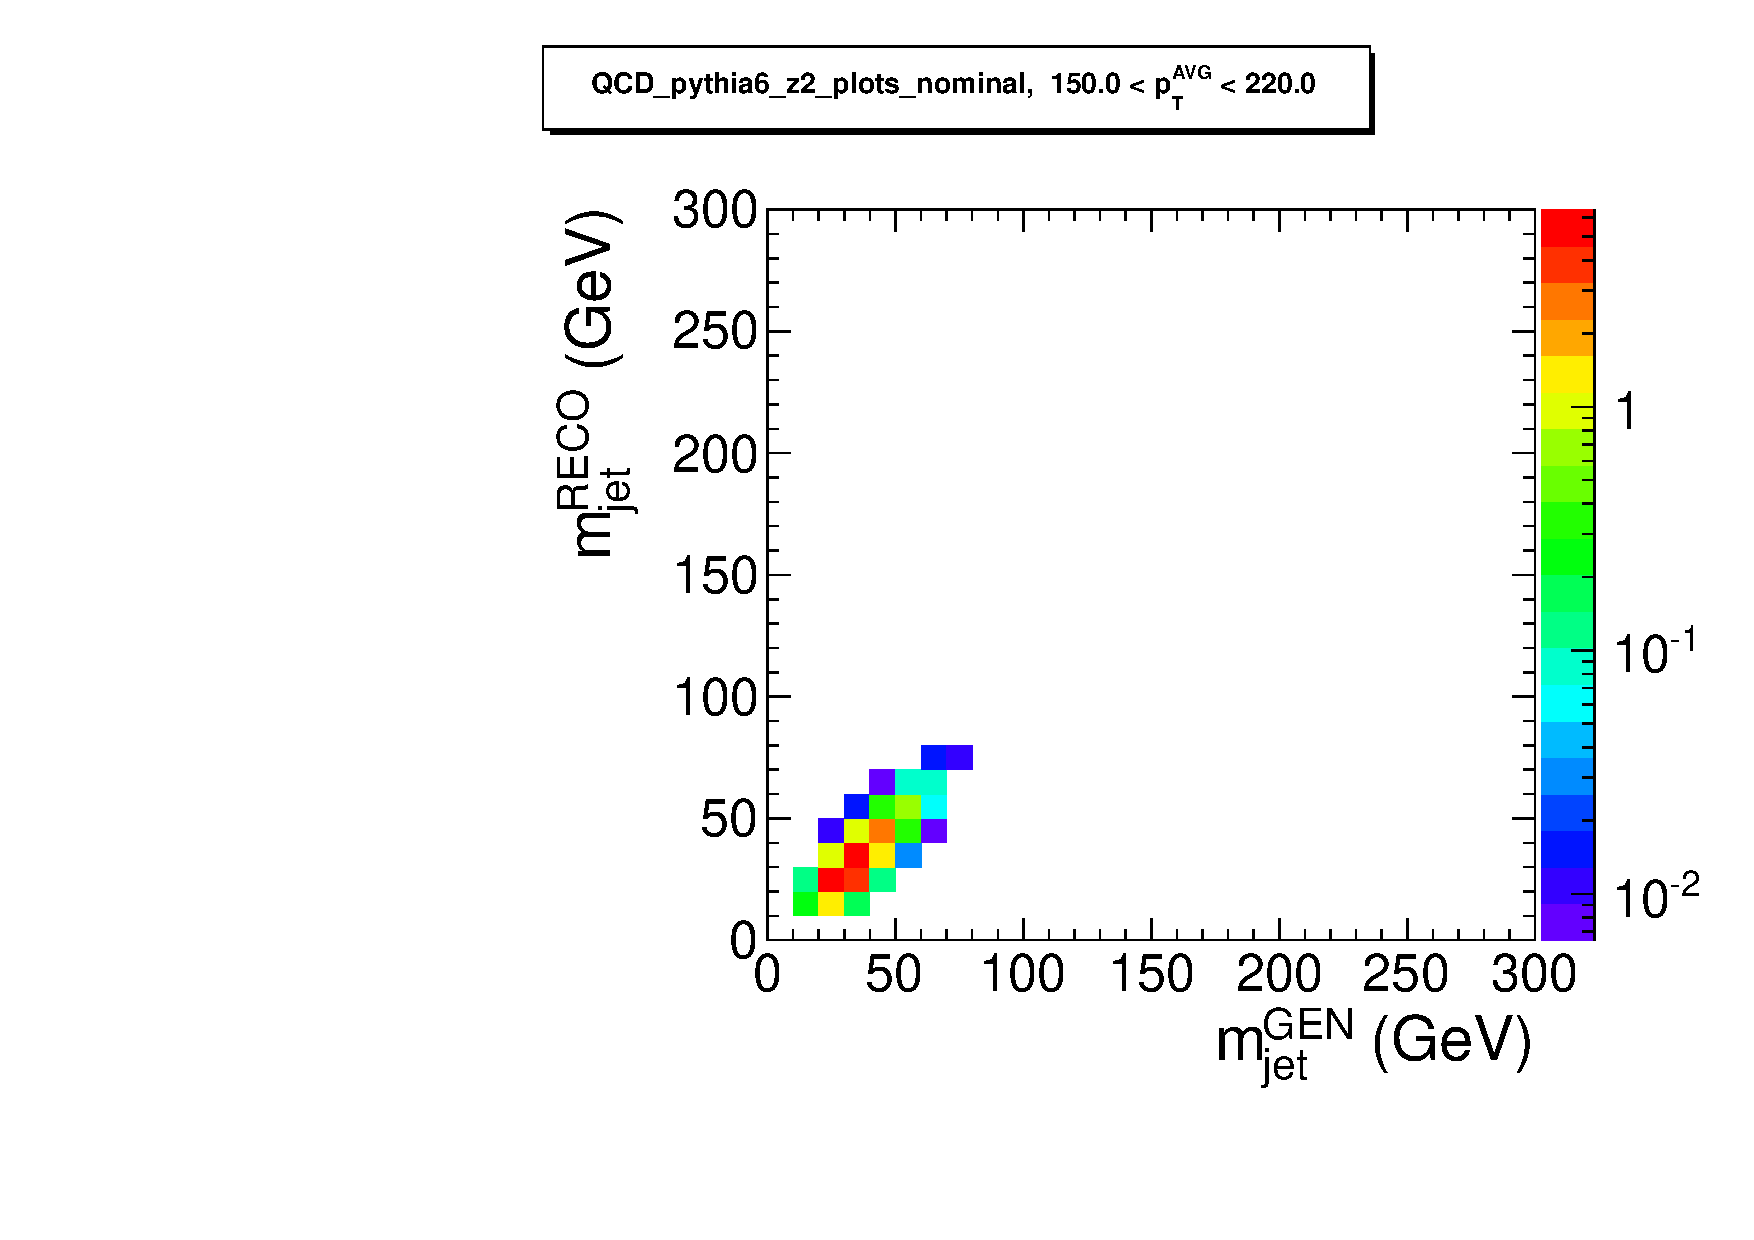
\includegraphics[width=0.3\textwidth]{figs/response_QCD_pythia6_z2_plots_nominal_pt3}}\\
\subfigure{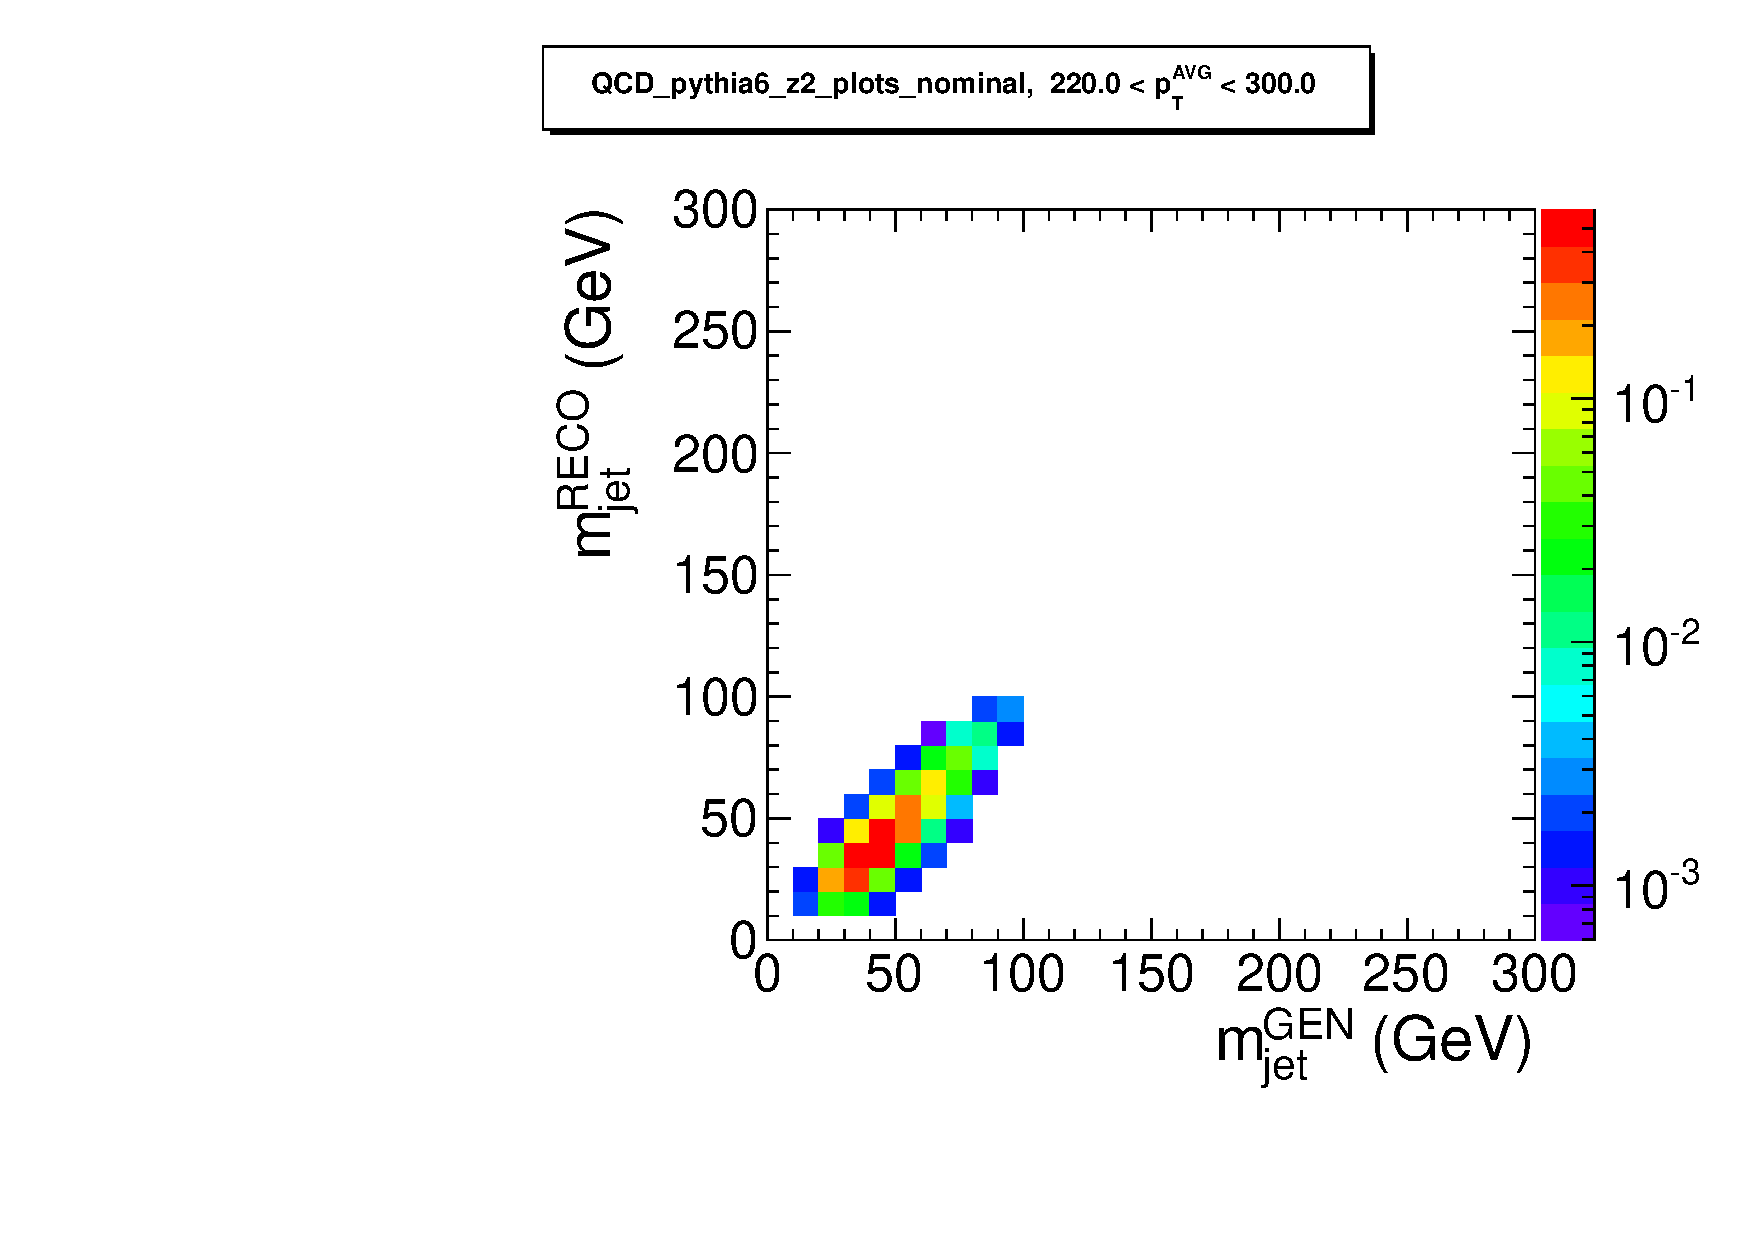
\includegraphics[width=0.3\textwidth]{figs/response_QCD_pythia6_z2_plots_nominal_pt4}}
\subfigure{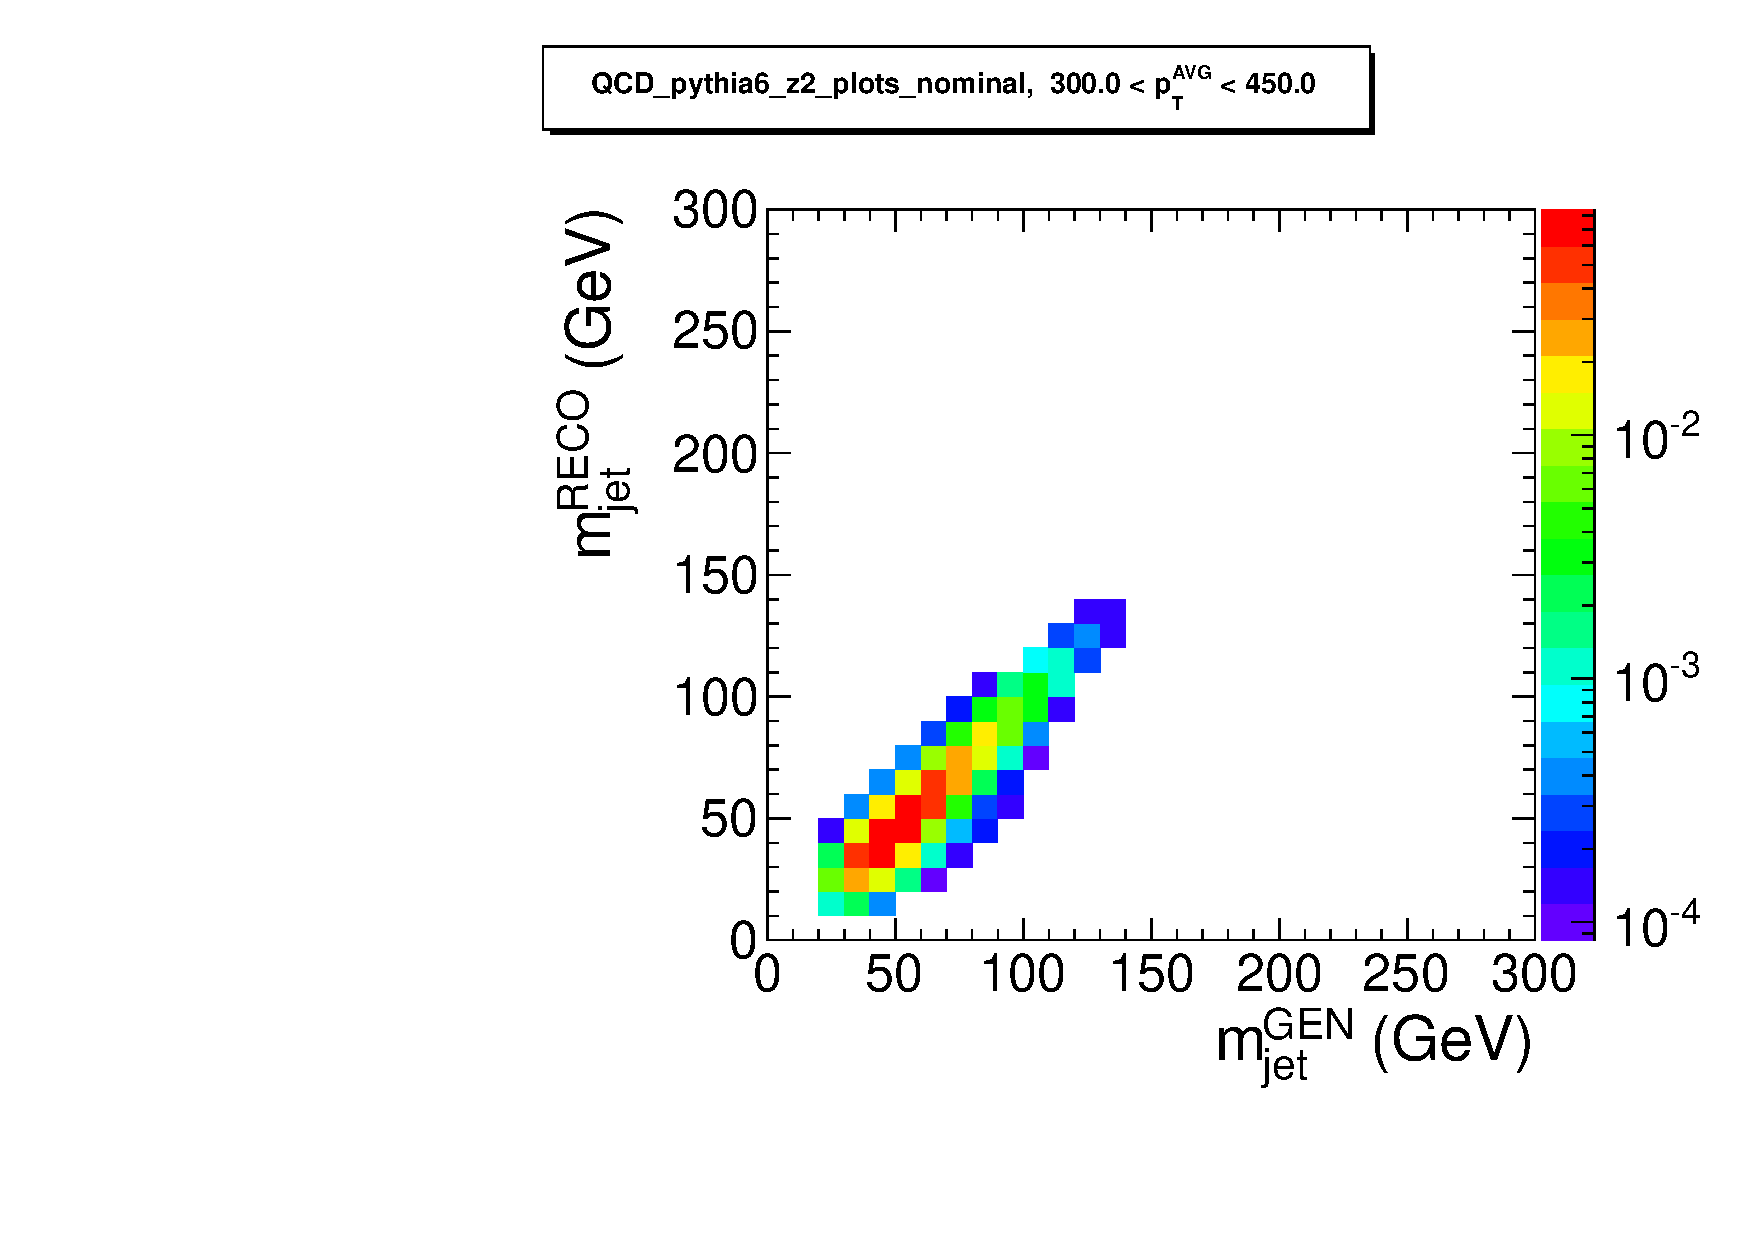
\includegraphics[width=0.3\textwidth]{figs/response_QCD_pythia6_z2_plots_nominal_pt5}}
\subfigure{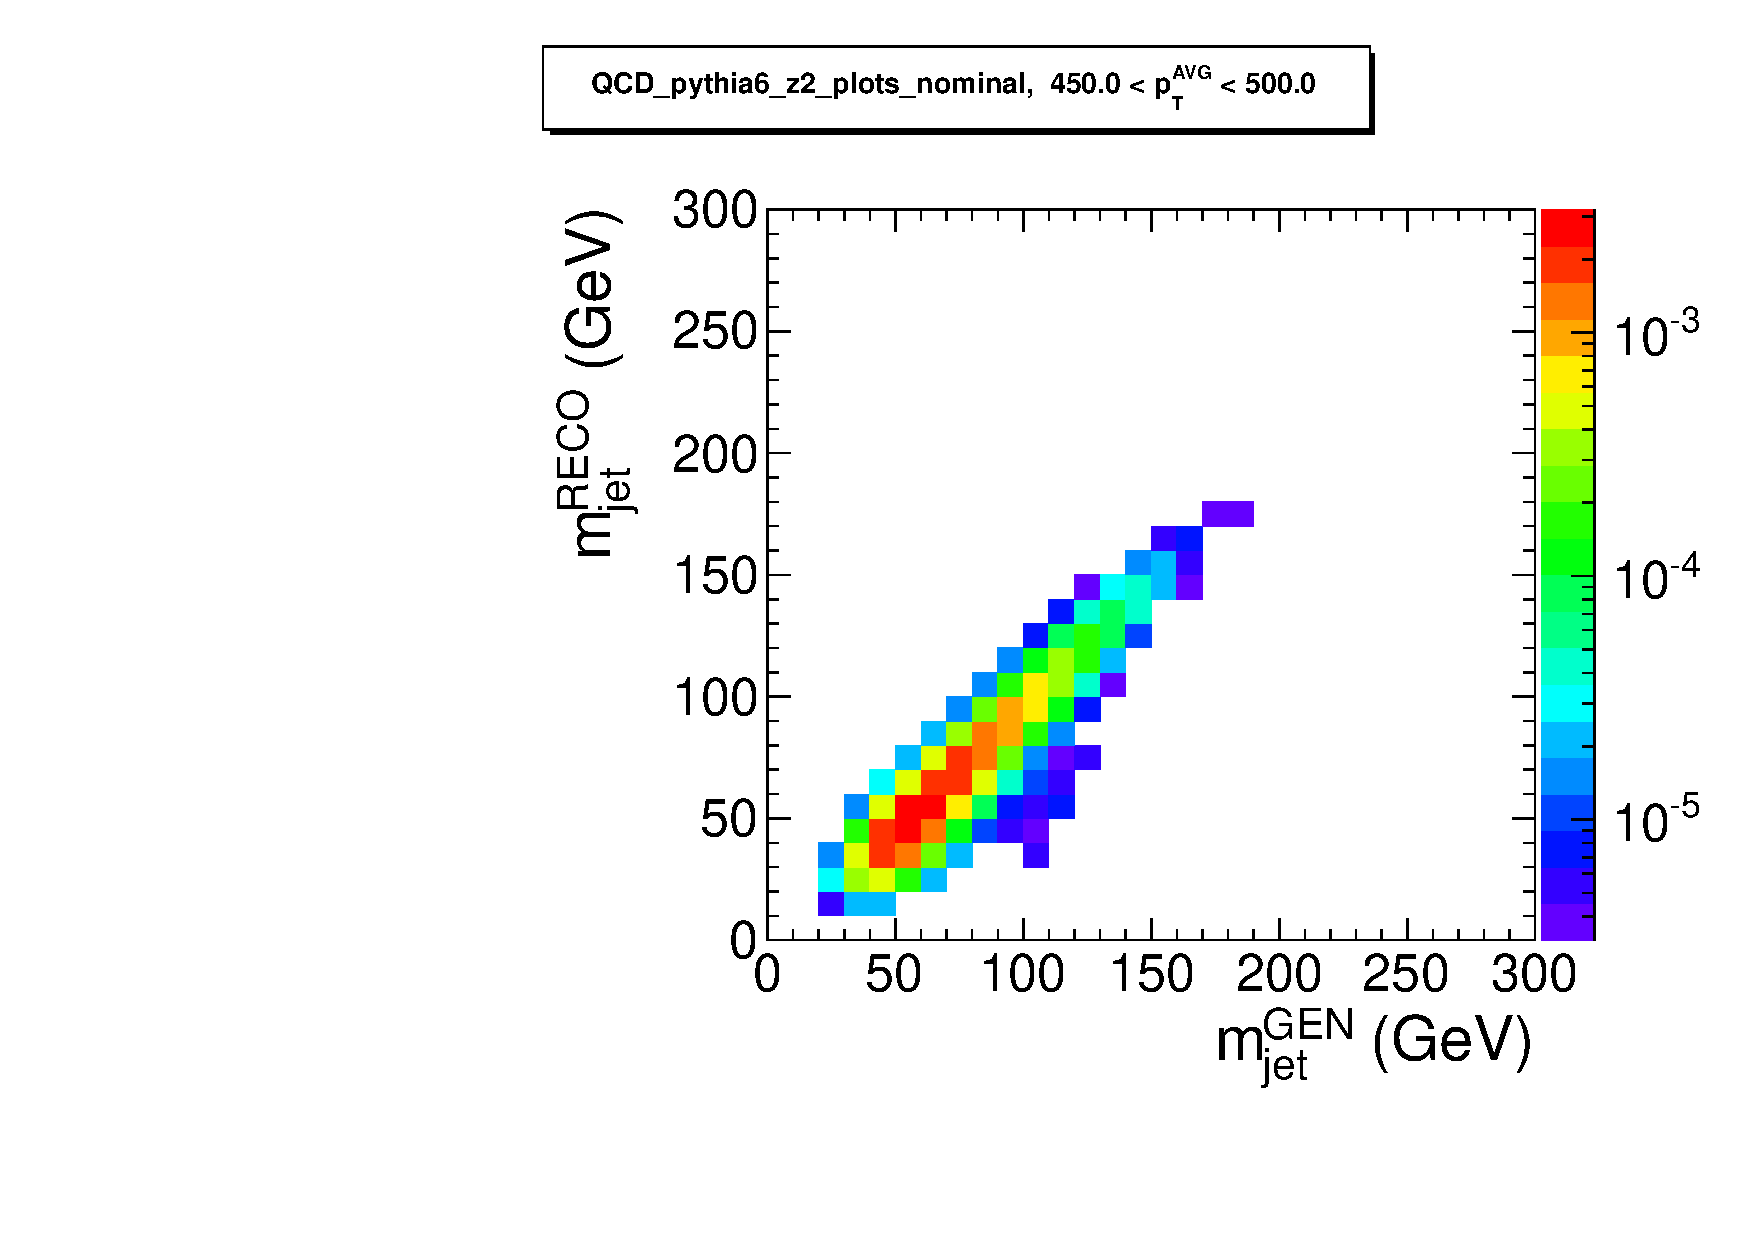
\includegraphics[width=0.3\textwidth]{figs/response_QCD_pythia6_z2_plots_nominal_pt6}}\\
\subfigure{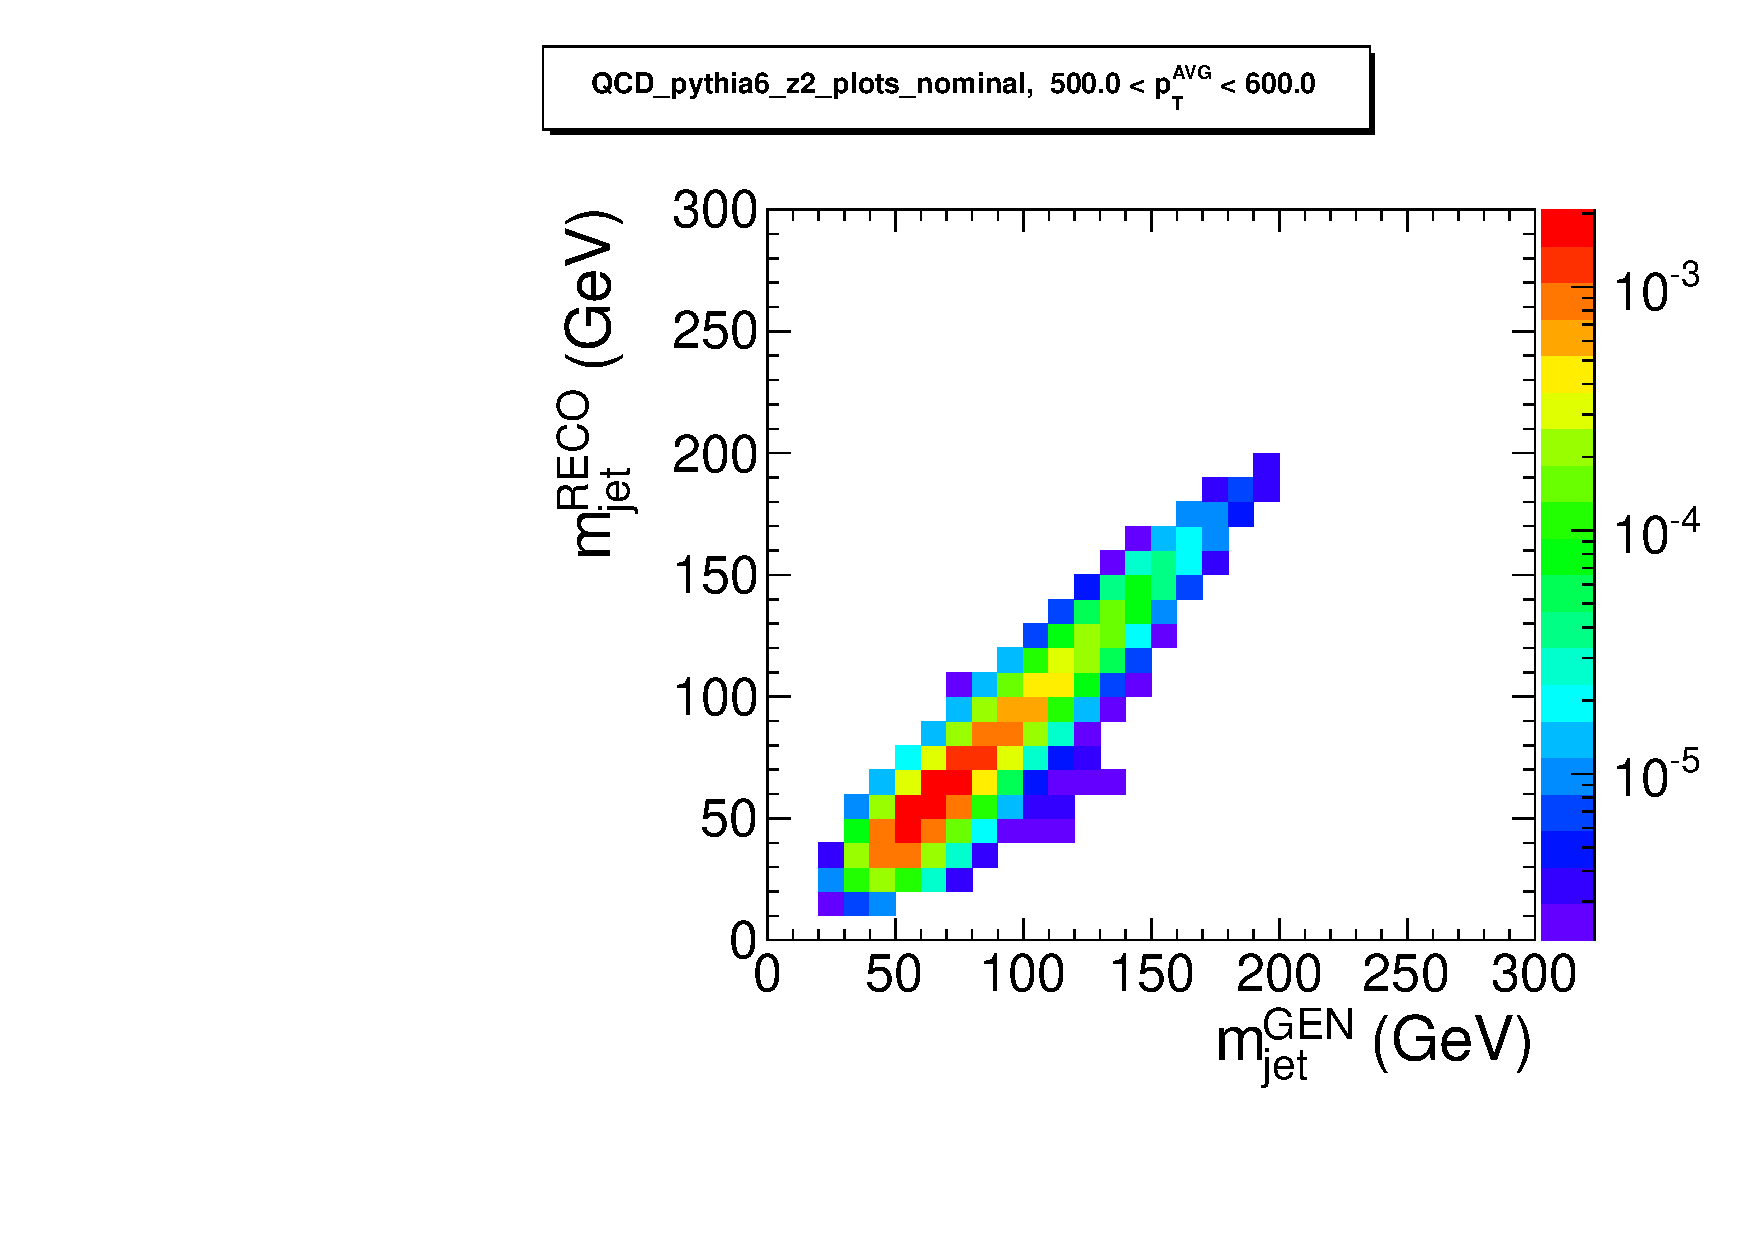
\includegraphics[width=0.3\textwidth]{figs/response_QCD_pythia6_z2_plots_nominal_pt7}}
\subfigure{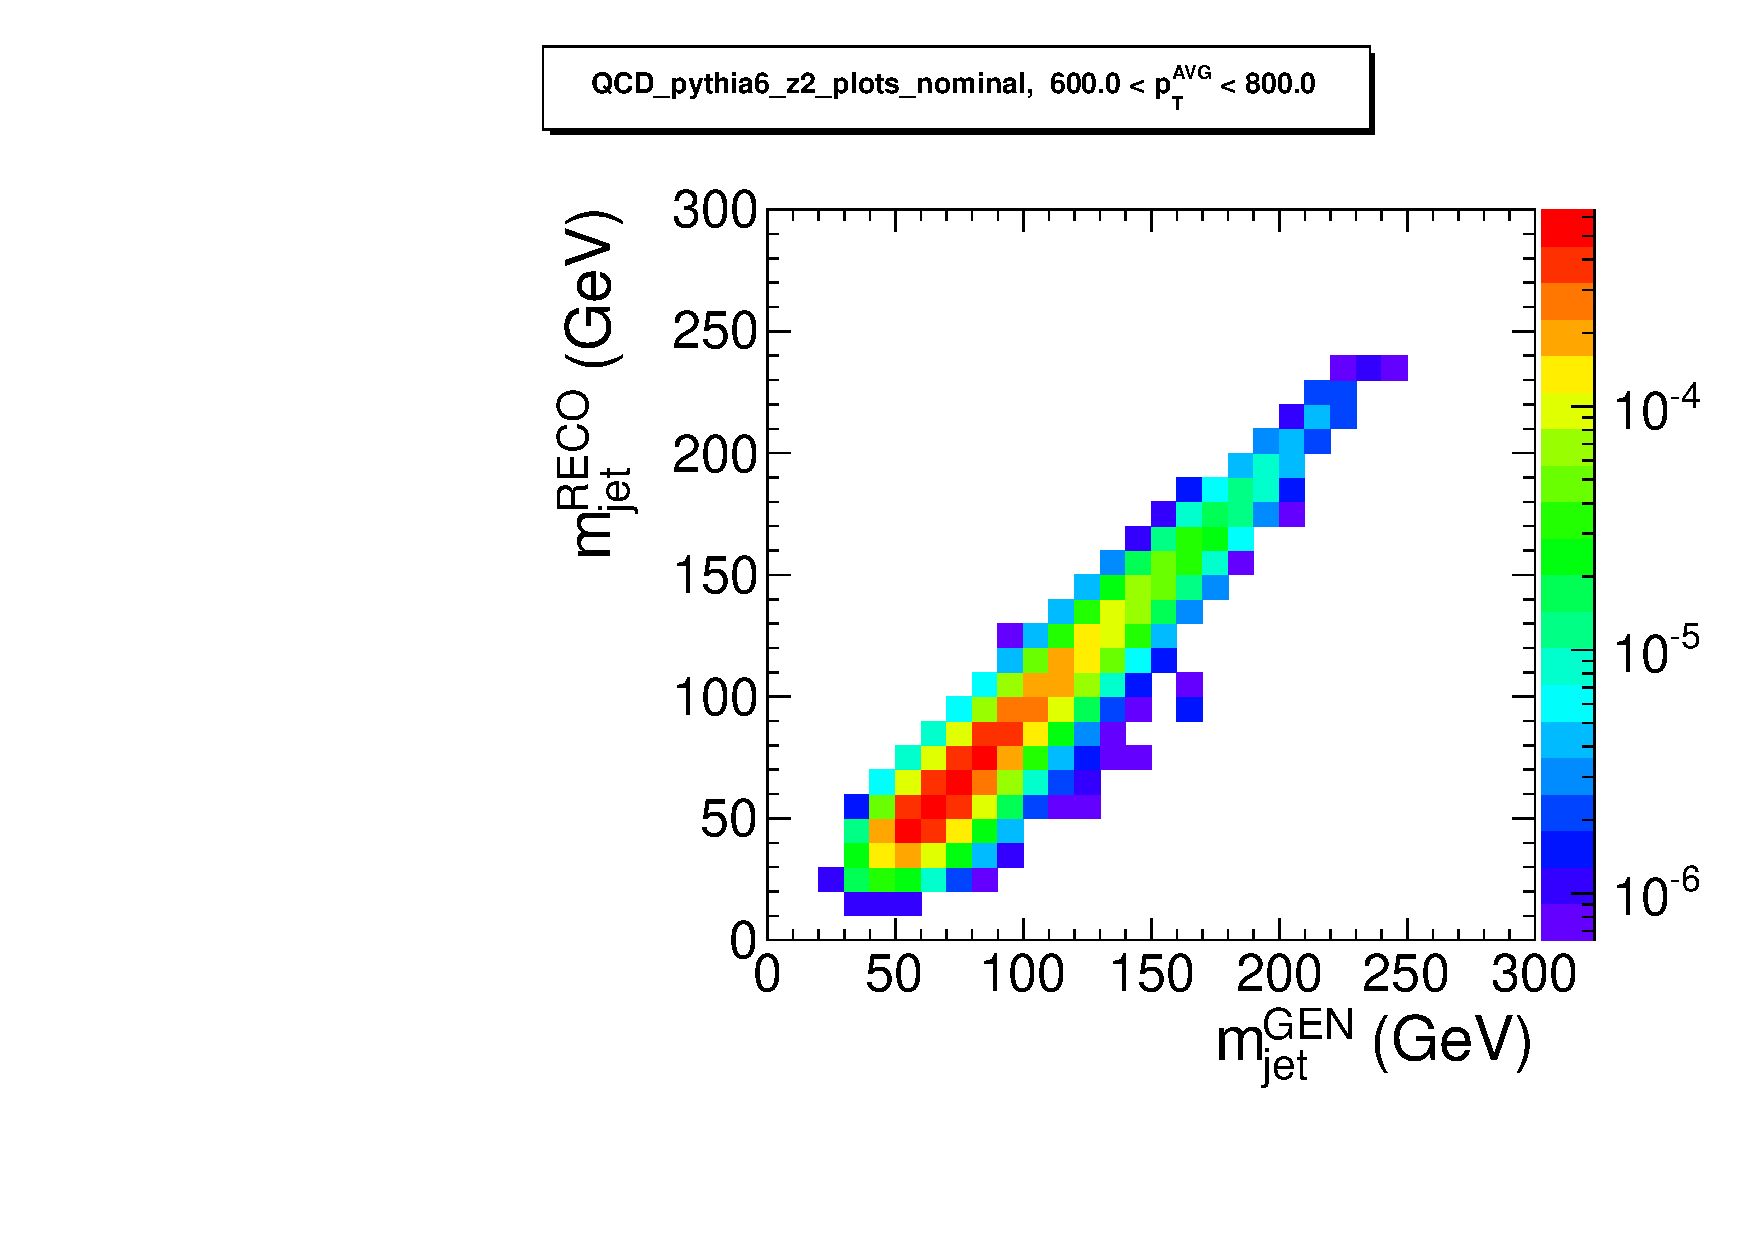
\includegraphics[width=0.3\textwidth]{figs/response_QCD_pythia6_z2_plots_nominal_pt8}}
\subfigure{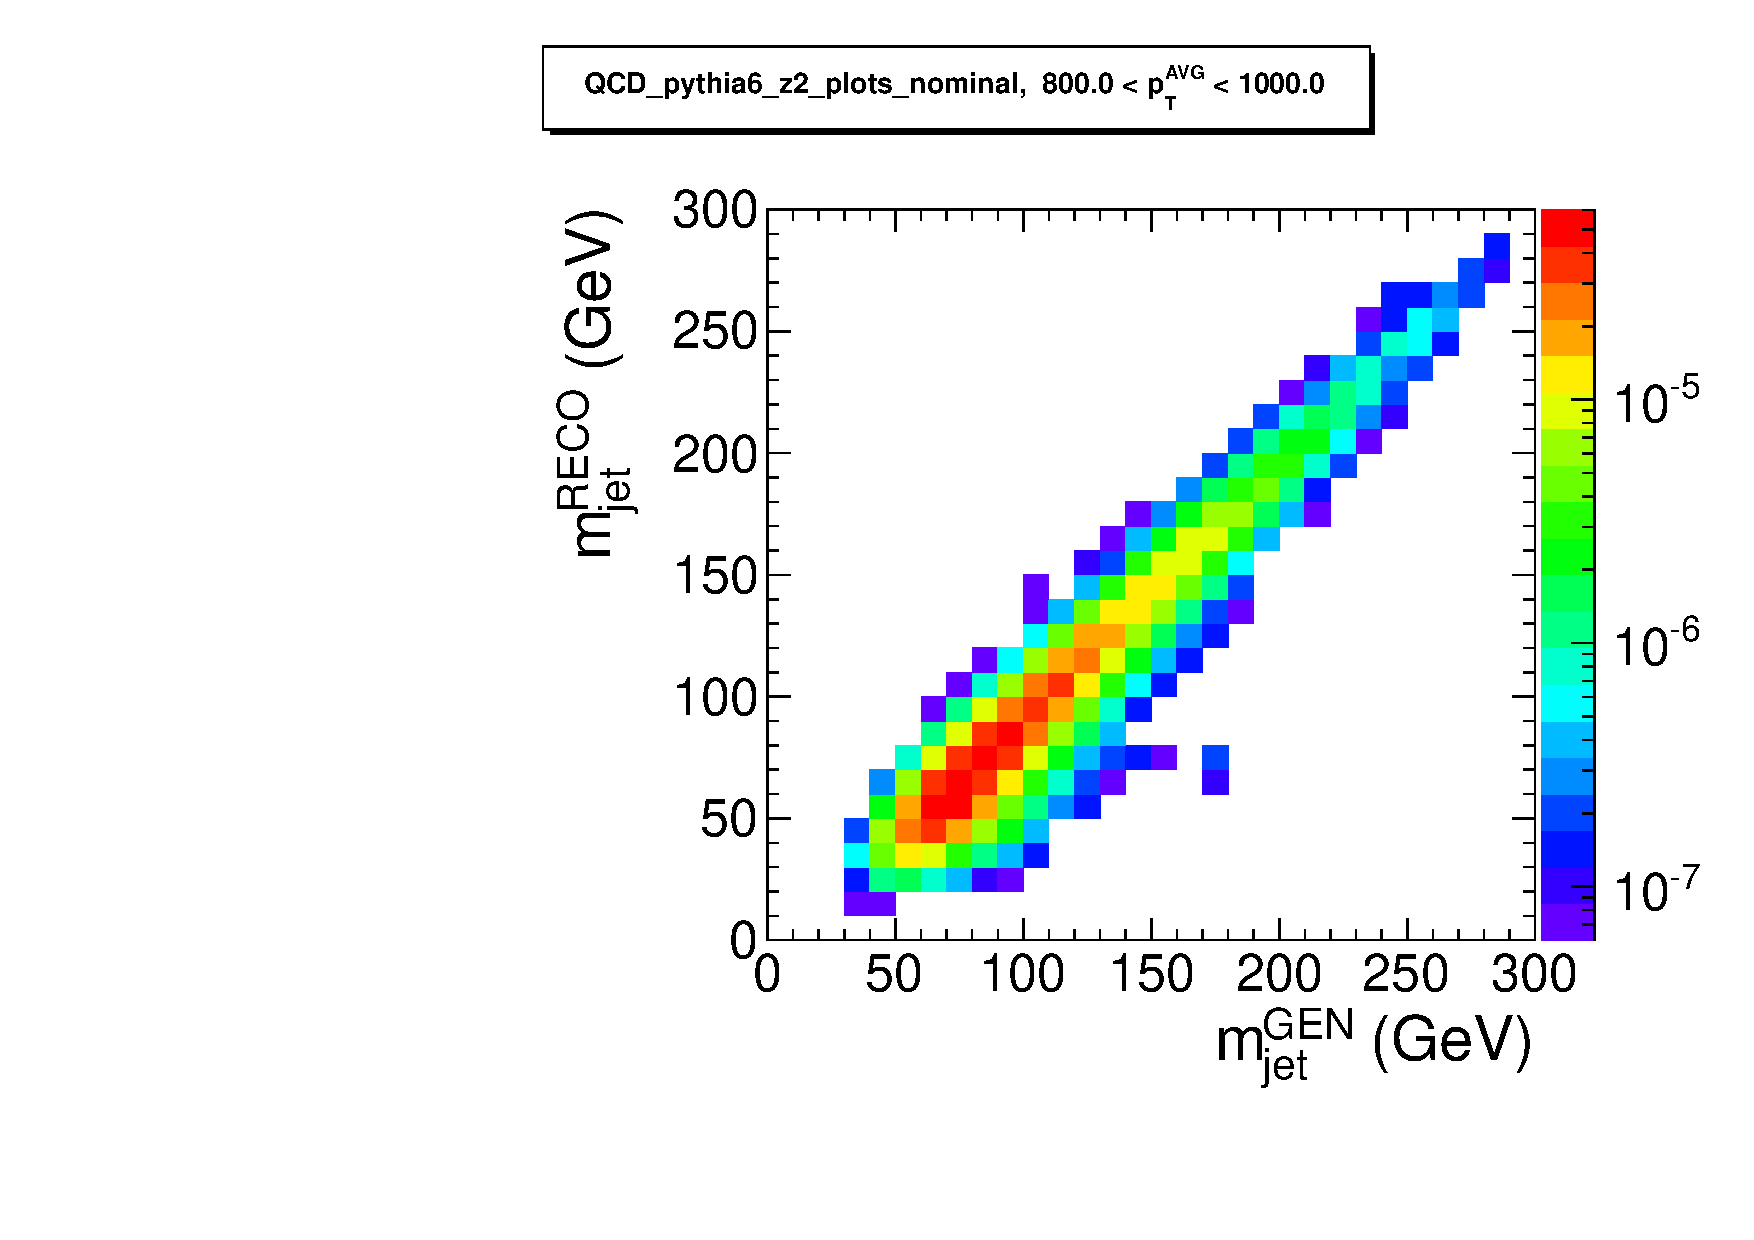
\includegraphics[width=0.3\textwidth]{figs/response_QCD_pythia6_z2_plots_nominal_pt9}}\\
\caption{Response of the jet mass for AK7 jets,
for various $\pt^{AVG}$ bins. The true jet mass is shown
on the $x-$axis, and the reconstructed jet mass is shown on the
$y-$axis, using the \PYTHIA generator. 
\label{figs:response_QCD_pythia6_z2_plots_nominal_ptall}}
\end{figure}


\clearpage

\begin{figure}[htbp]
\centering
\subfigure{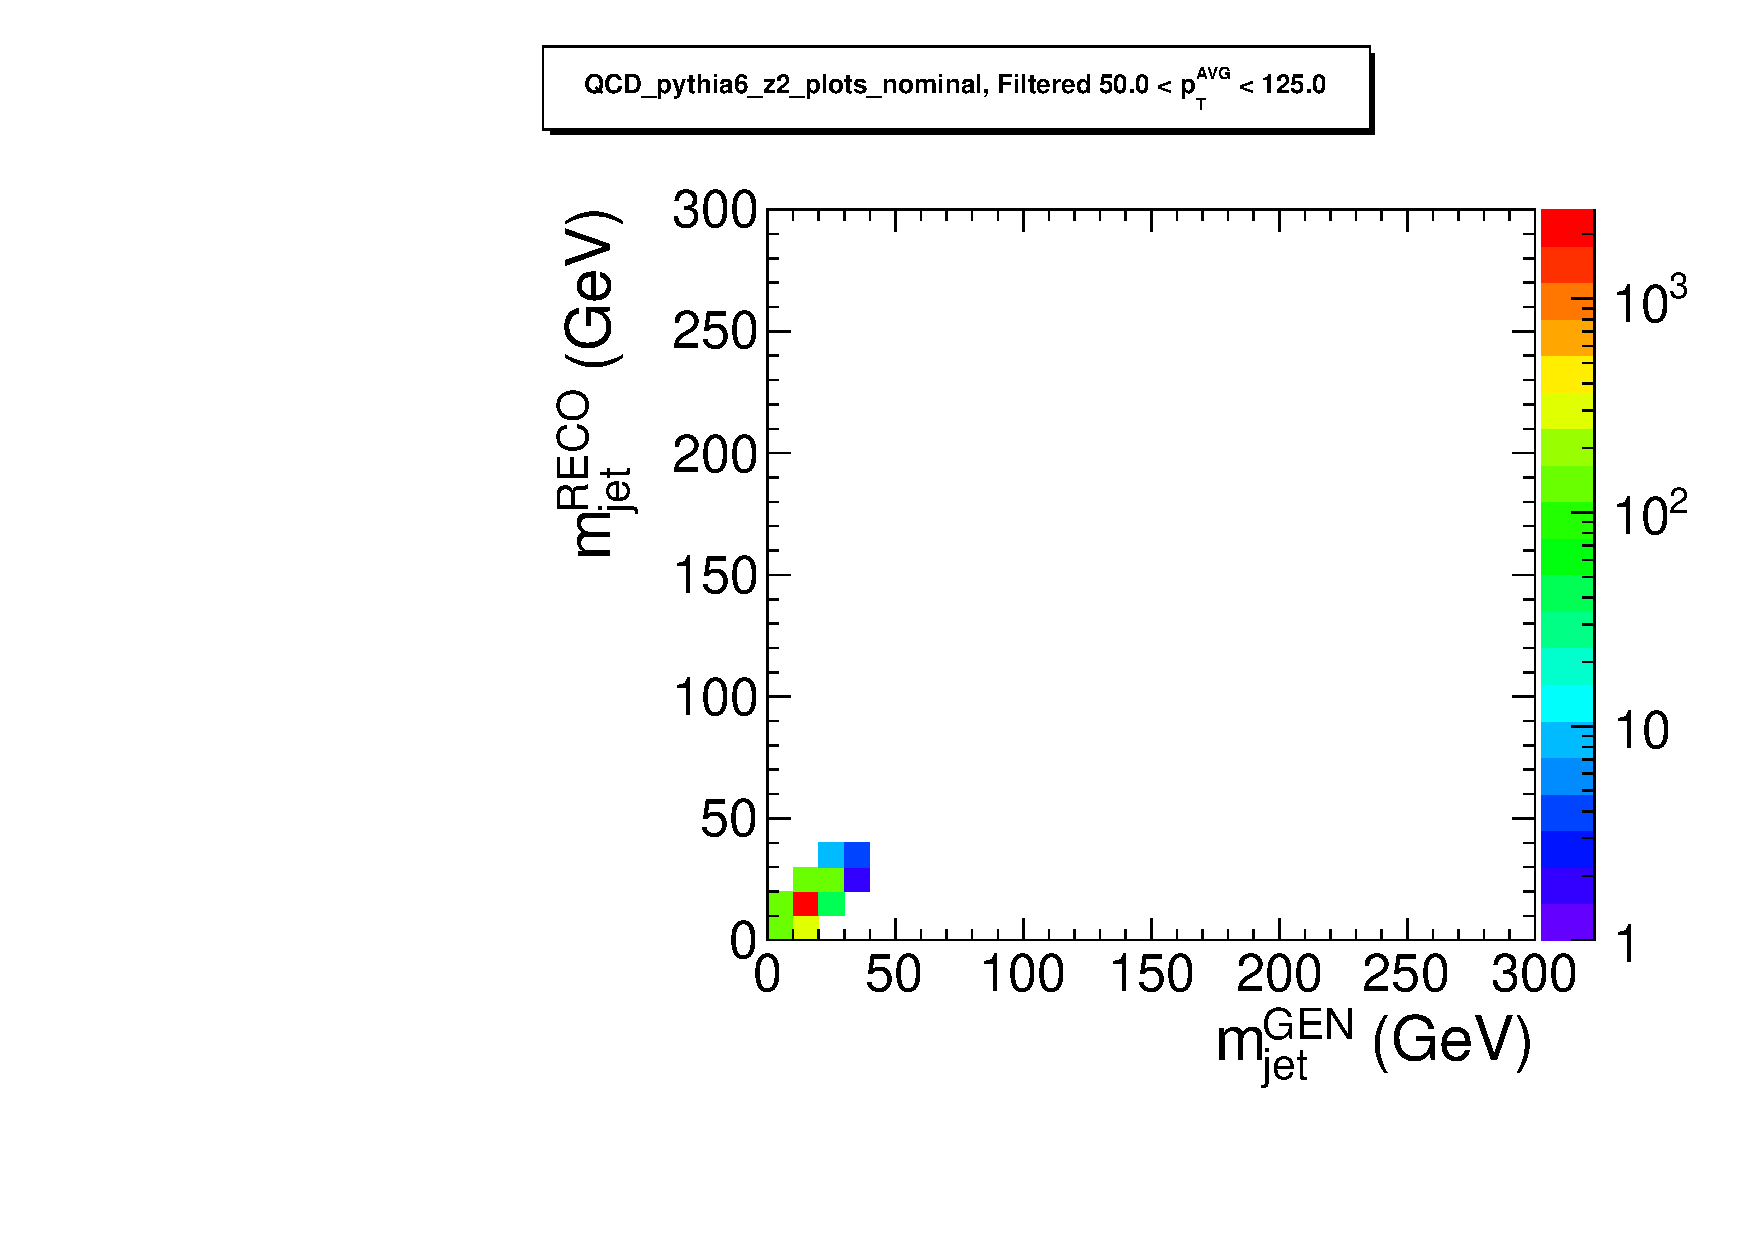
\includegraphics[width=0.3\textwidth]{figs/response_QCD_pythia6_z2_plots_nominal_Filtered_pt1}}
\subfigure{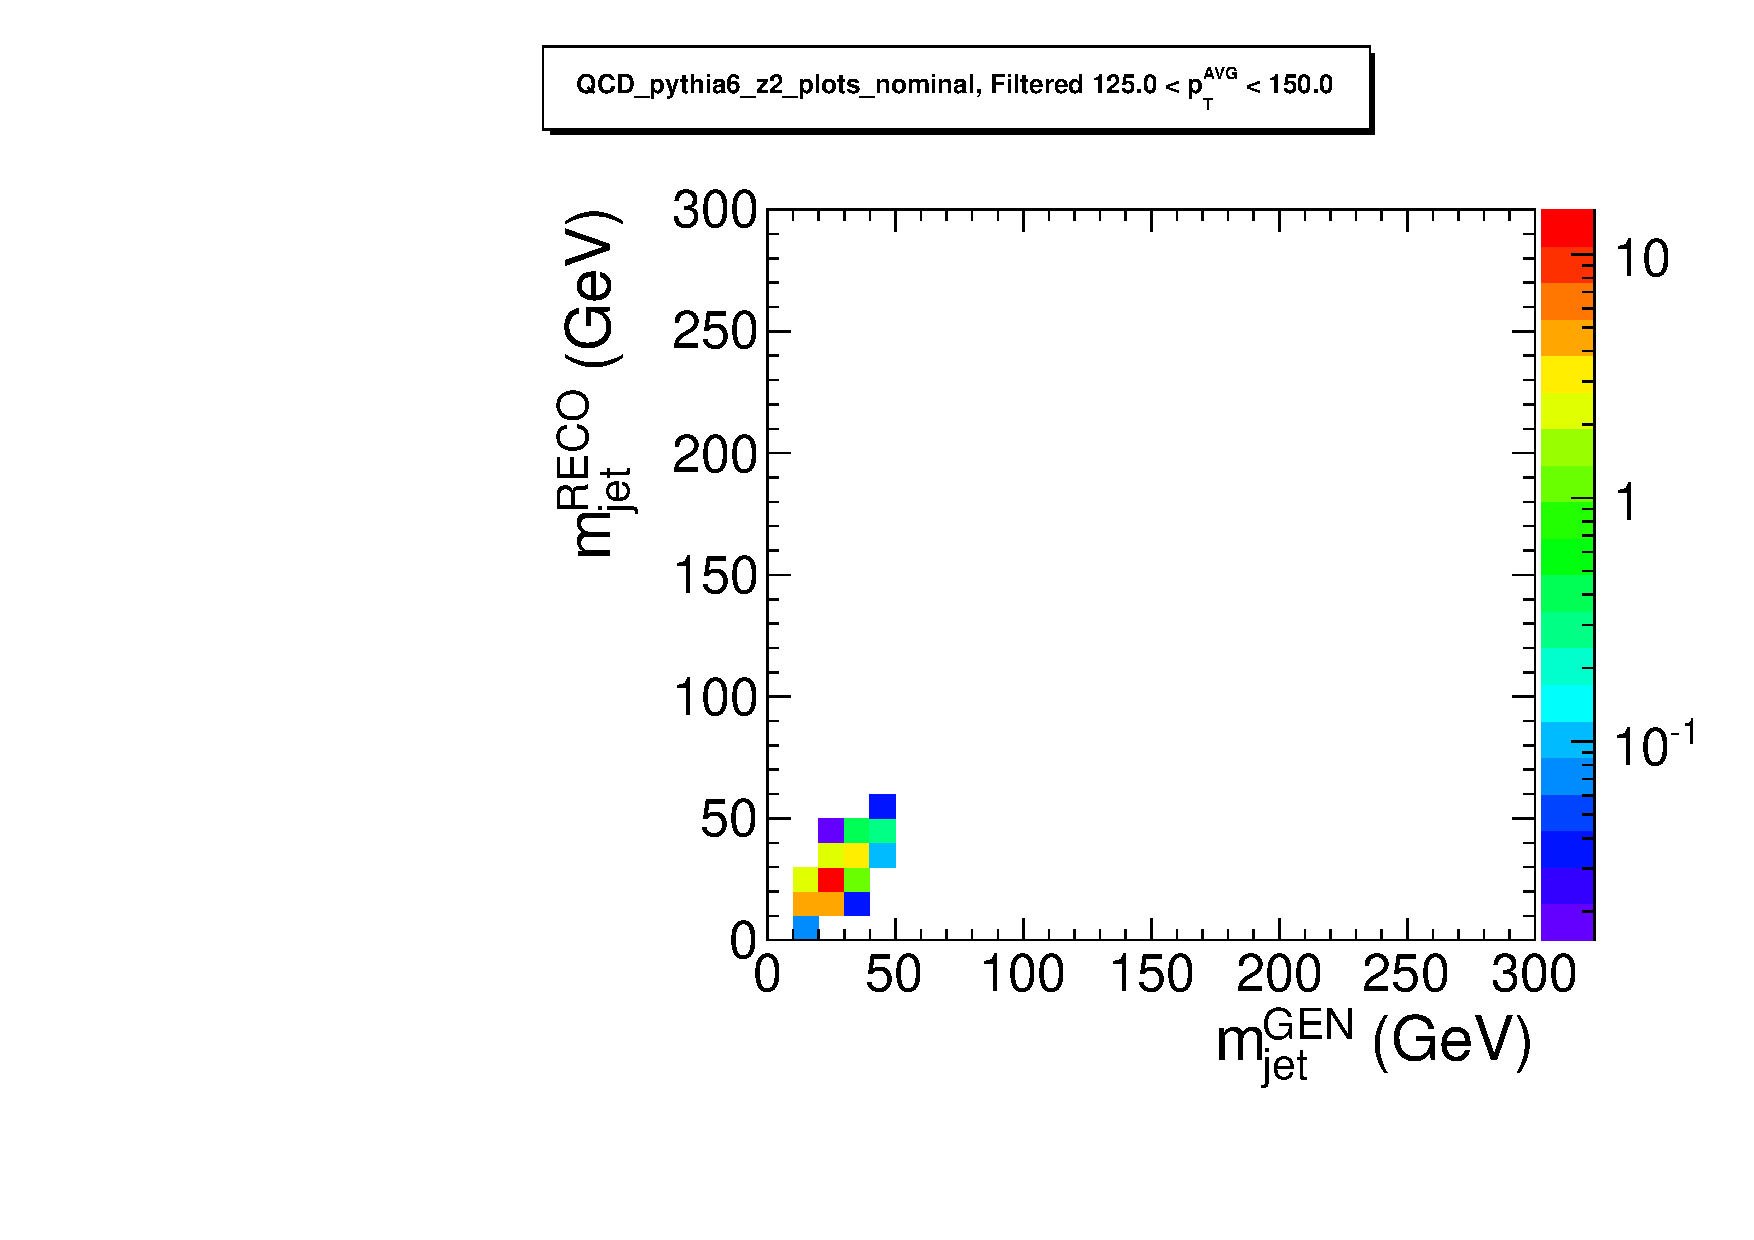
\includegraphics[width=0.3\textwidth]{figs/response_QCD_pythia6_z2_plots_nominal_Filtered_pt2}}
\subfigure{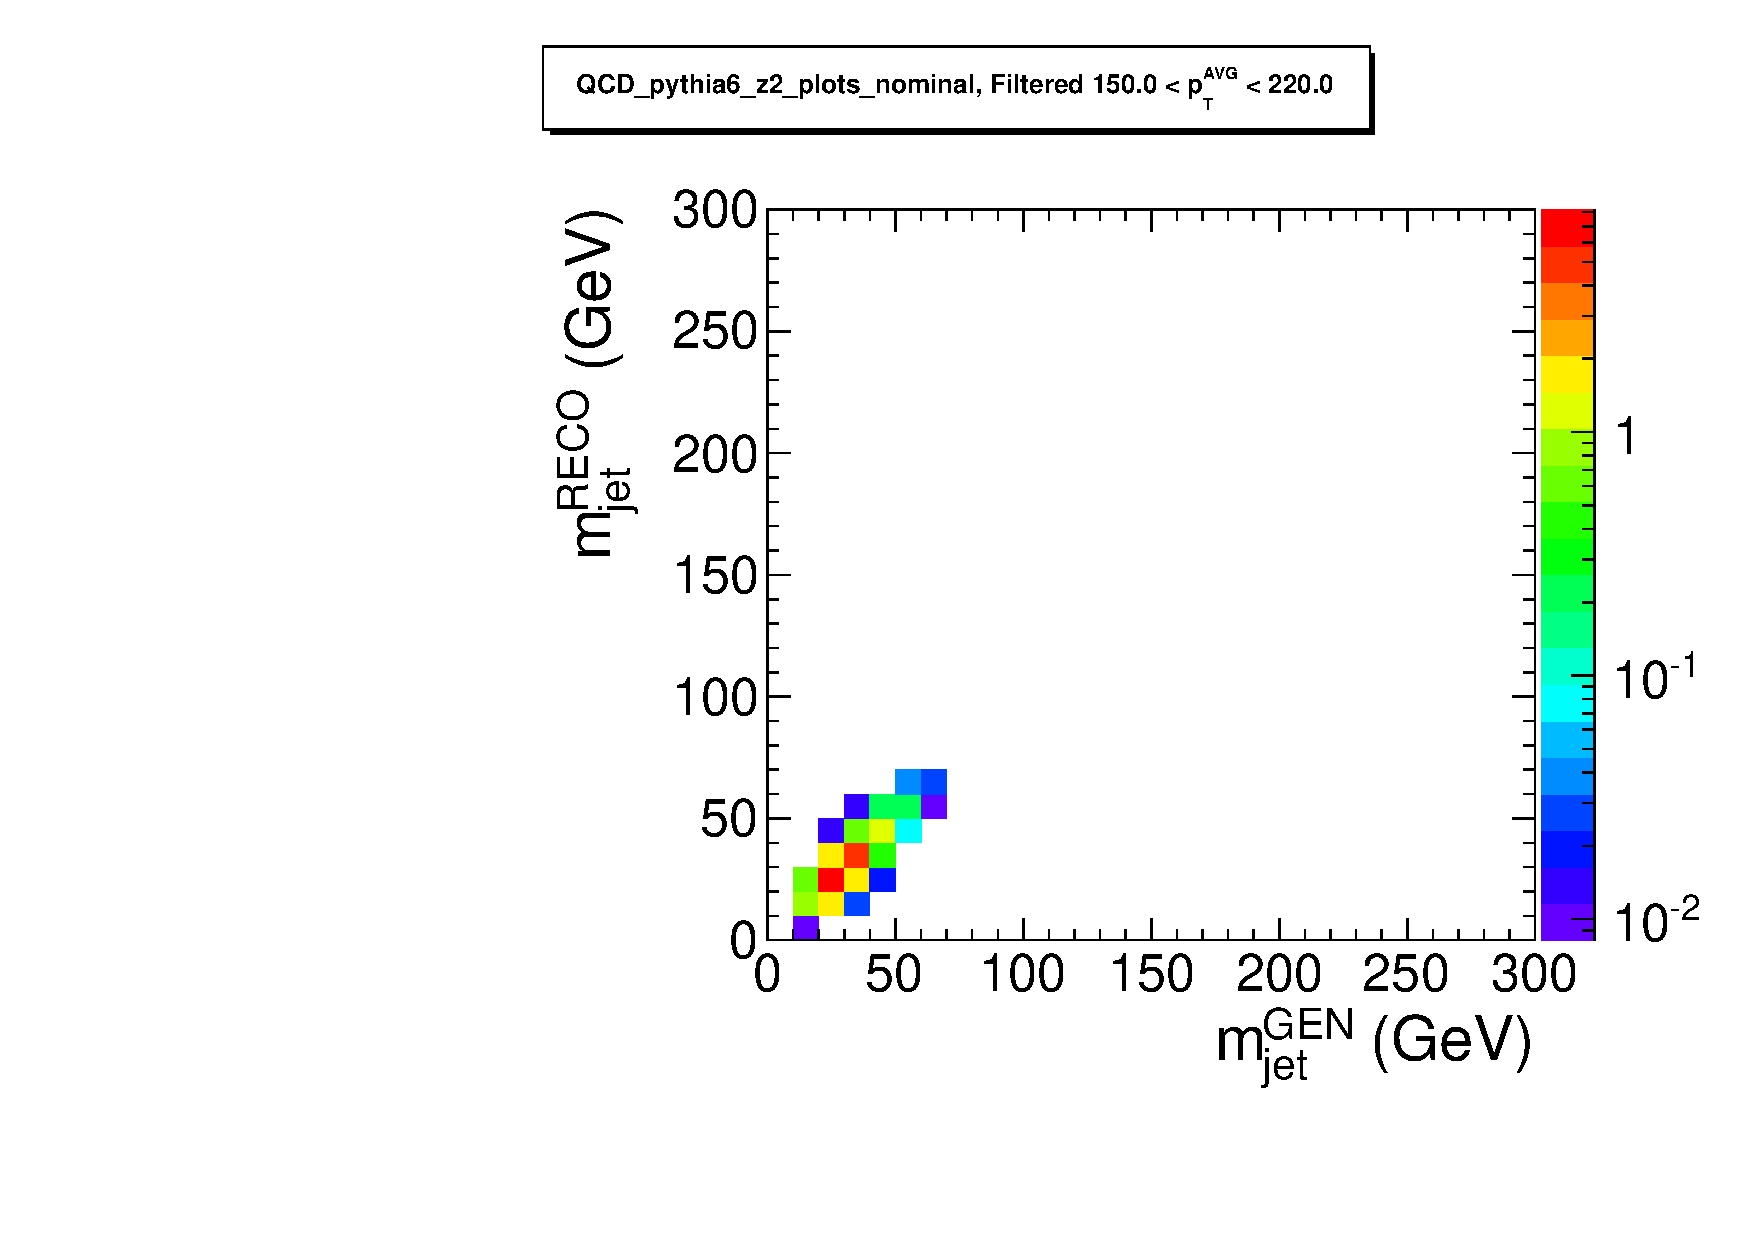
\includegraphics[width=0.3\textwidth]{figs/response_QCD_pythia6_z2_plots_nominal_Filtered_pt3}}\\
\subfigure{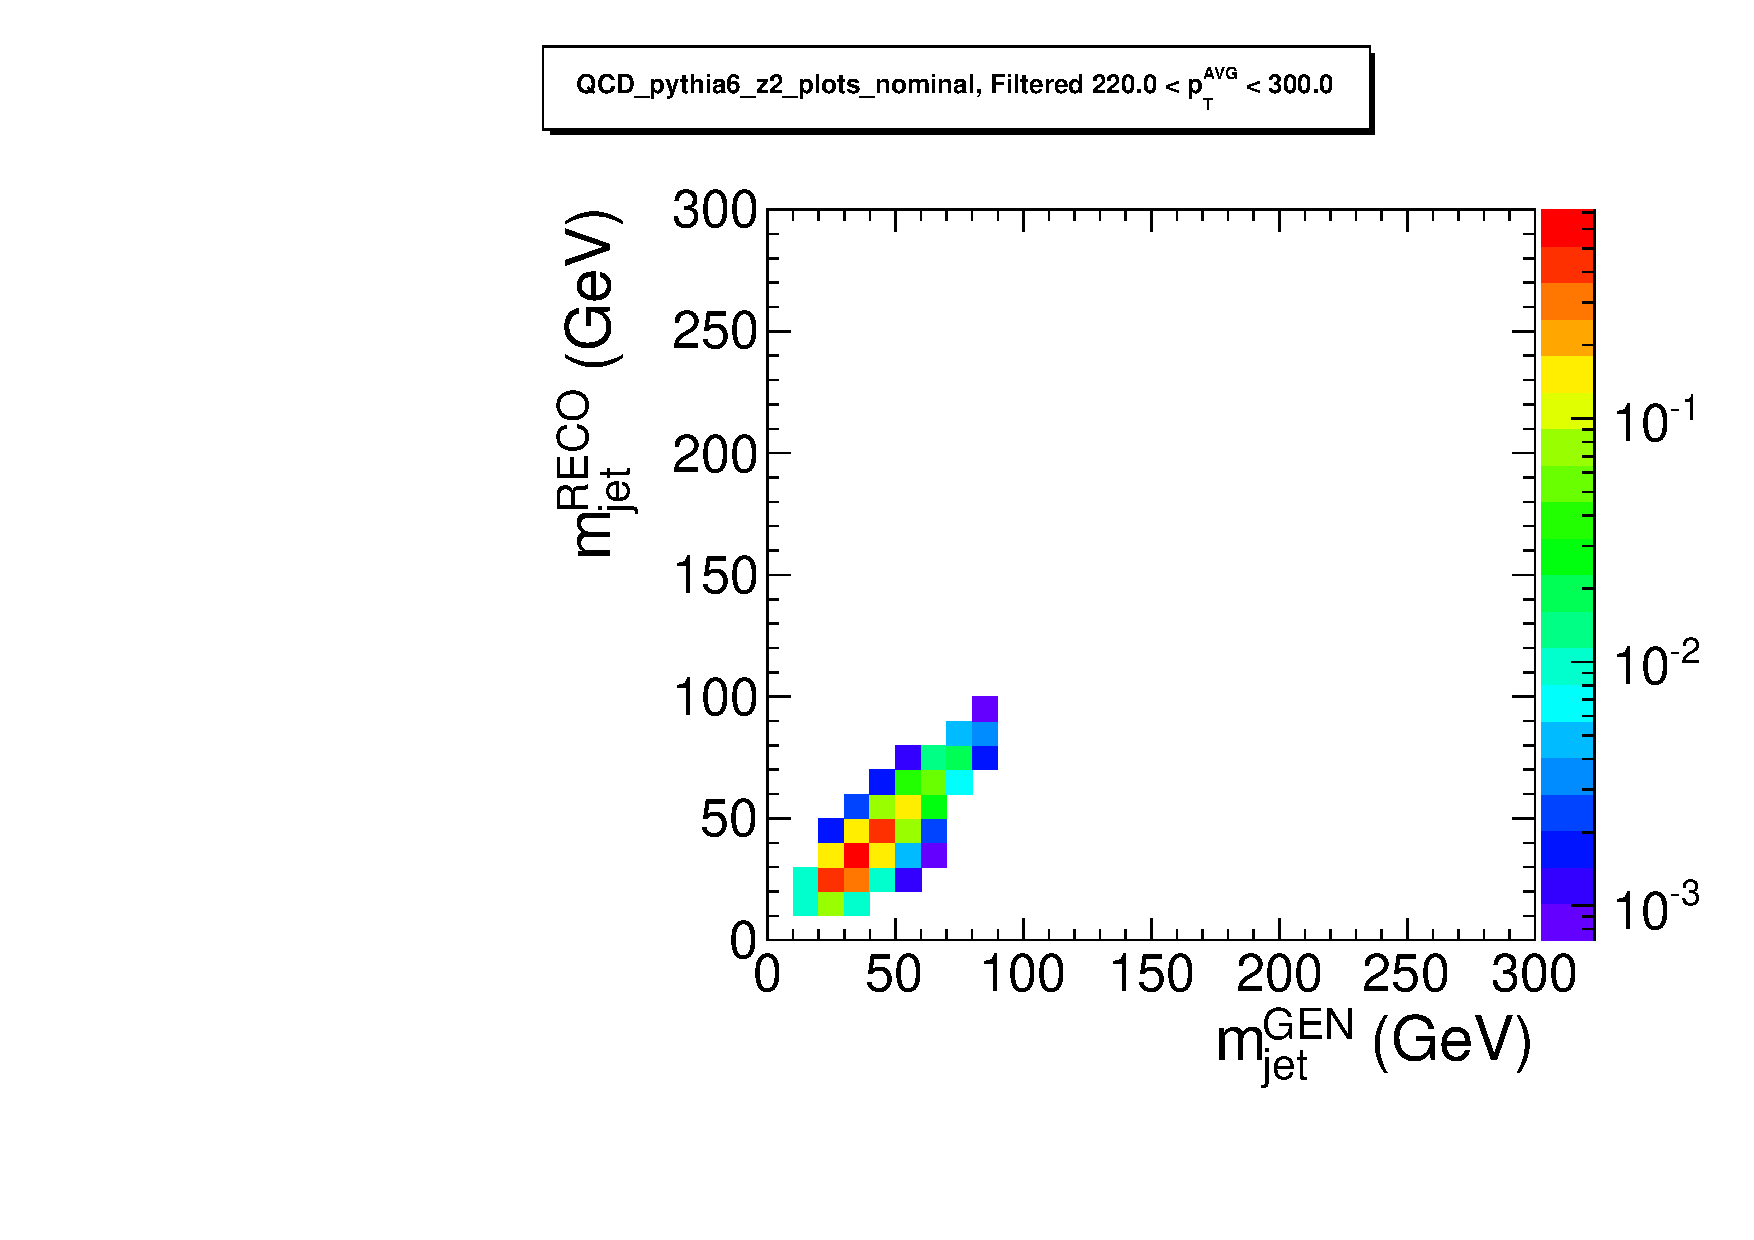
\includegraphics[width=0.3\textwidth]{figs/response_QCD_pythia6_z2_plots_nominal_Filtered_pt4}}
\subfigure{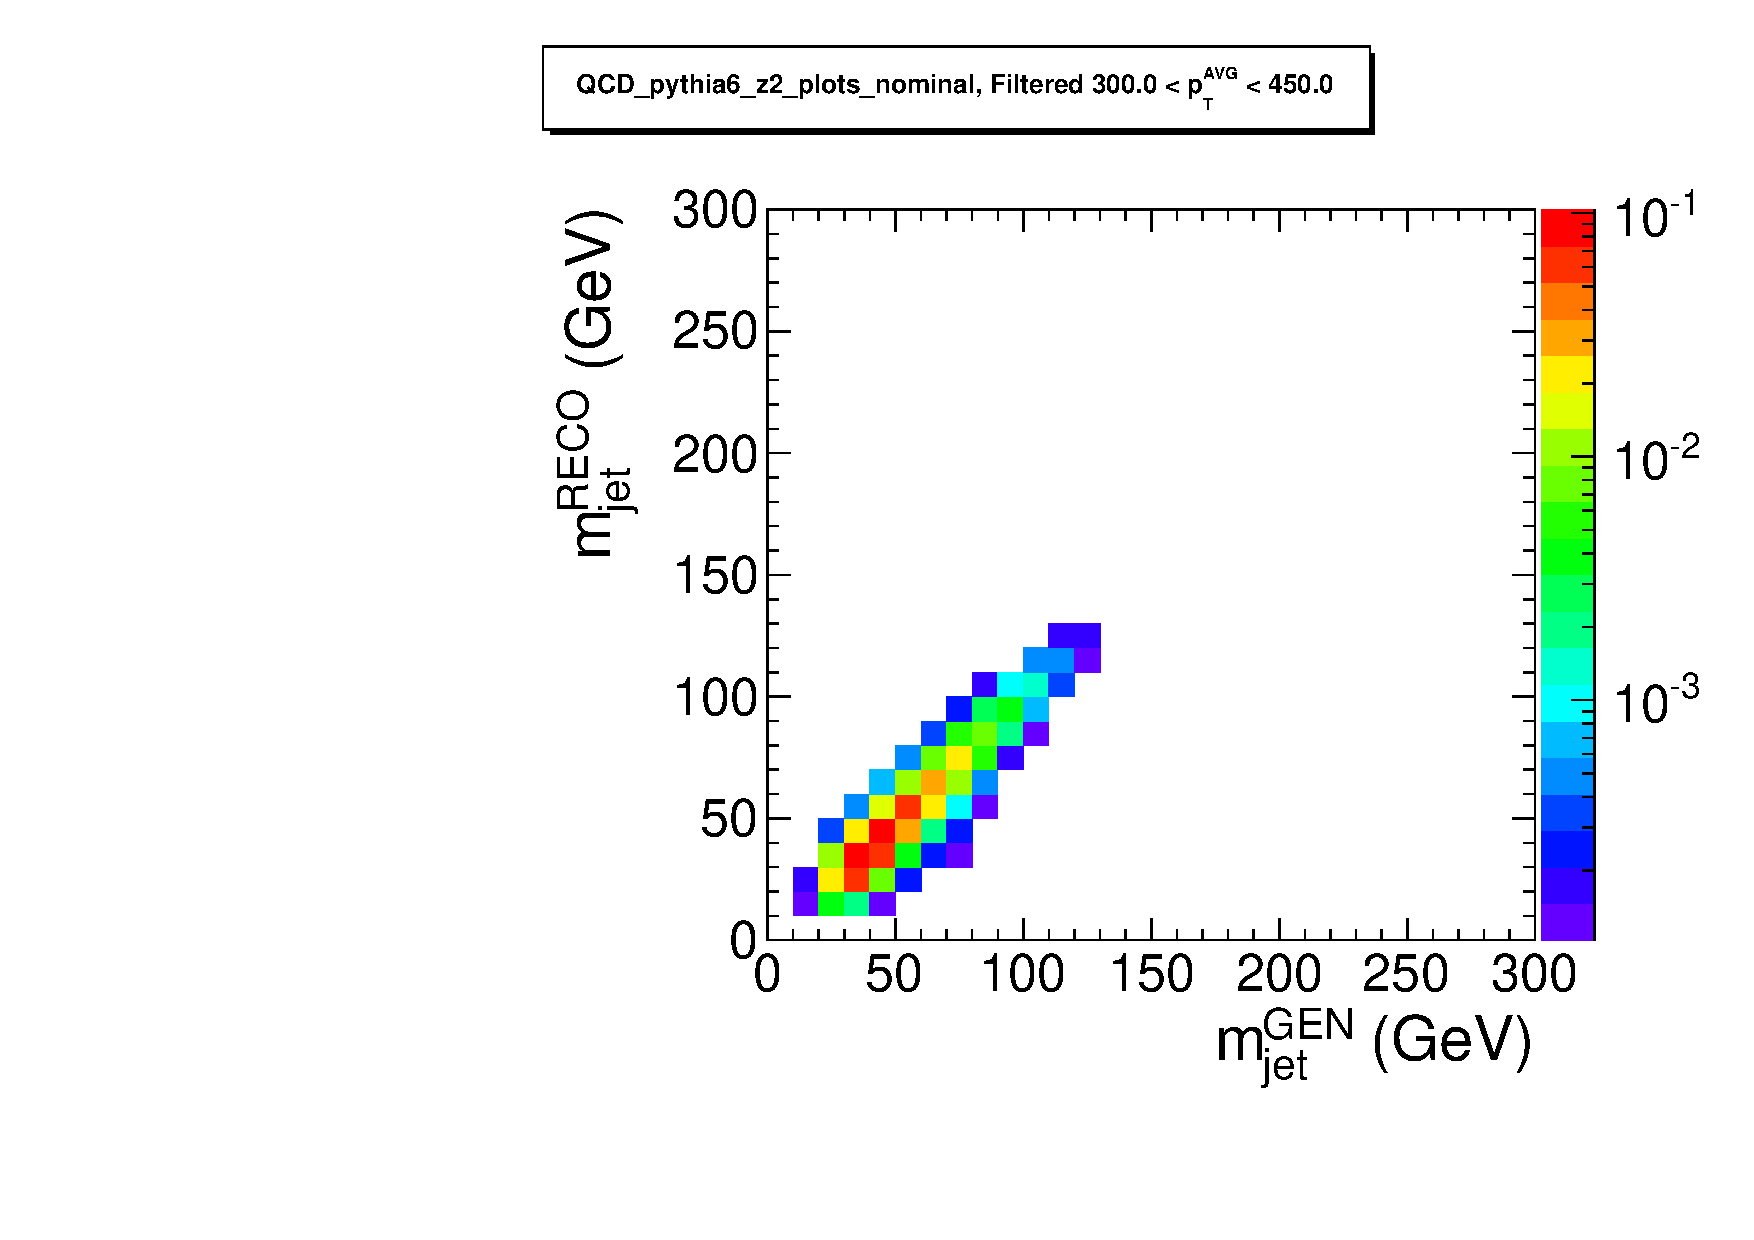
\includegraphics[width=0.3\textwidth]{figs/response_QCD_pythia6_z2_plots_nominal_Filtered_pt5}}
\subfigure{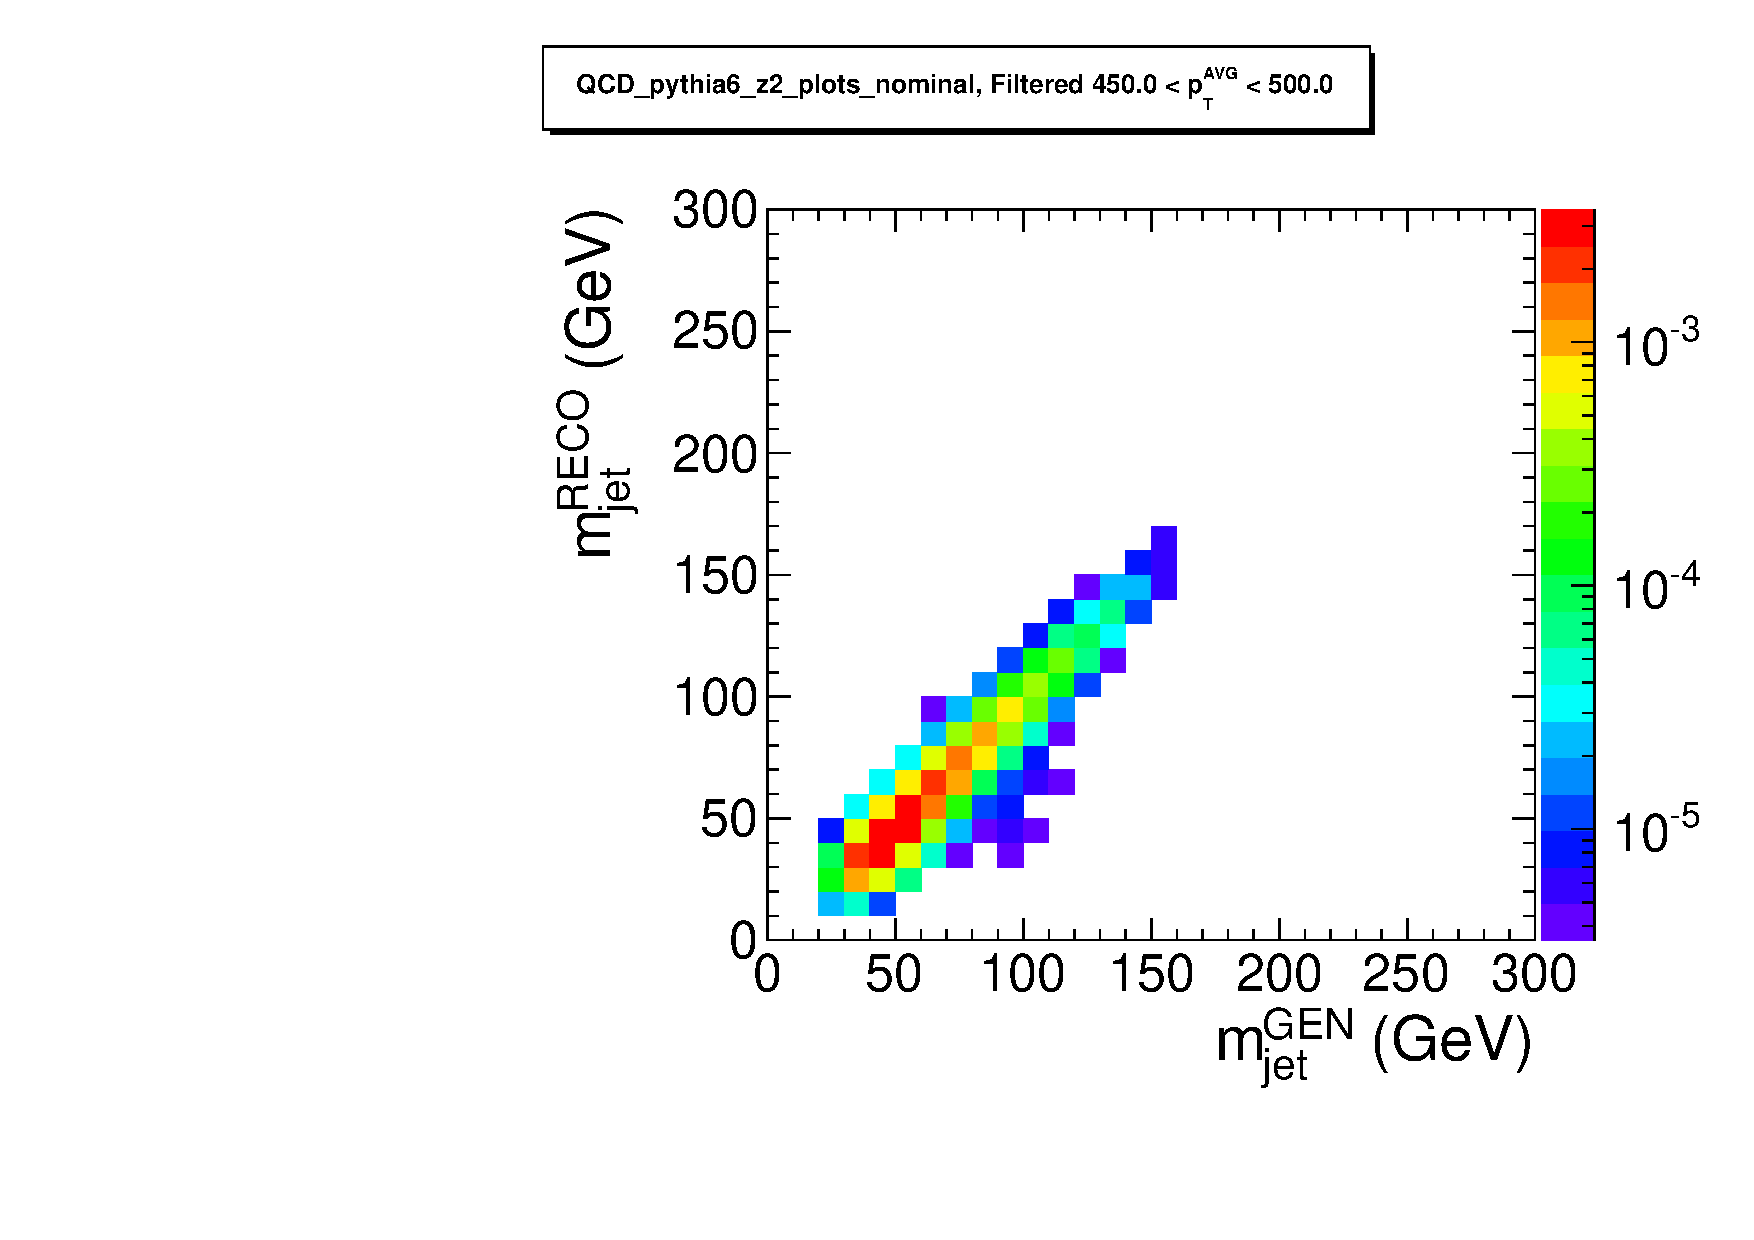
\includegraphics[width=0.3\textwidth]{figs/response_QCD_pythia6_z2_plots_nominal_Filtered_pt6}}\\
\subfigure{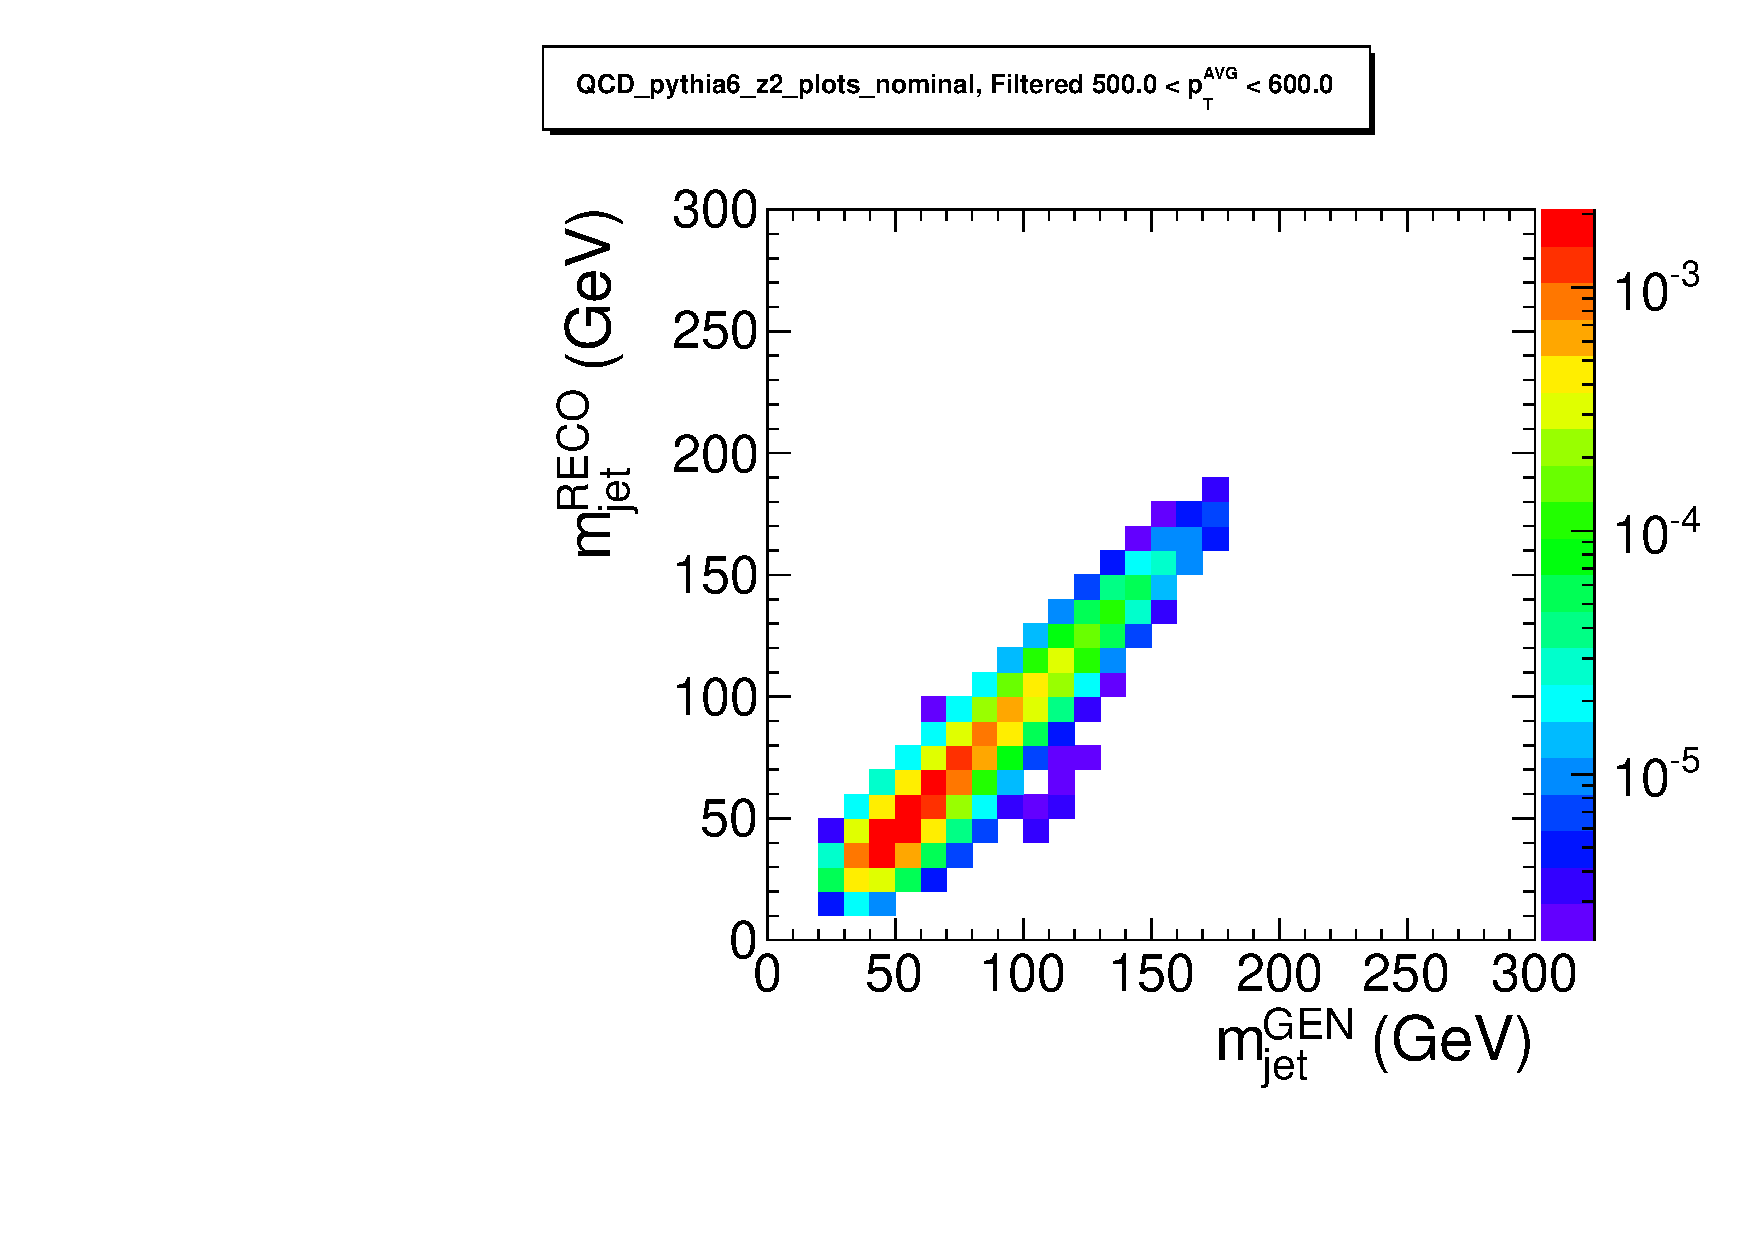
\includegraphics[width=0.3\textwidth]{figs/response_QCD_pythia6_z2_plots_nominal_Filtered_pt7}}
\subfigure{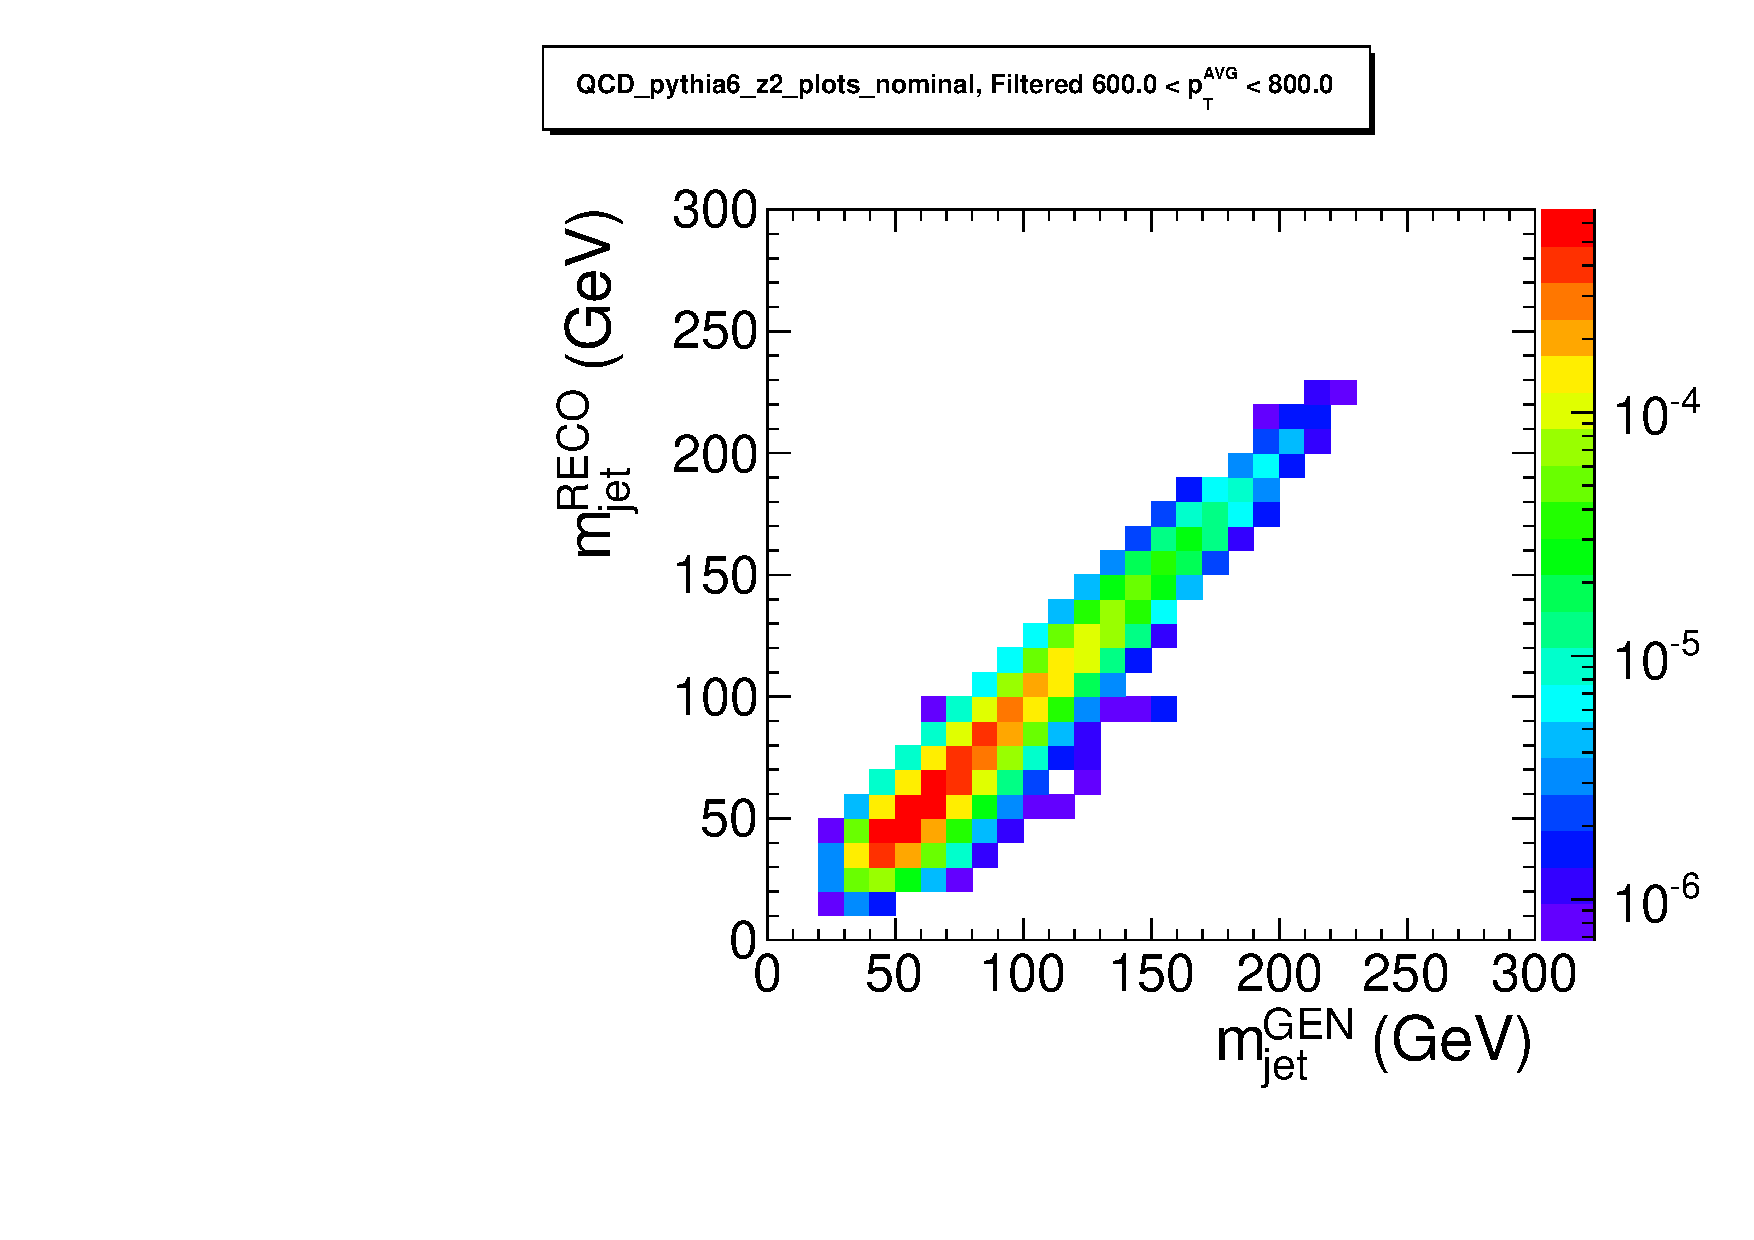
\includegraphics[width=0.3\textwidth]{figs/response_QCD_pythia6_z2_plots_nominal_Filtered_pt8}}
\subfigure{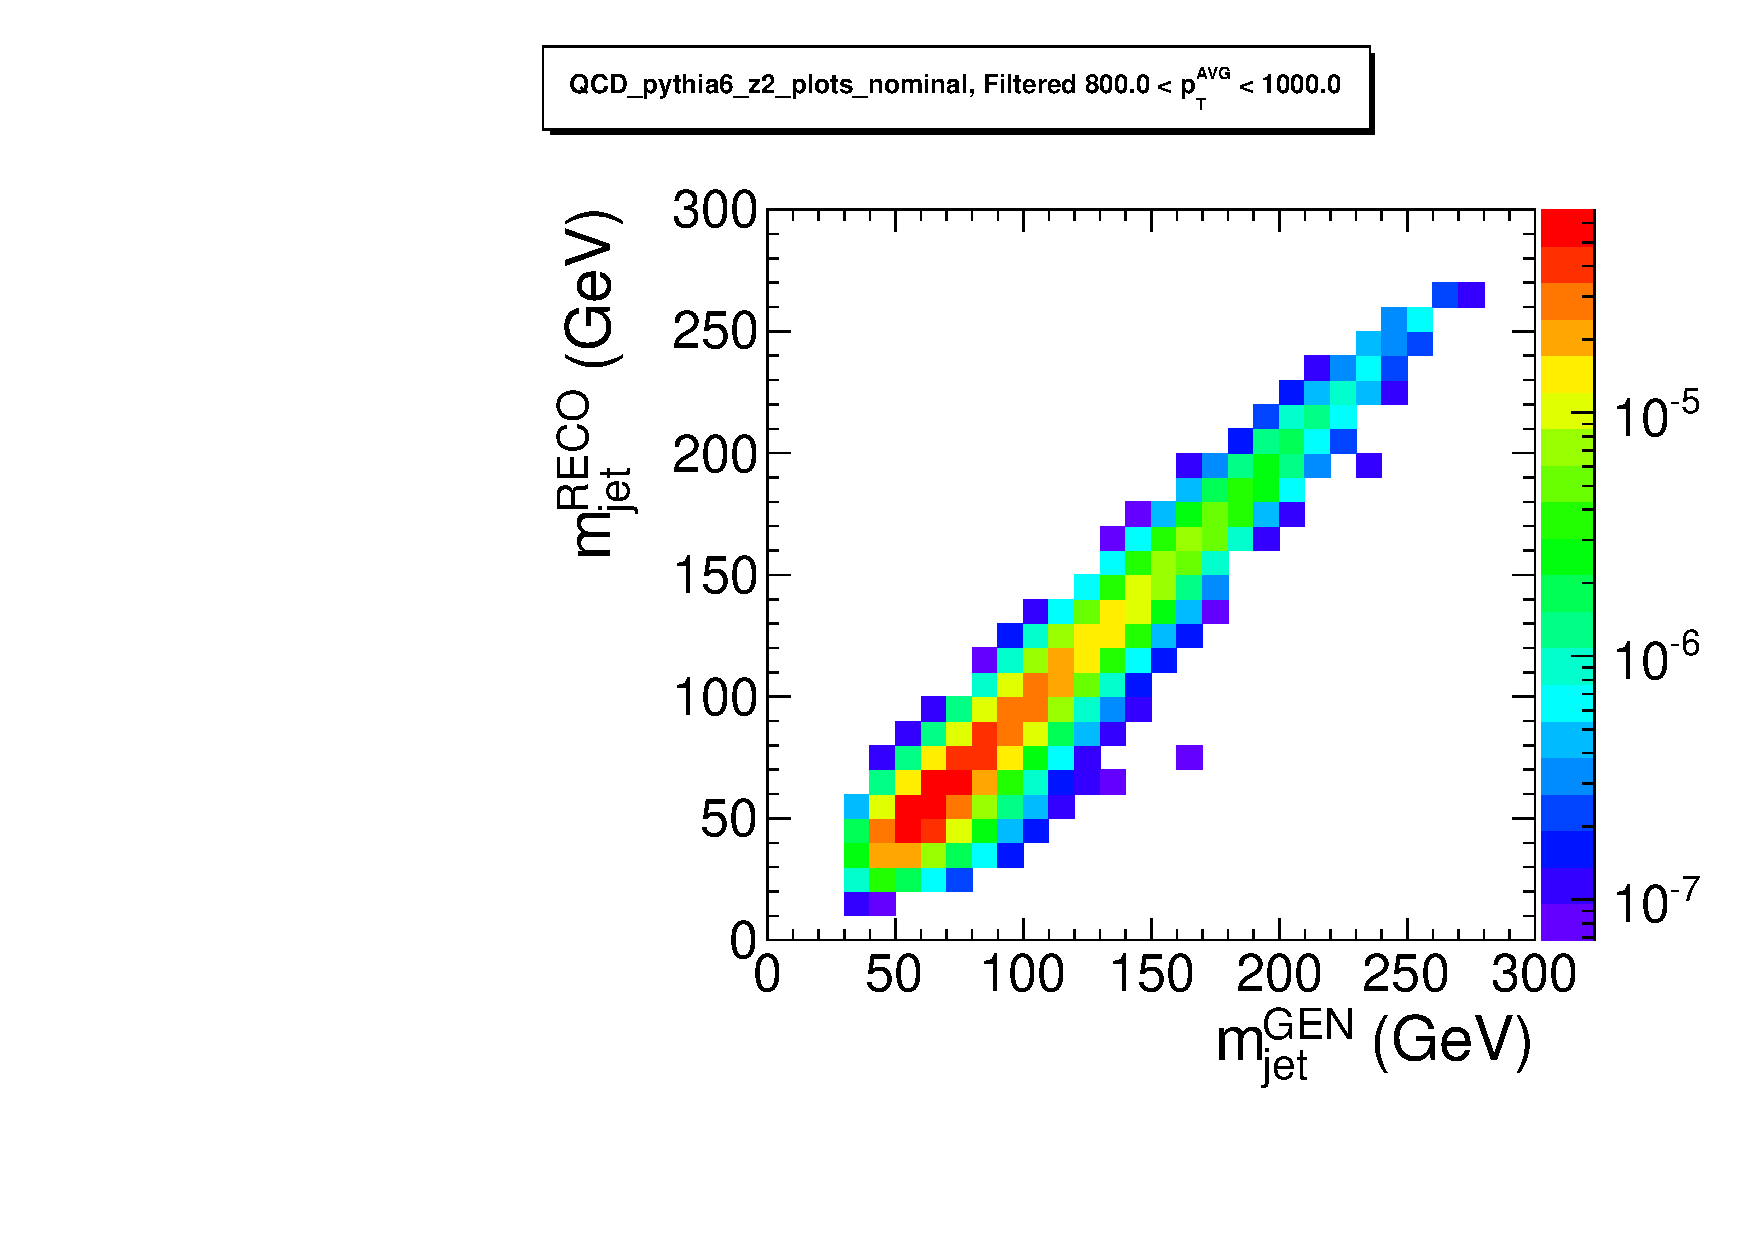
\includegraphics[width=0.3\textwidth]{figs/response_QCD_pythia6_z2_plots_nominal_Filtered_pt9}}\\
\caption{Response of the jet mass for AK7 Filteredjets,
for various $\pt^{AVG}$ bins. The true jet mass is shown
on the $x-$axis, and the reconstructed jet mass is shown on the
$y-$axis, using the \PYTHIA generator. 
\label{figs:response_QCD_pythia6_z2_plots_nominal_Filtered_ptall}}
\end{figure}


\clearpage

\begin{figure}[htbp]
\centering
\subfigure{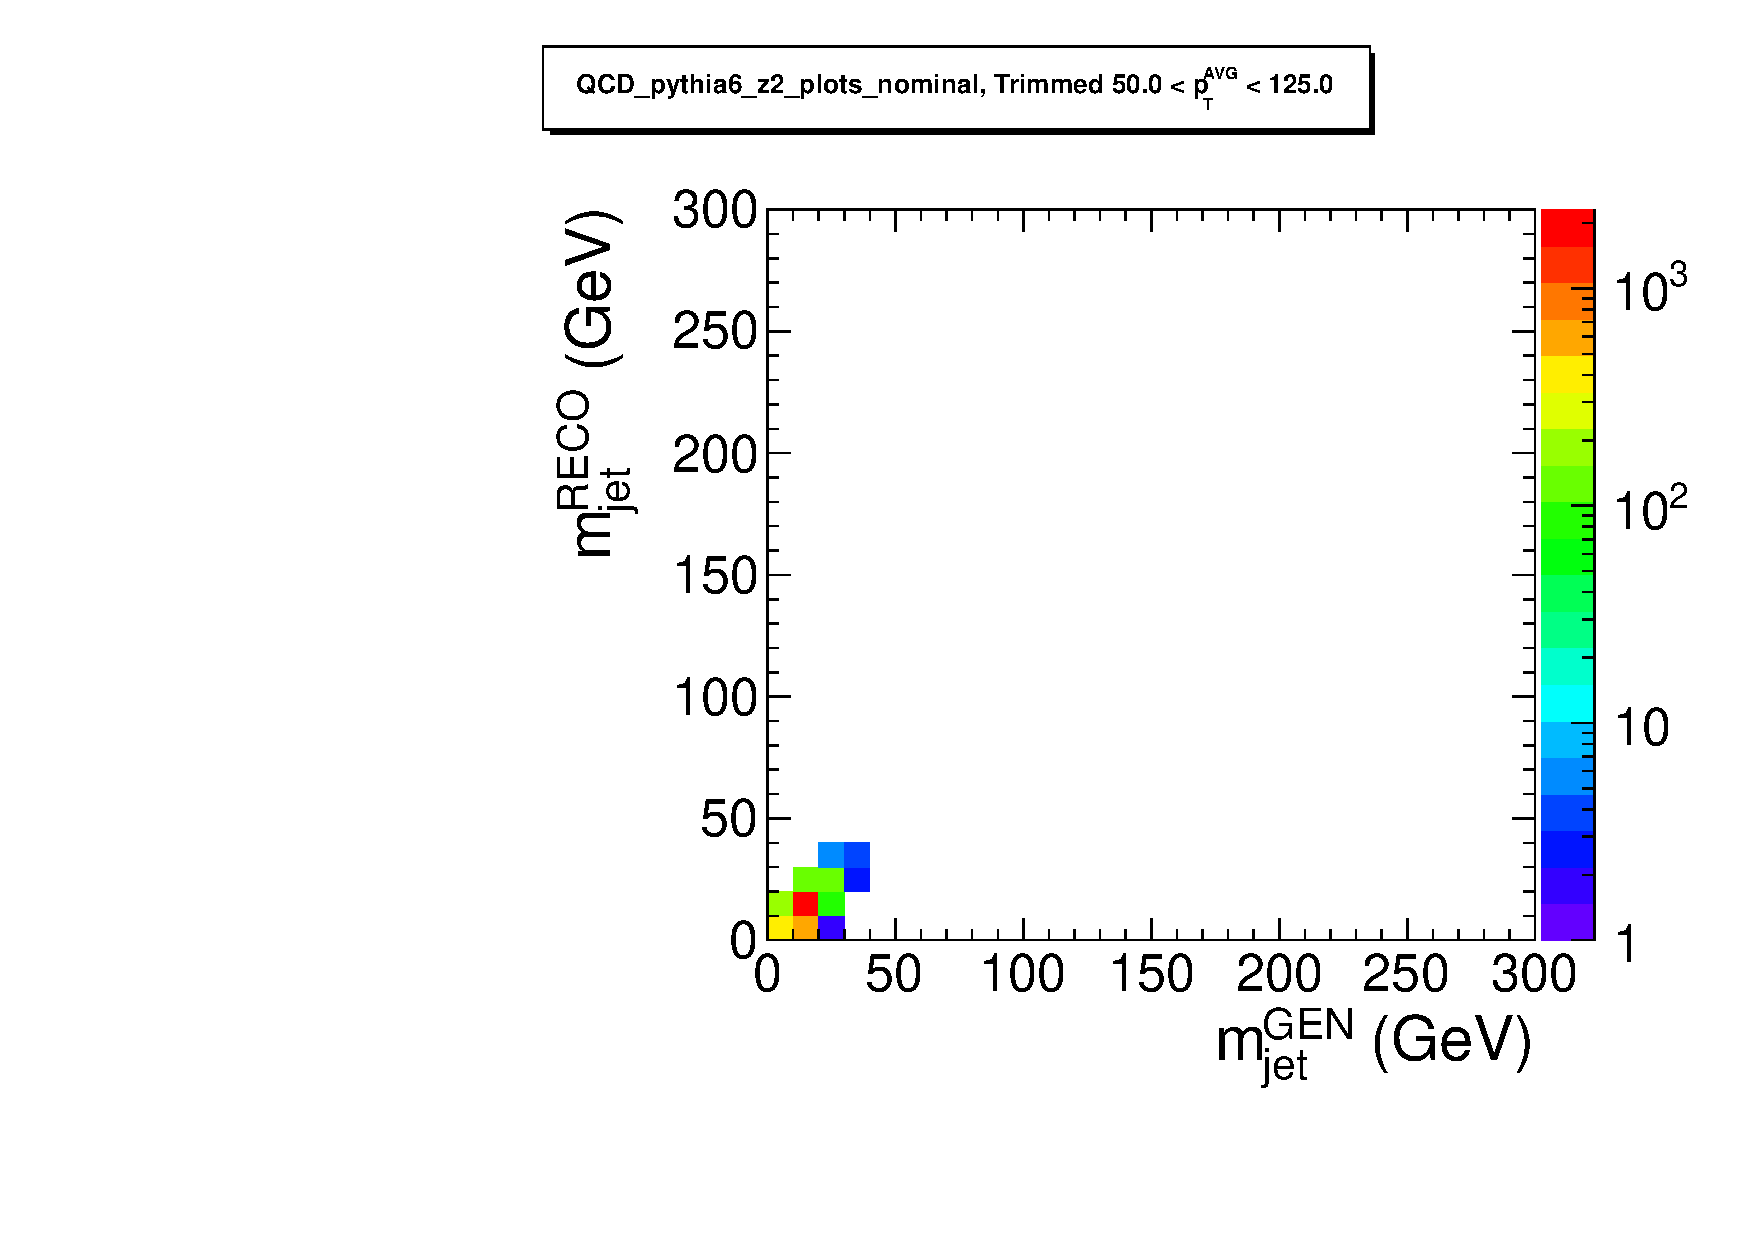
\includegraphics[width=0.3\textwidth]{figs/response_QCD_pythia6_z2_plots_nominal_Trimmed_pt1}}
\subfigure{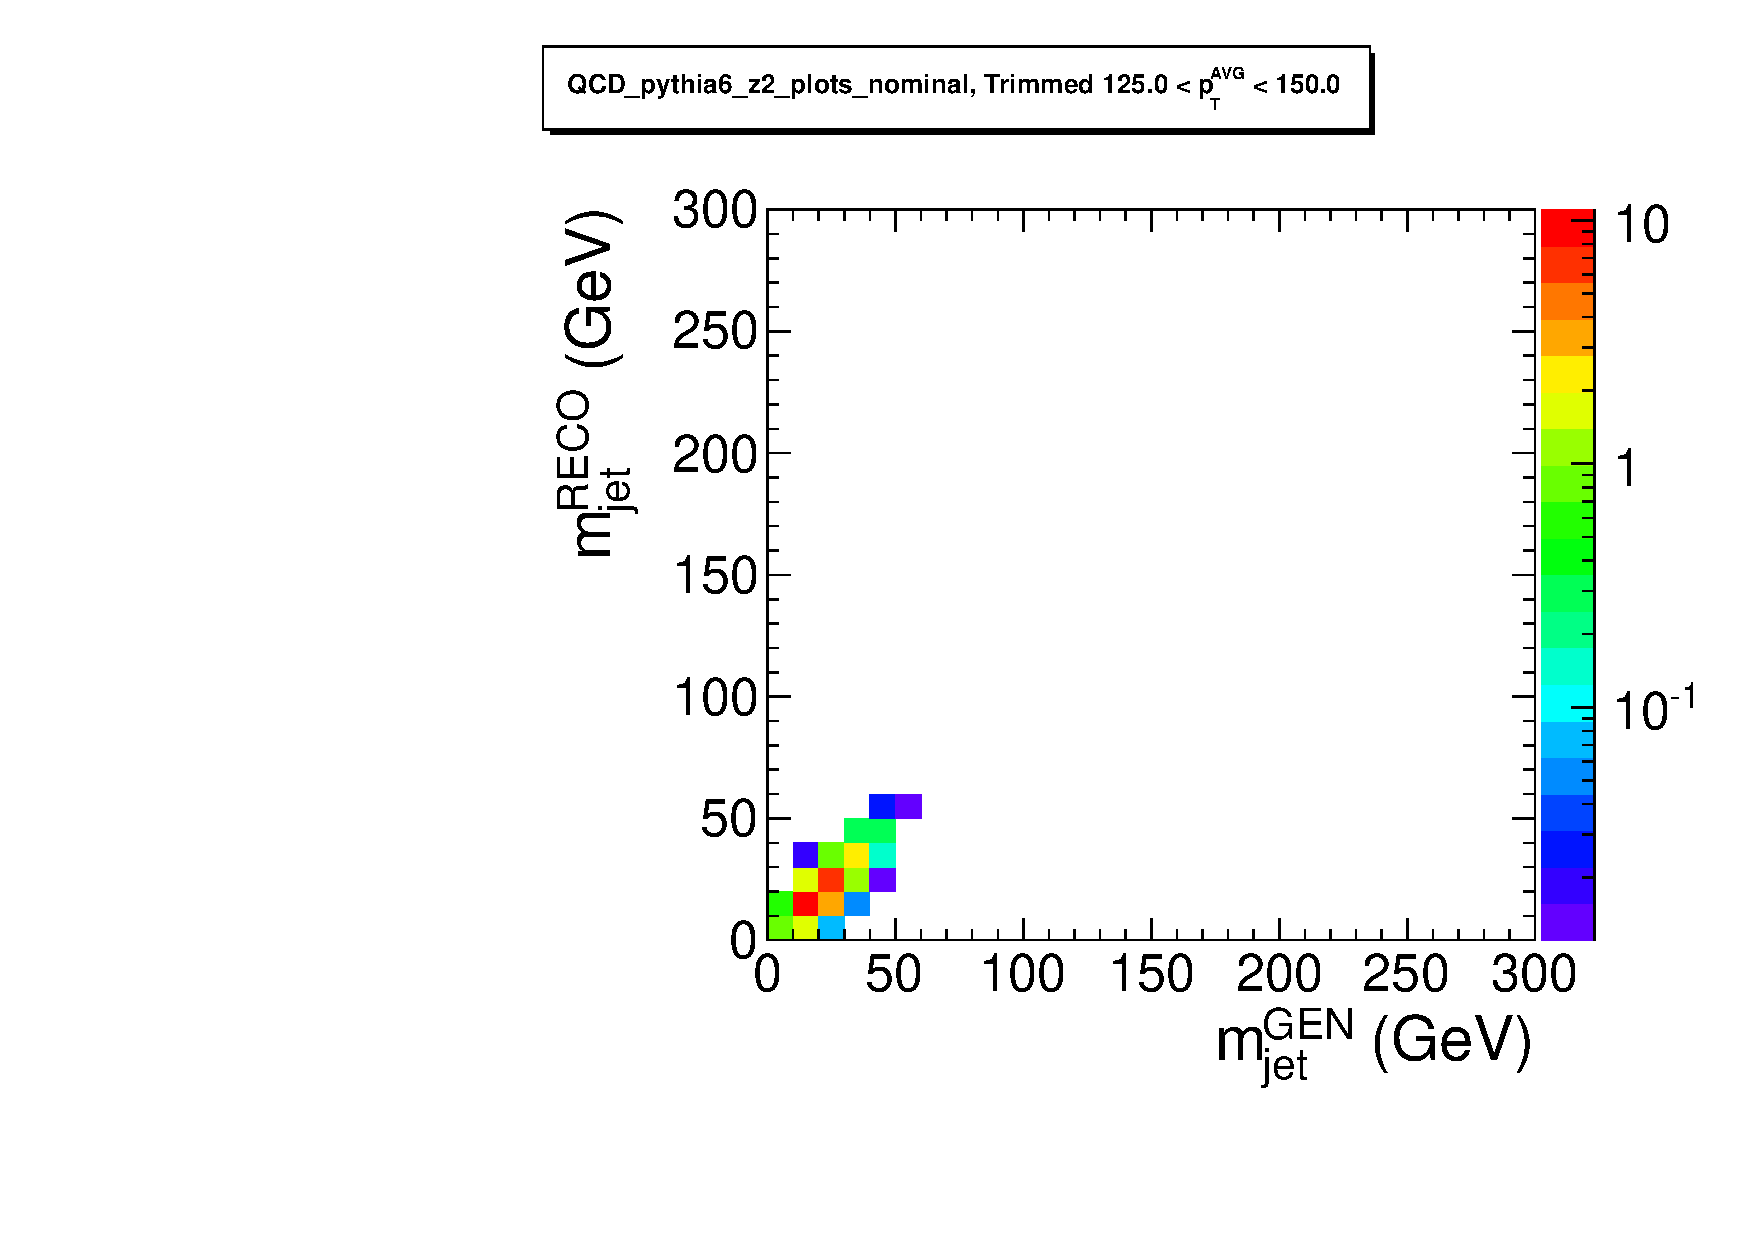
\includegraphics[width=0.3\textwidth]{figs/response_QCD_pythia6_z2_plots_nominal_Trimmed_pt2}}
\subfigure{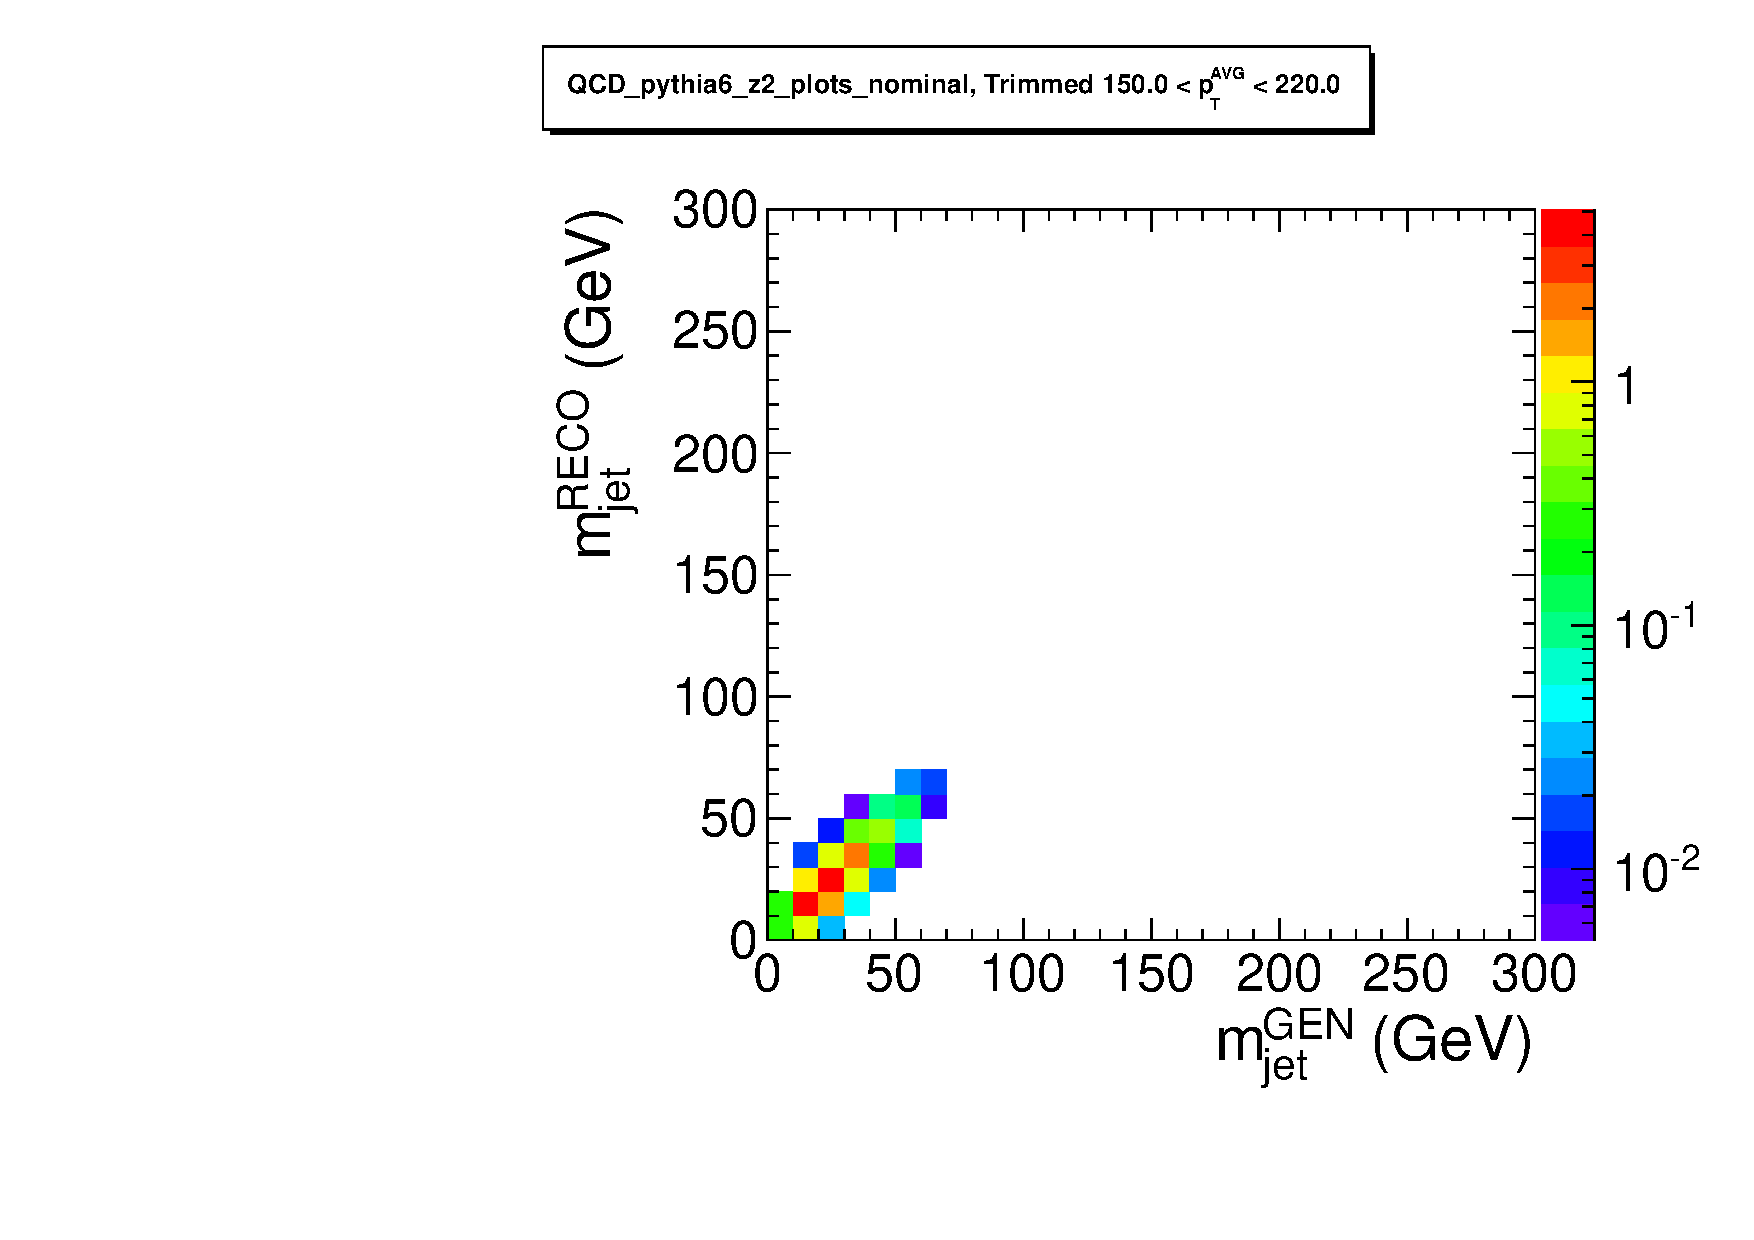
\includegraphics[width=0.3\textwidth]{figs/response_QCD_pythia6_z2_plots_nominal_Trimmed_pt3}}\\
\subfigure{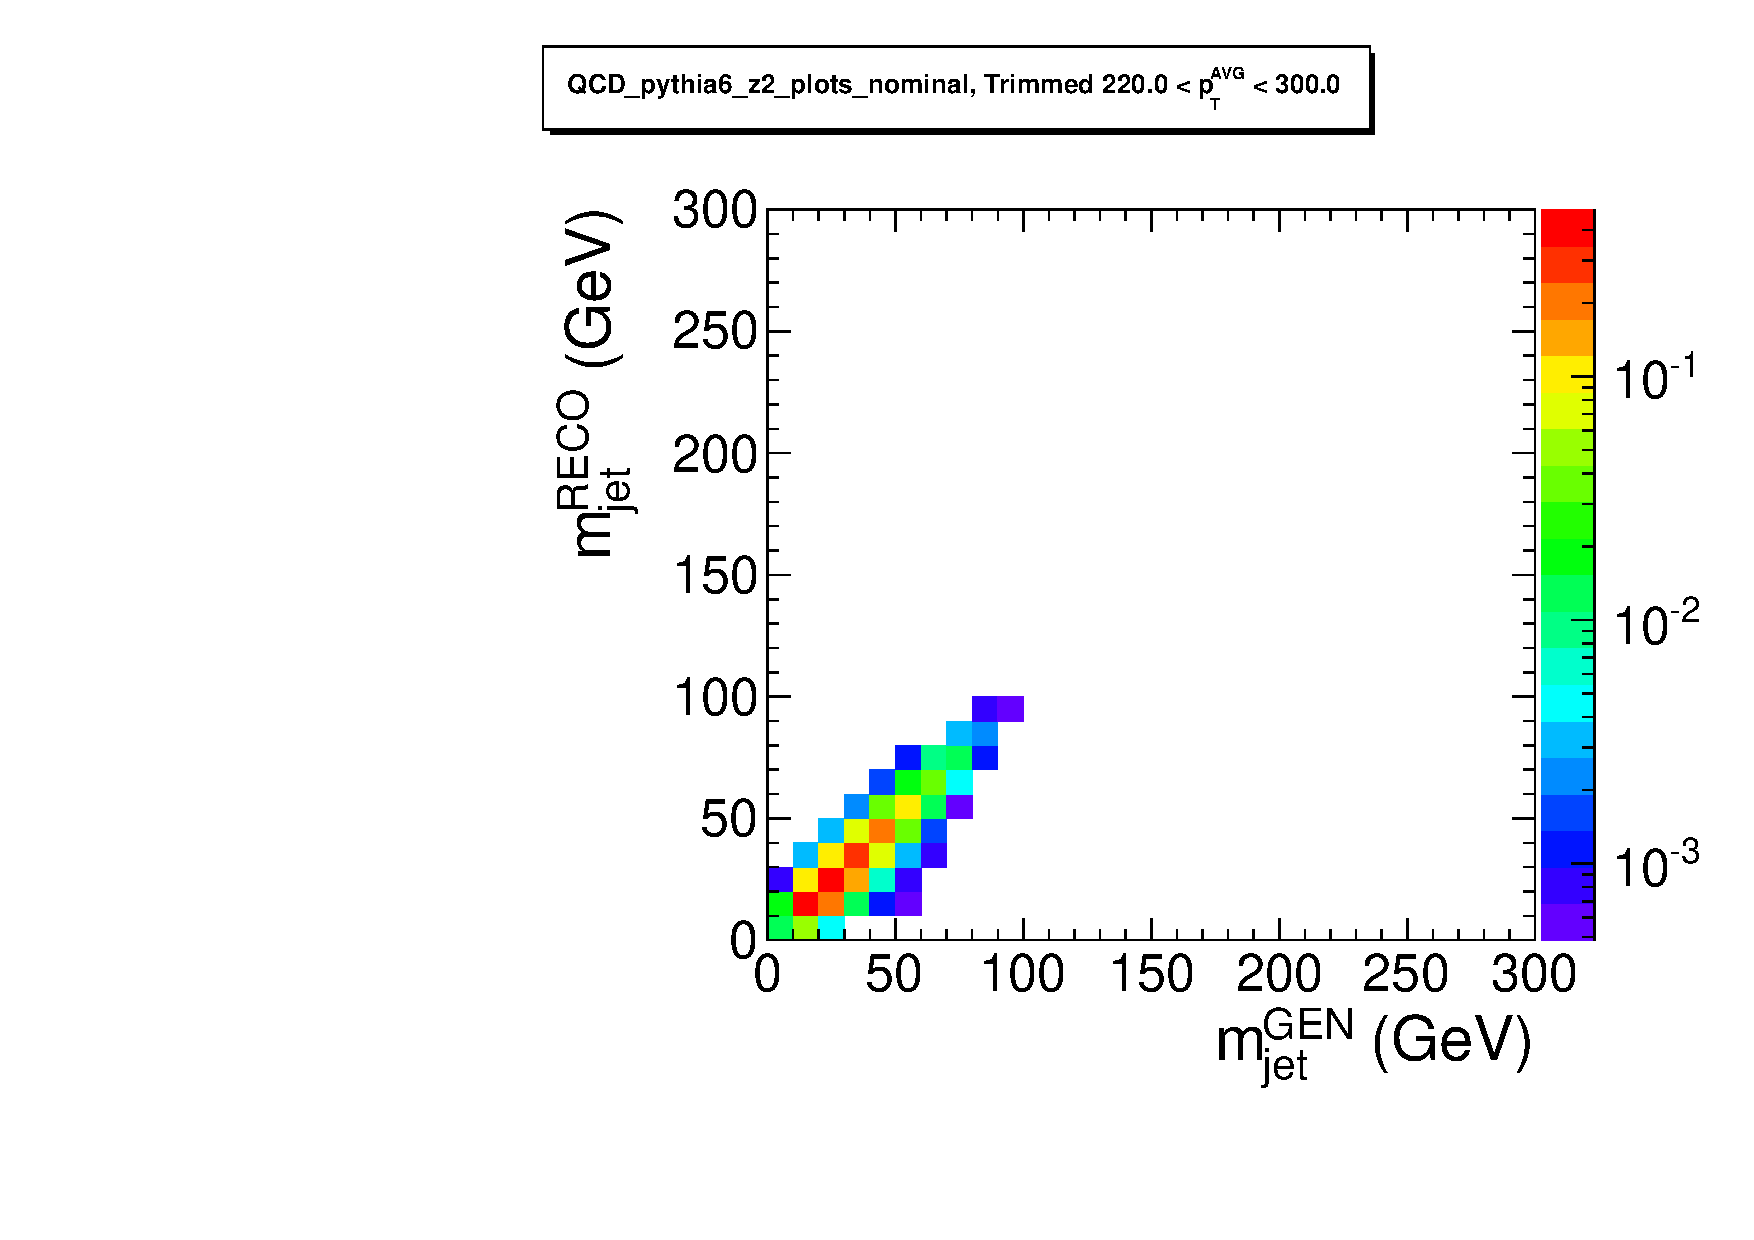
\includegraphics[width=0.3\textwidth]{figs/response_QCD_pythia6_z2_plots_nominal_Trimmed_pt4}}
\subfigure{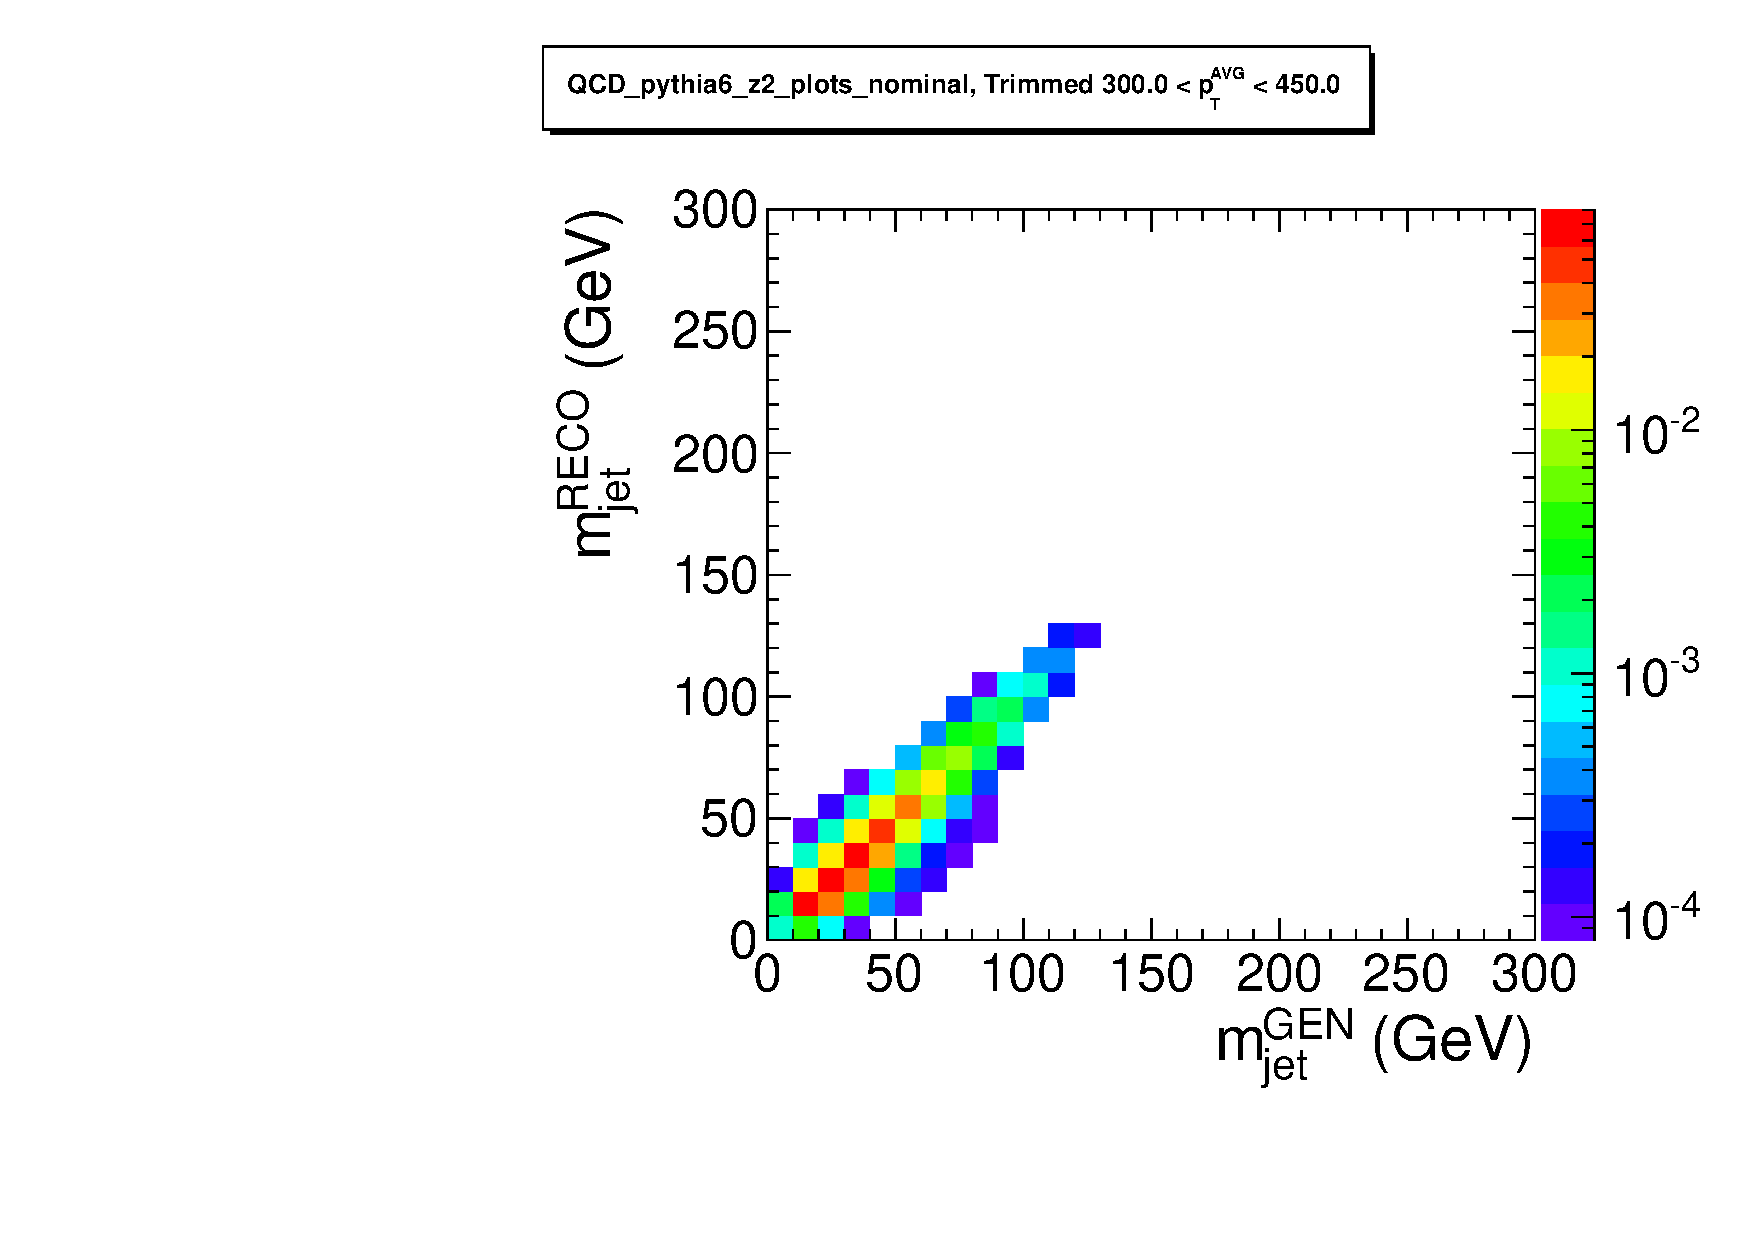
\includegraphics[width=0.3\textwidth]{figs/response_QCD_pythia6_z2_plots_nominal_Trimmed_pt5}}
\subfigure{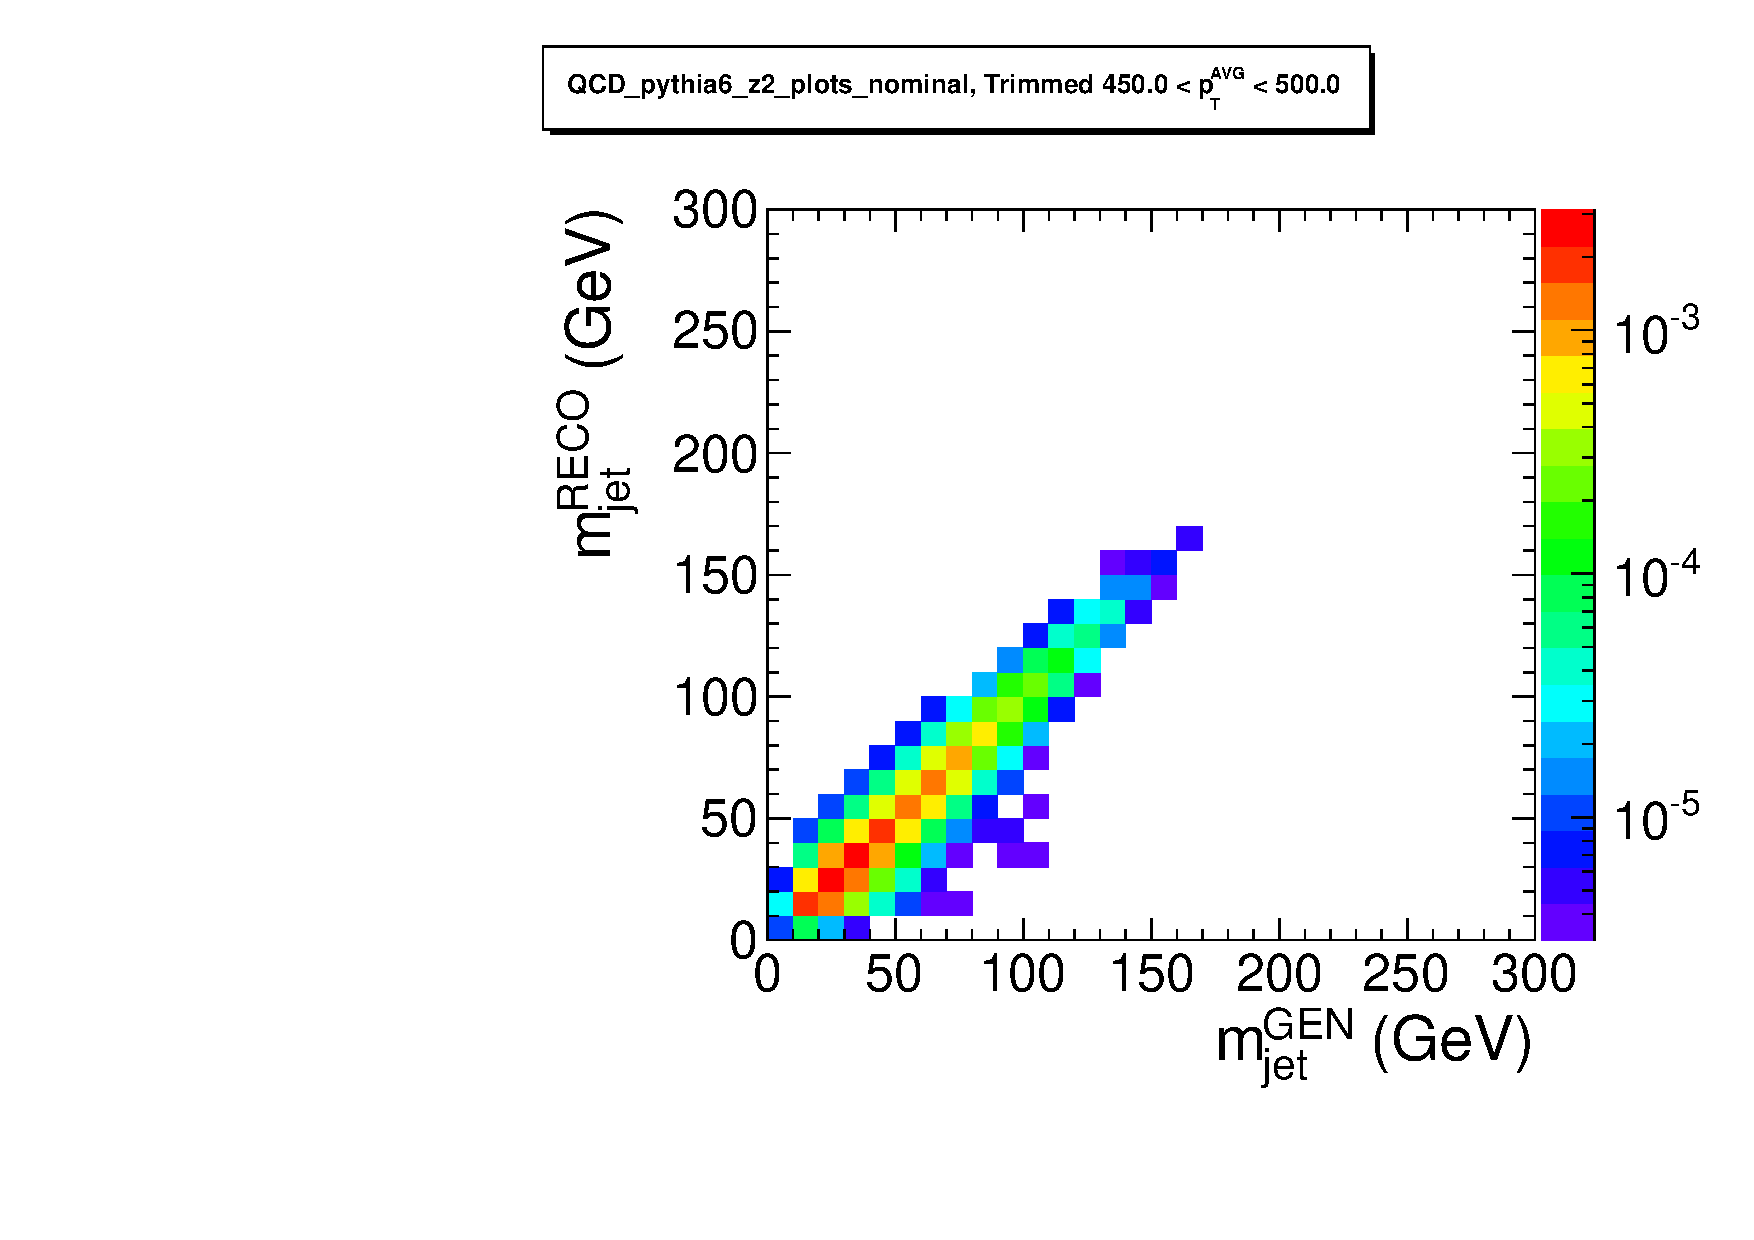
\includegraphics[width=0.3\textwidth]{figs/response_QCD_pythia6_z2_plots_nominal_Trimmed_pt6}}\\
\subfigure{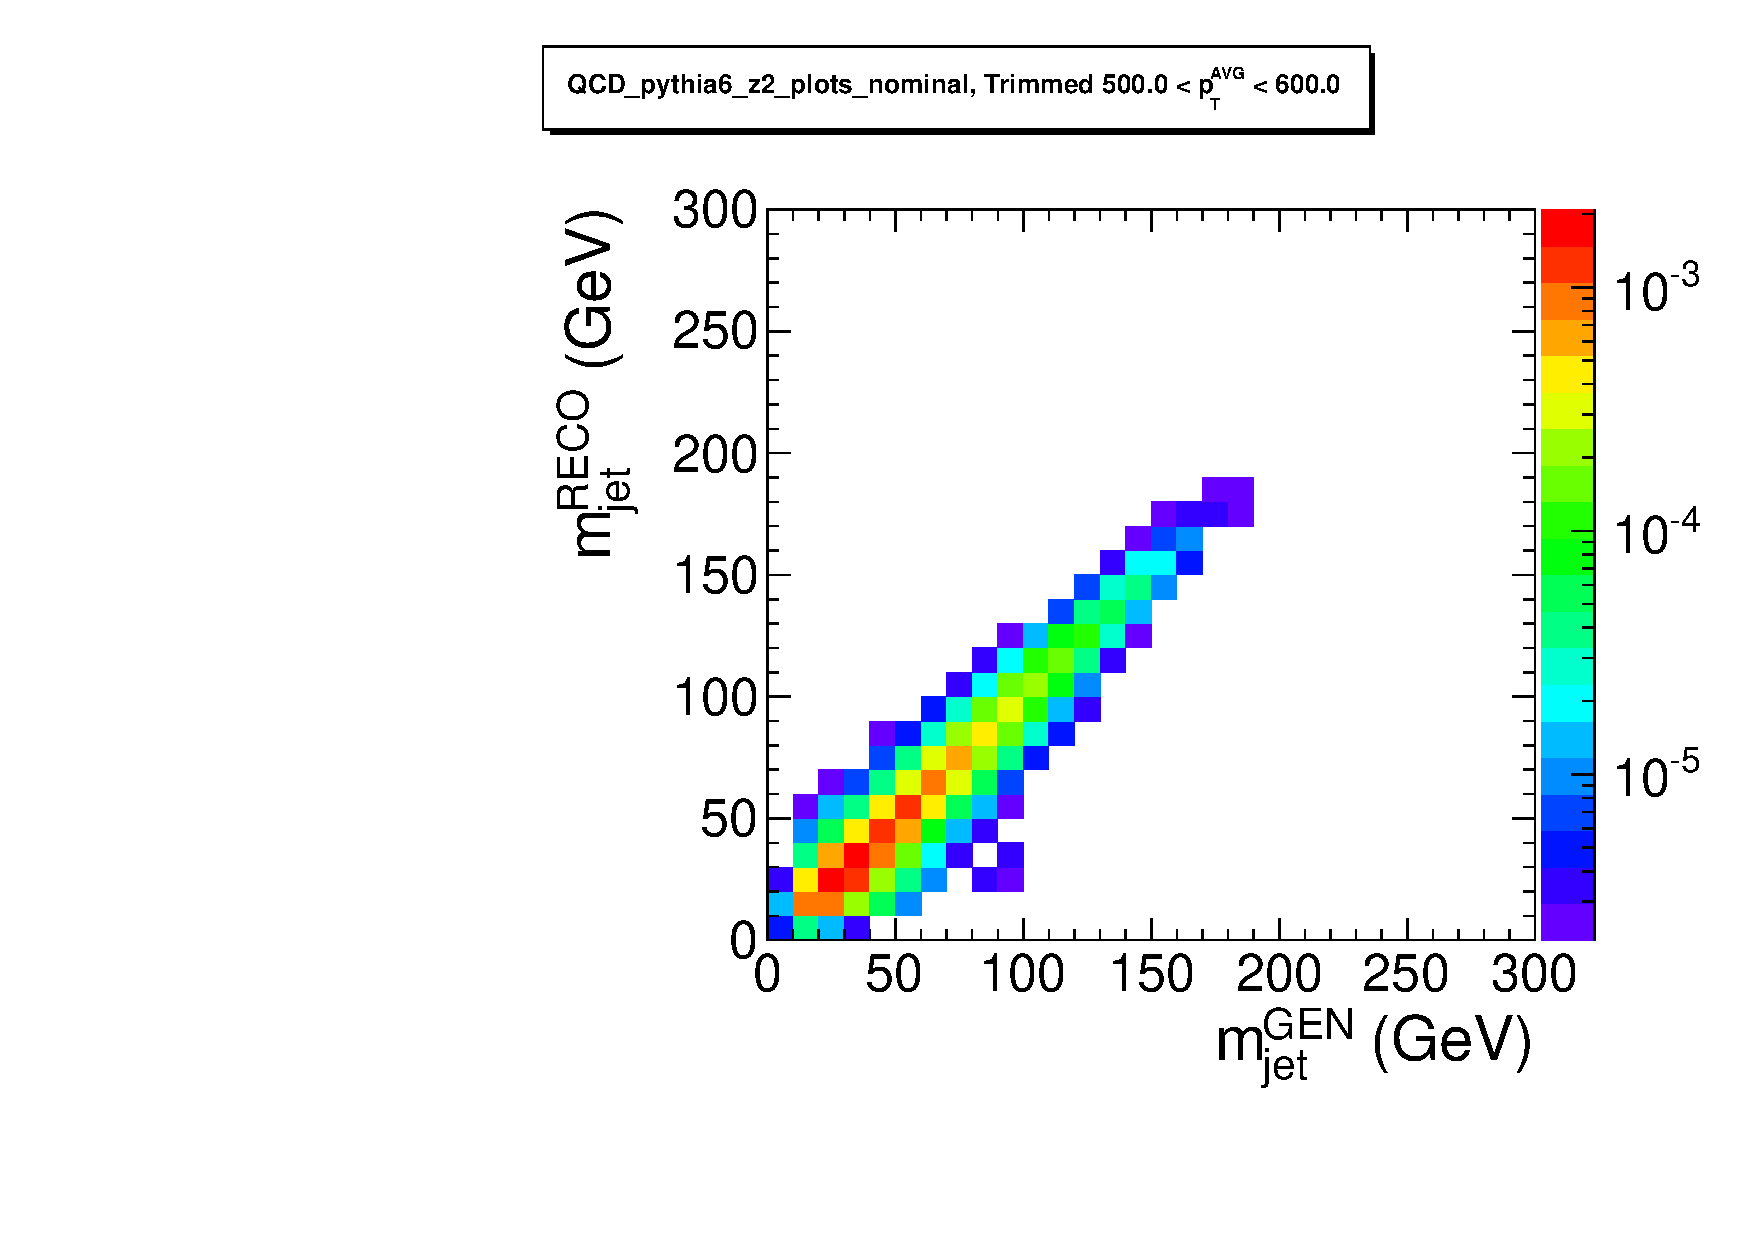
\includegraphics[width=0.3\textwidth]{figs/response_QCD_pythia6_z2_plots_nominal_Trimmed_pt7}}
\subfigure{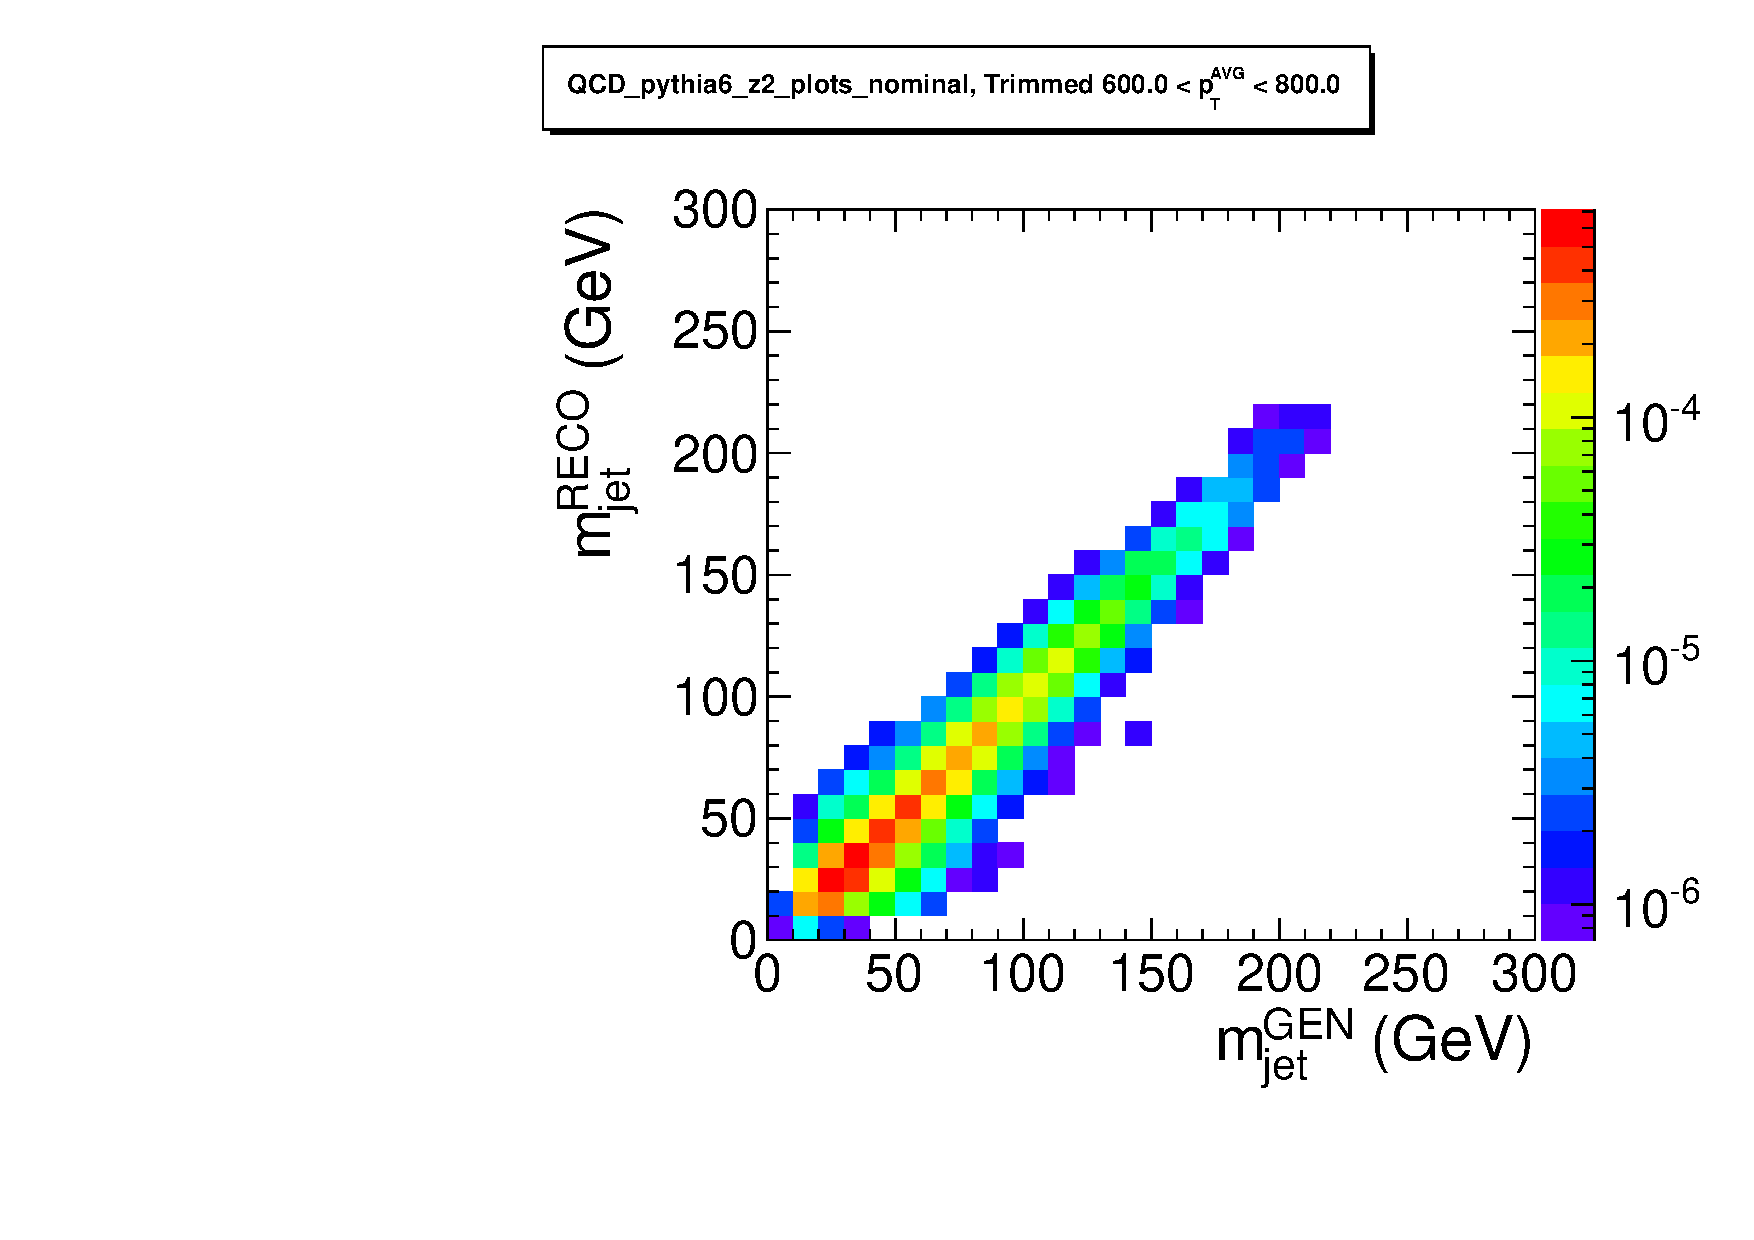
\includegraphics[width=0.3\textwidth]{figs/response_QCD_pythia6_z2_plots_nominal_Trimmed_pt8}}
\subfigure{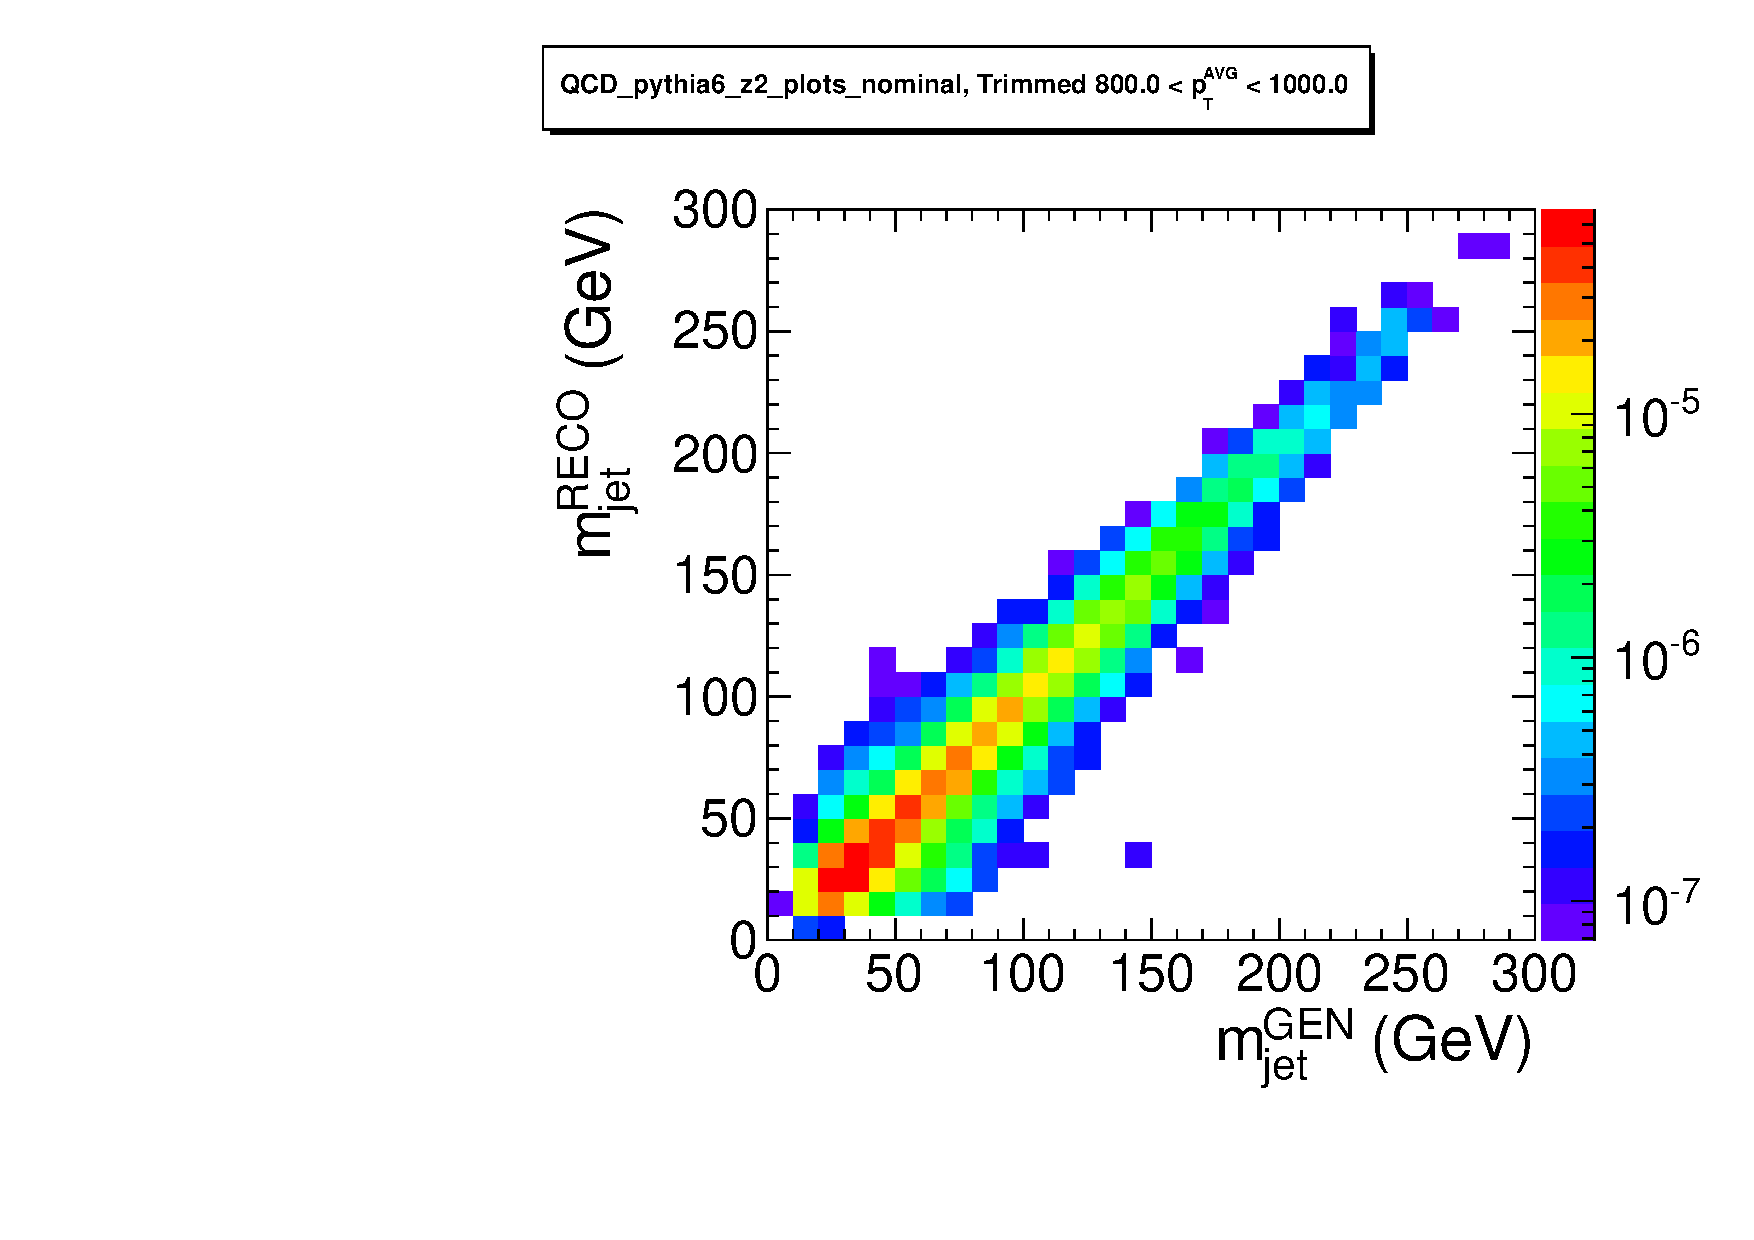
\includegraphics[width=0.3\textwidth]{figs/response_QCD_pythia6_z2_plots_nominal_Trimmed_pt9}}\\
\caption{Response of the jet mass for AK7 Trimmedjets,
for various $\pt^{AVG}$ bins. The true jet mass is shown
on the $x-$axis, and the reconstructed jet mass is shown on the
$y-$axis, using the \PYTHIA generator. 
\label{figs:response_QCD_pythia6_z2_plots_nominal_Trimmed_ptall}}
\end{figure}


\clearpage

\begin{figure}[htbp]
\centering
\subfigure{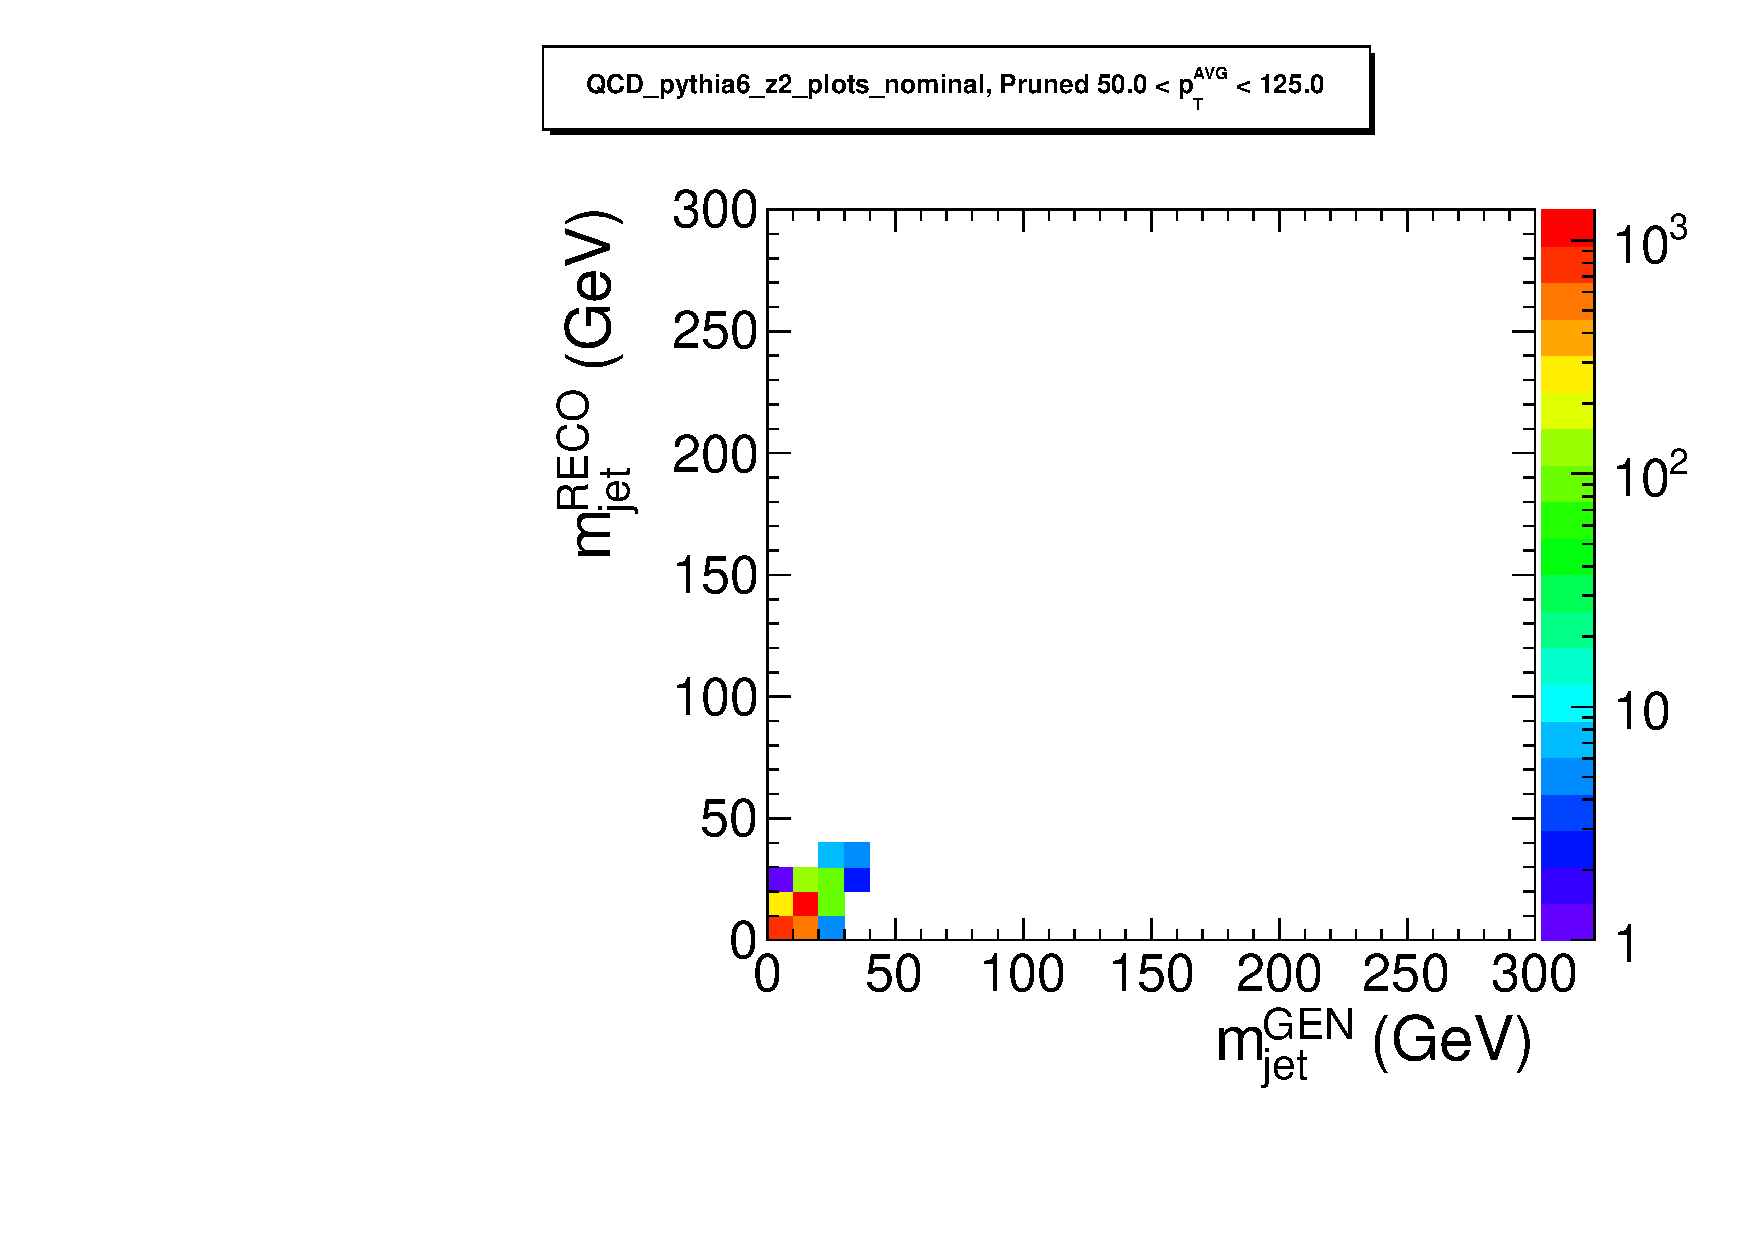
\includegraphics[width=0.3\textwidth]{figs/response_QCD_pythia6_z2_plots_nominal_Pruned_pt1}}
\subfigure{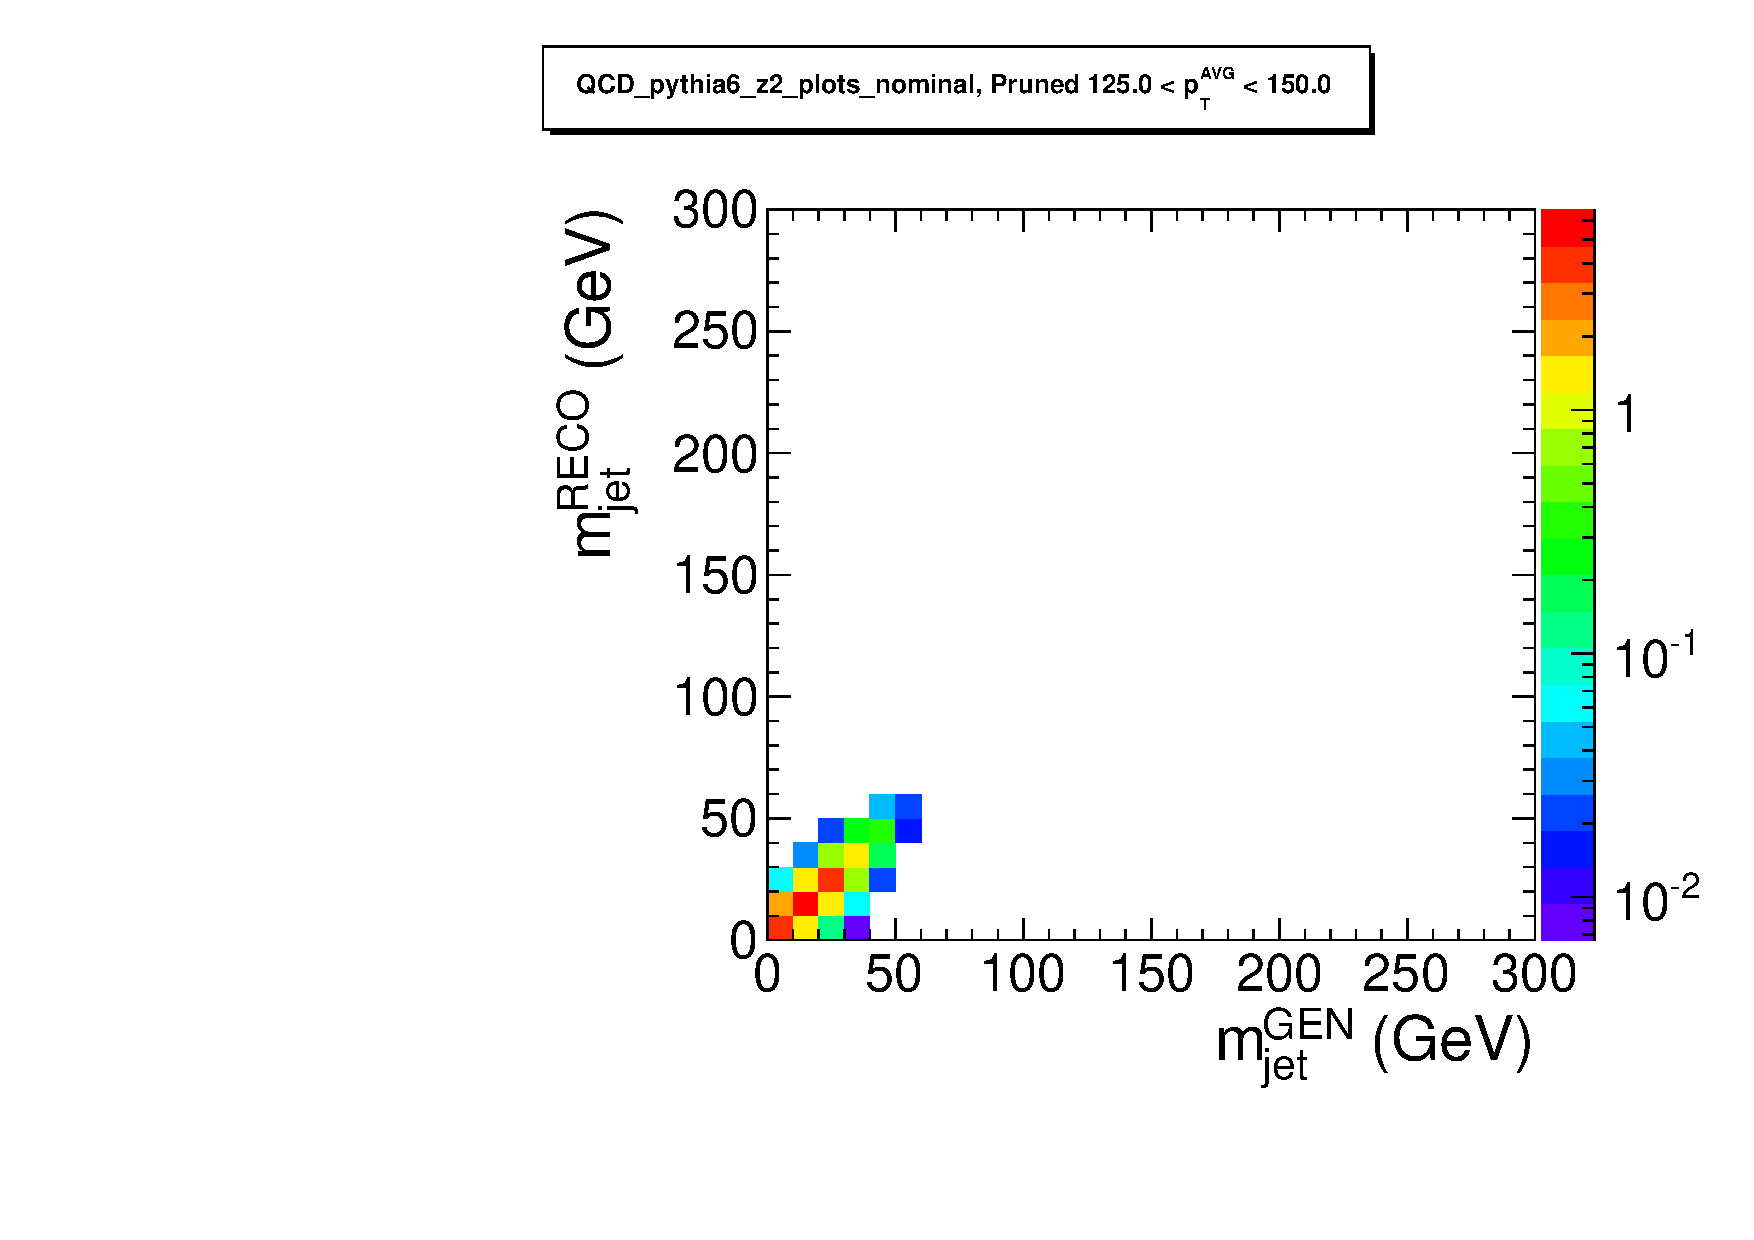
\includegraphics[width=0.3\textwidth]{figs/response_QCD_pythia6_z2_plots_nominal_Pruned_pt2}}
\subfigure{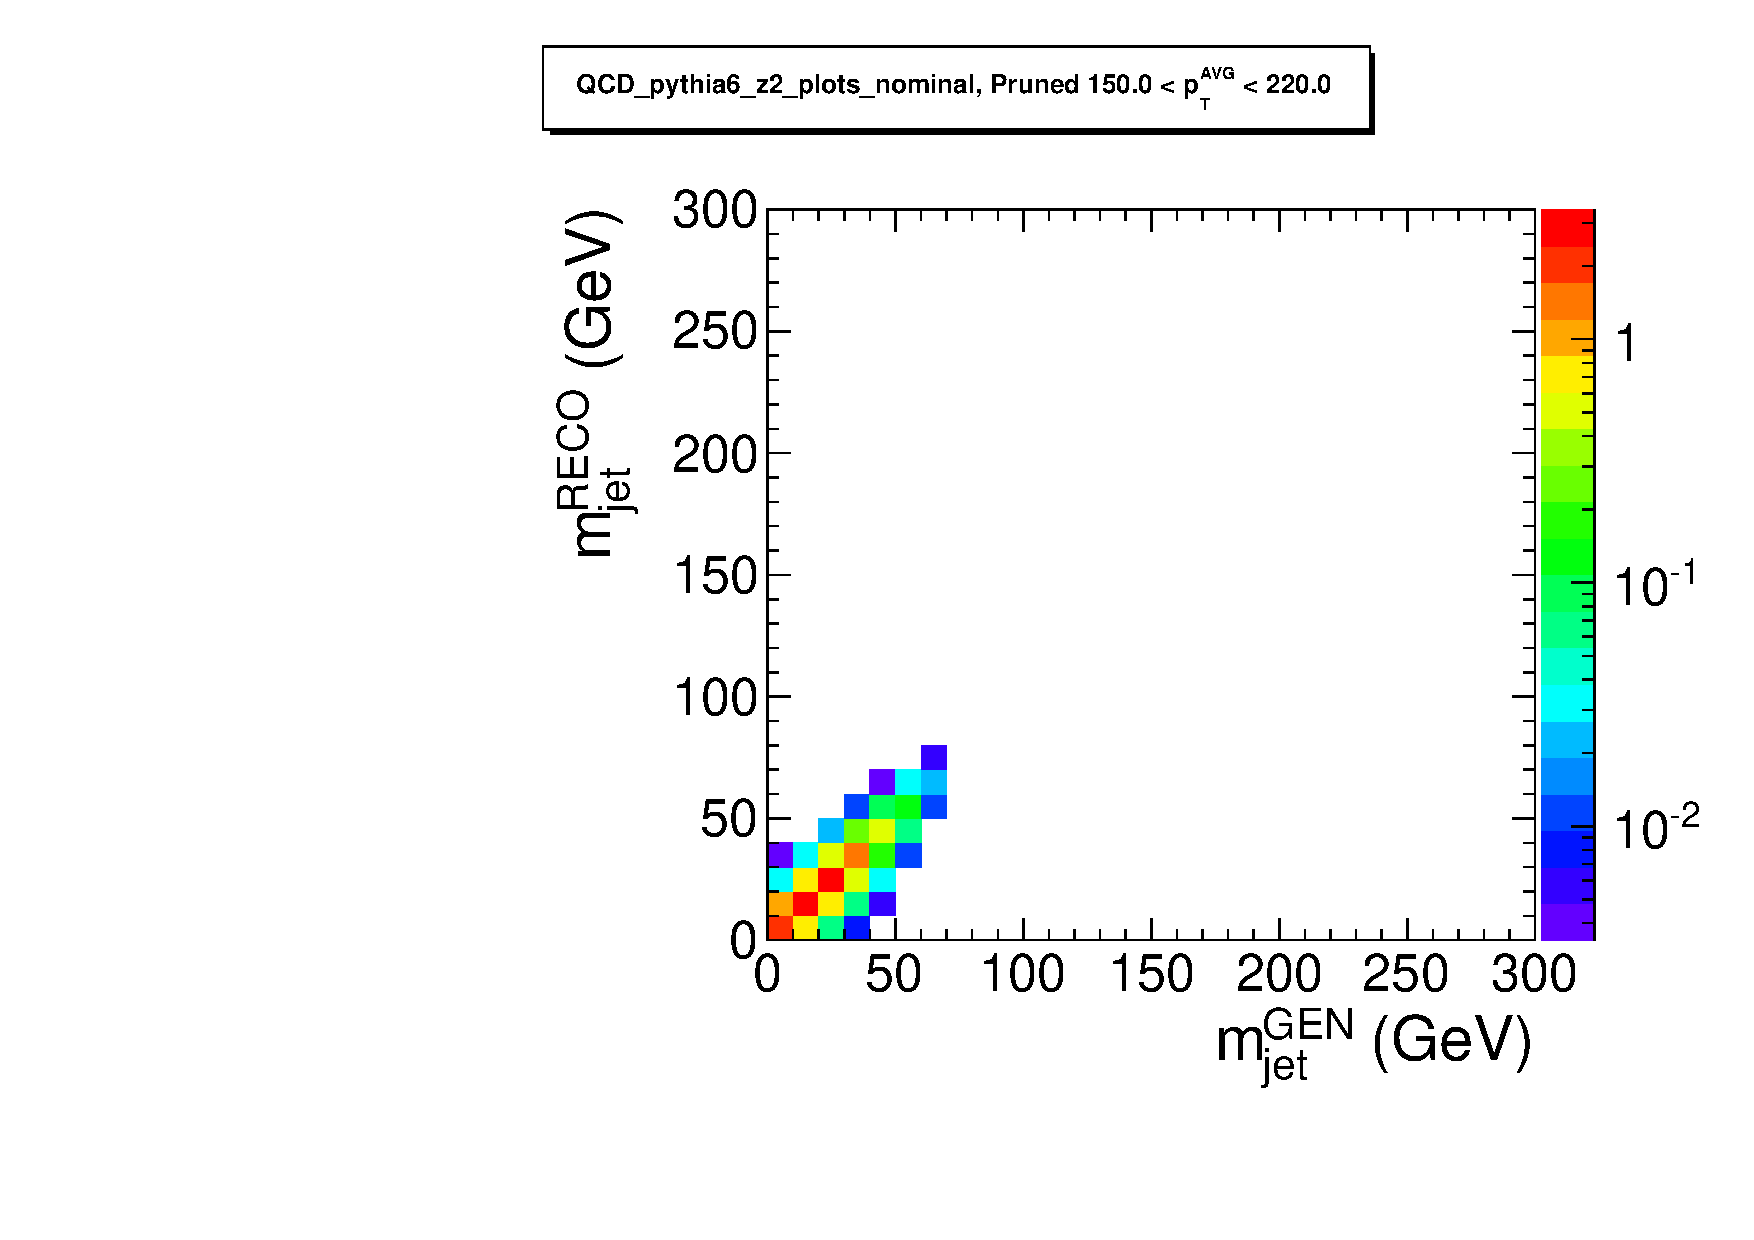
\includegraphics[width=0.3\textwidth]{figs/response_QCD_pythia6_z2_plots_nominal_Pruned_pt3}}\\
\subfigure{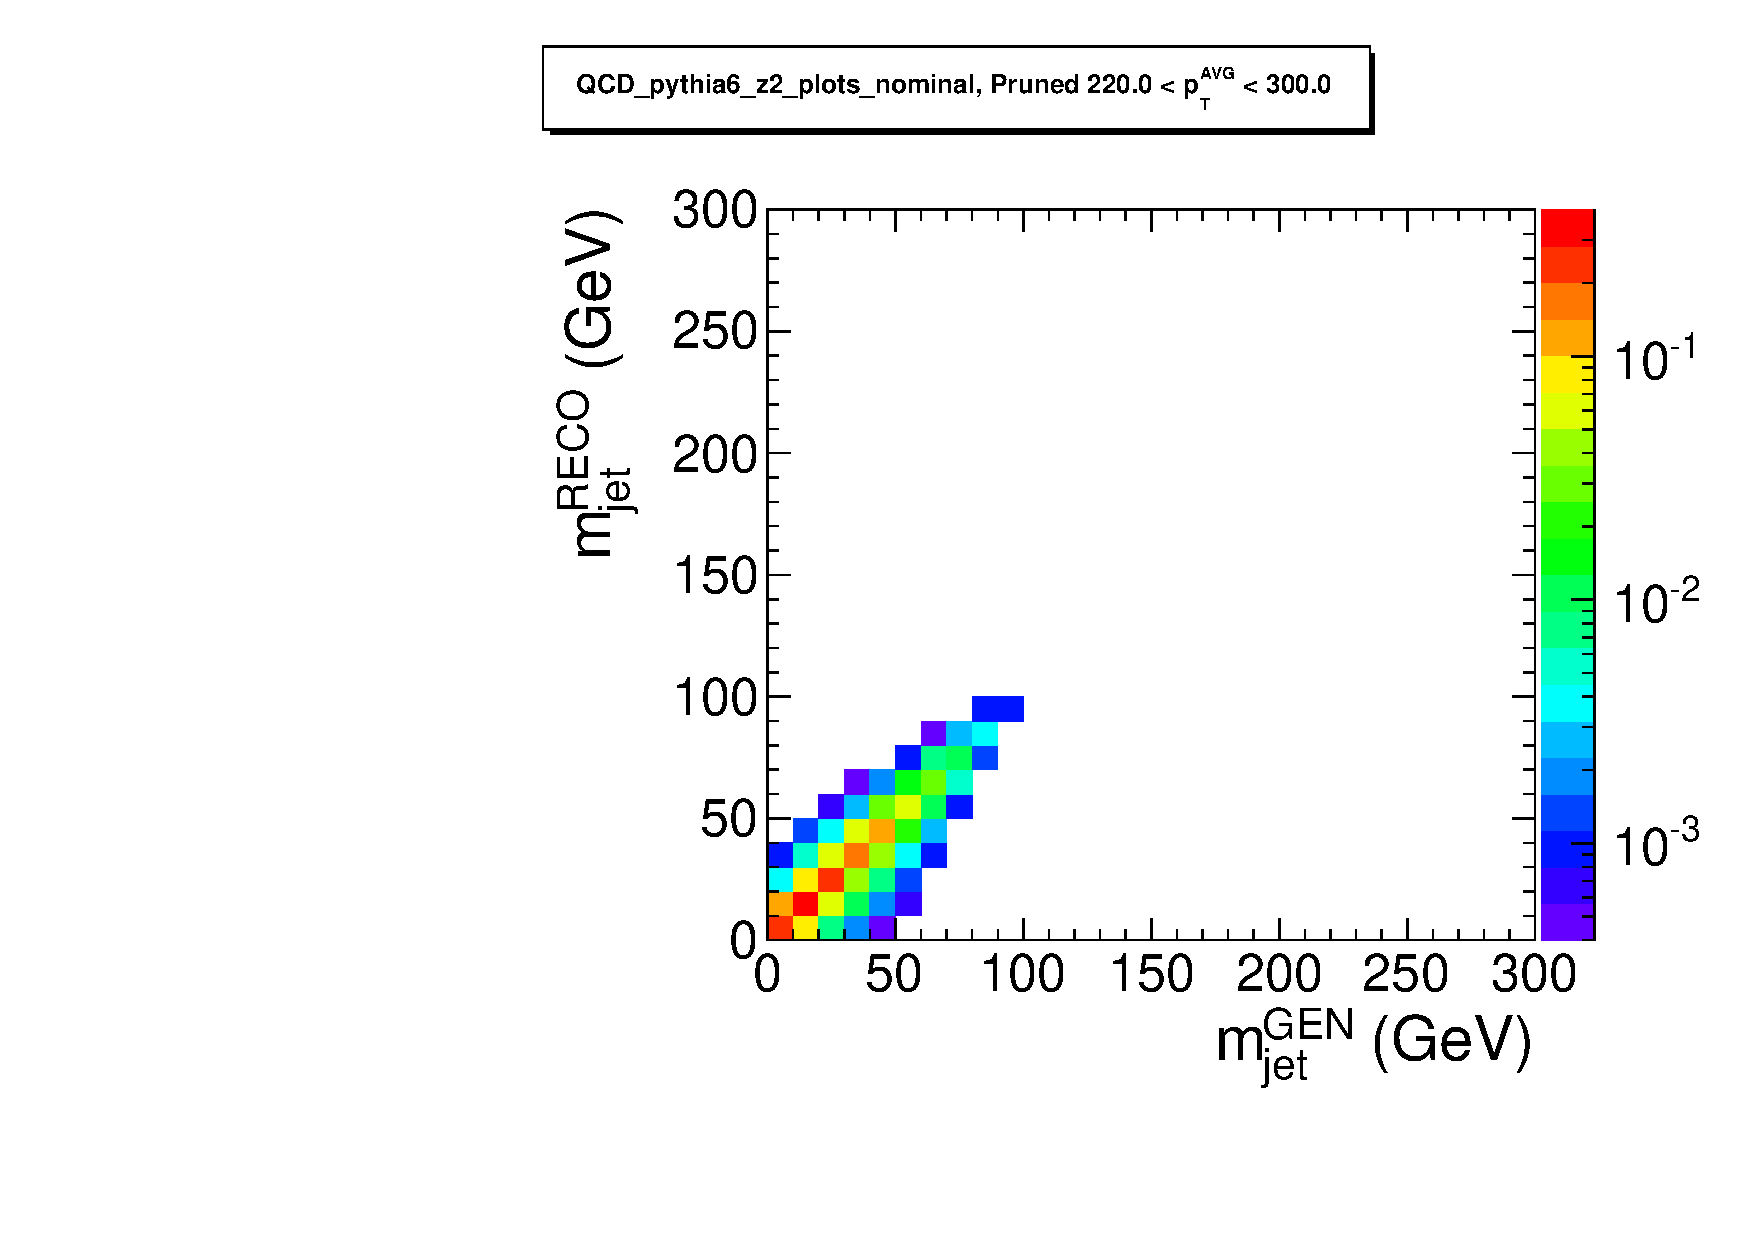
\includegraphics[width=0.3\textwidth]{figs/response_QCD_pythia6_z2_plots_nominal_Pruned_pt4}}
\subfigure{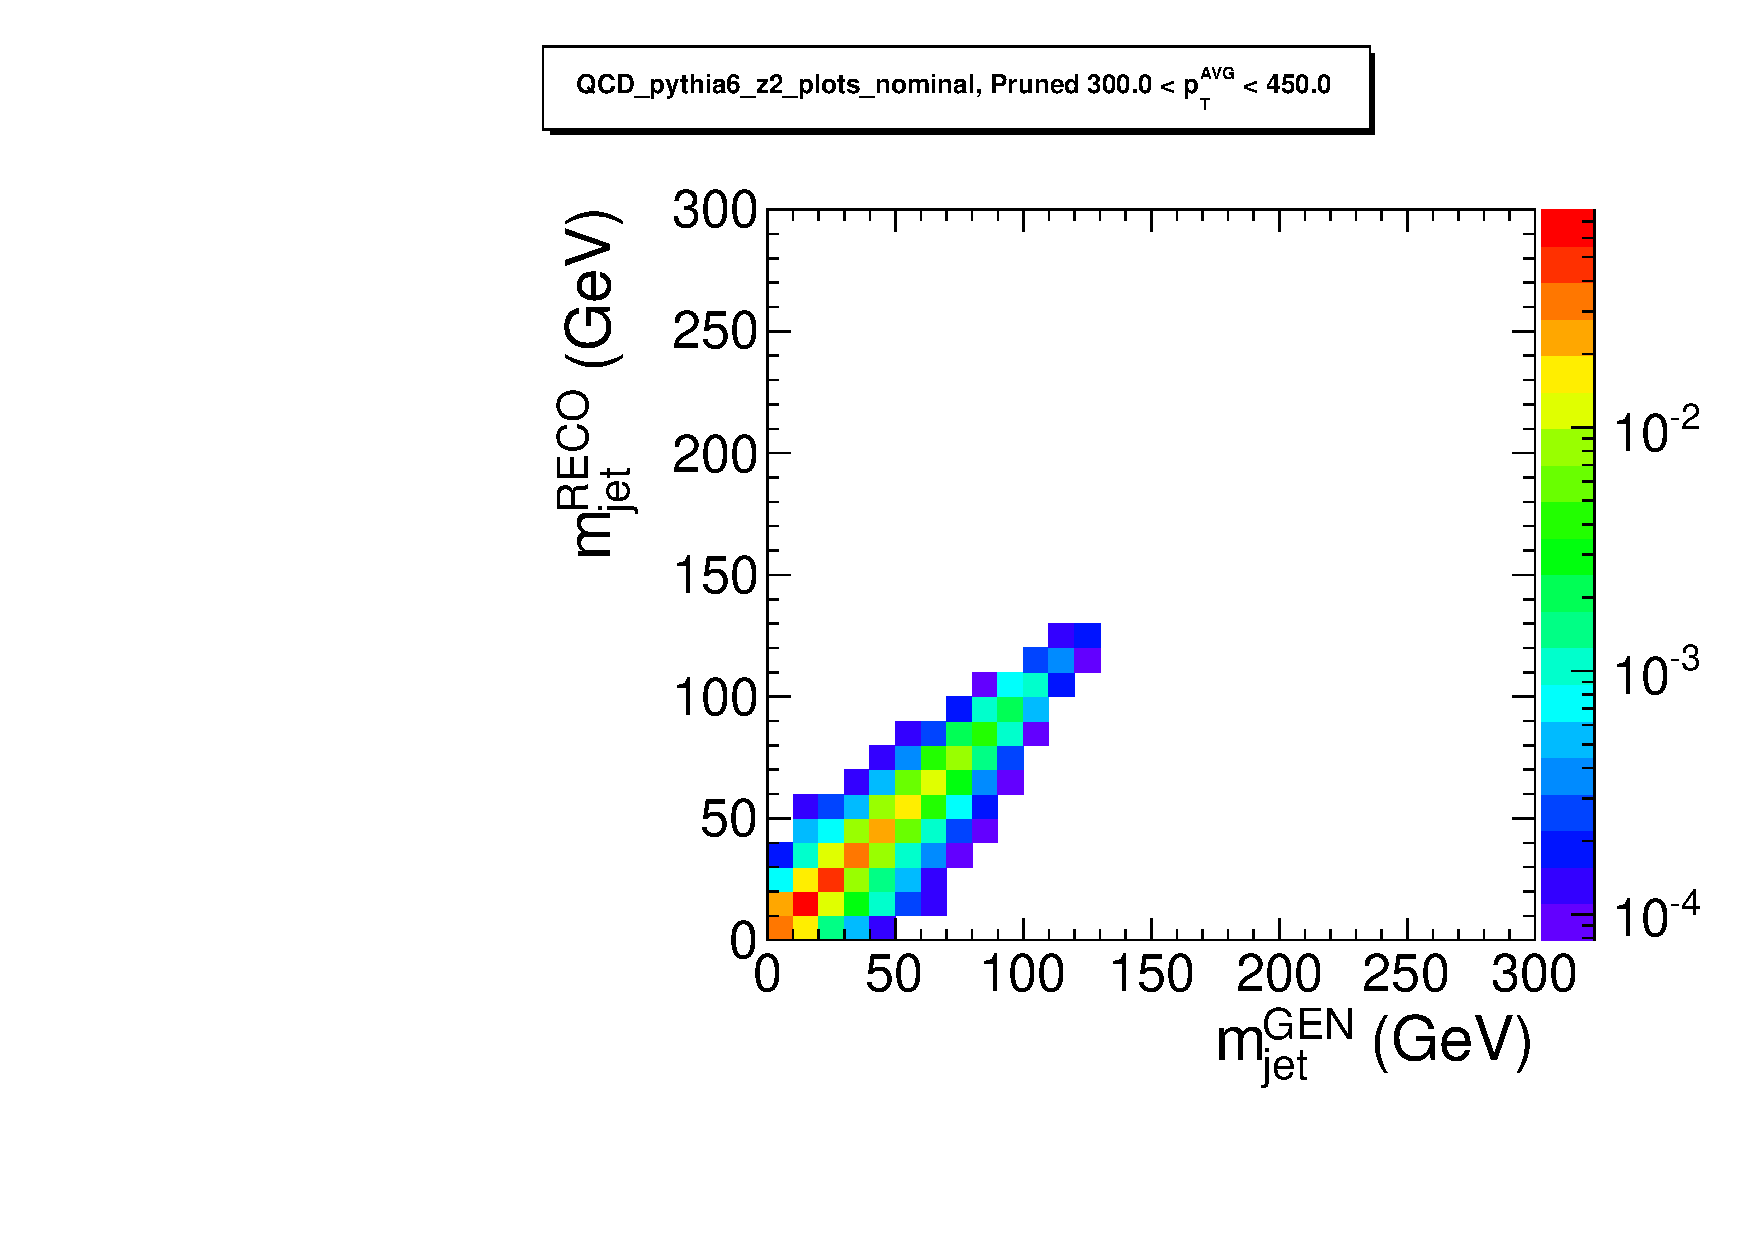
\includegraphics[width=0.3\textwidth]{figs/response_QCD_pythia6_z2_plots_nominal_Pruned_pt5}}
\subfigure{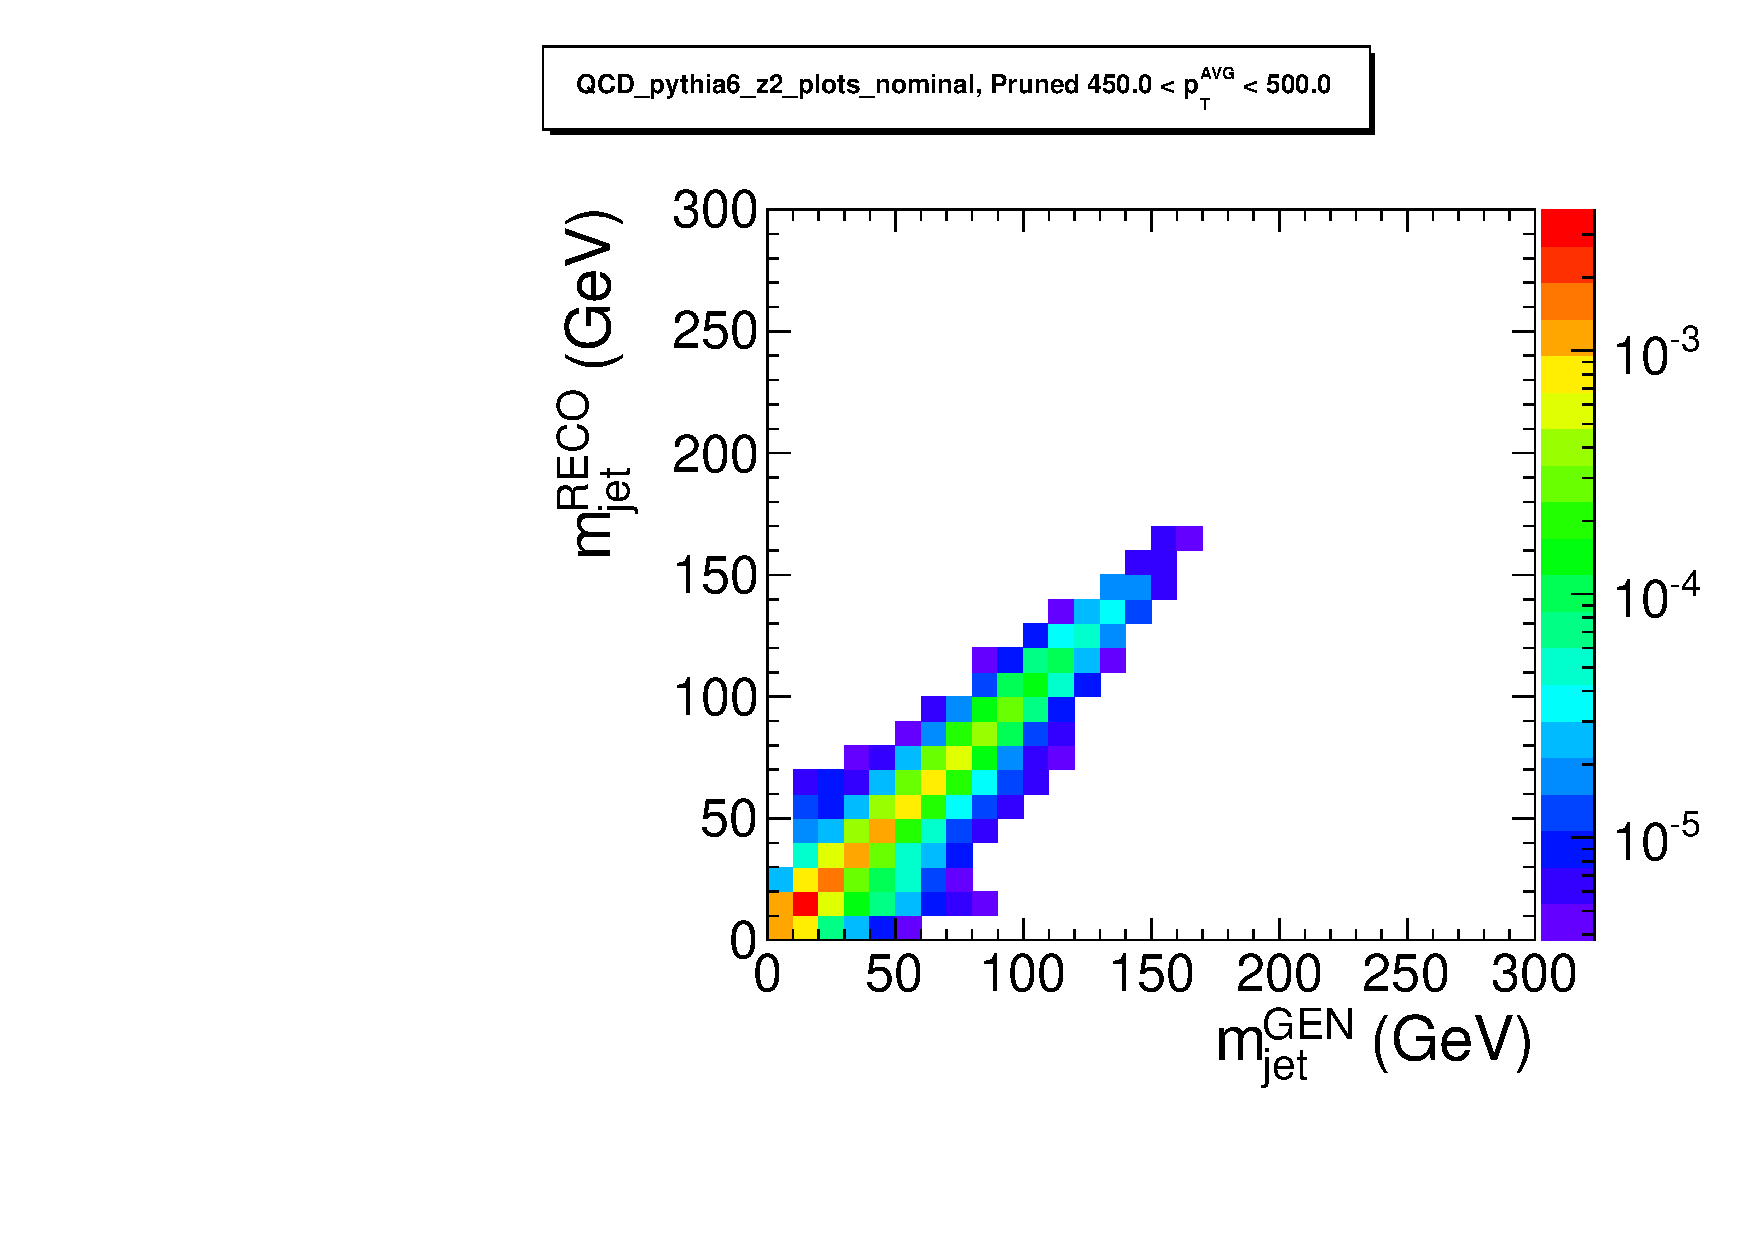
\includegraphics[width=0.3\textwidth]{figs/response_QCD_pythia6_z2_plots_nominal_Pruned_pt6}}\\
\subfigure{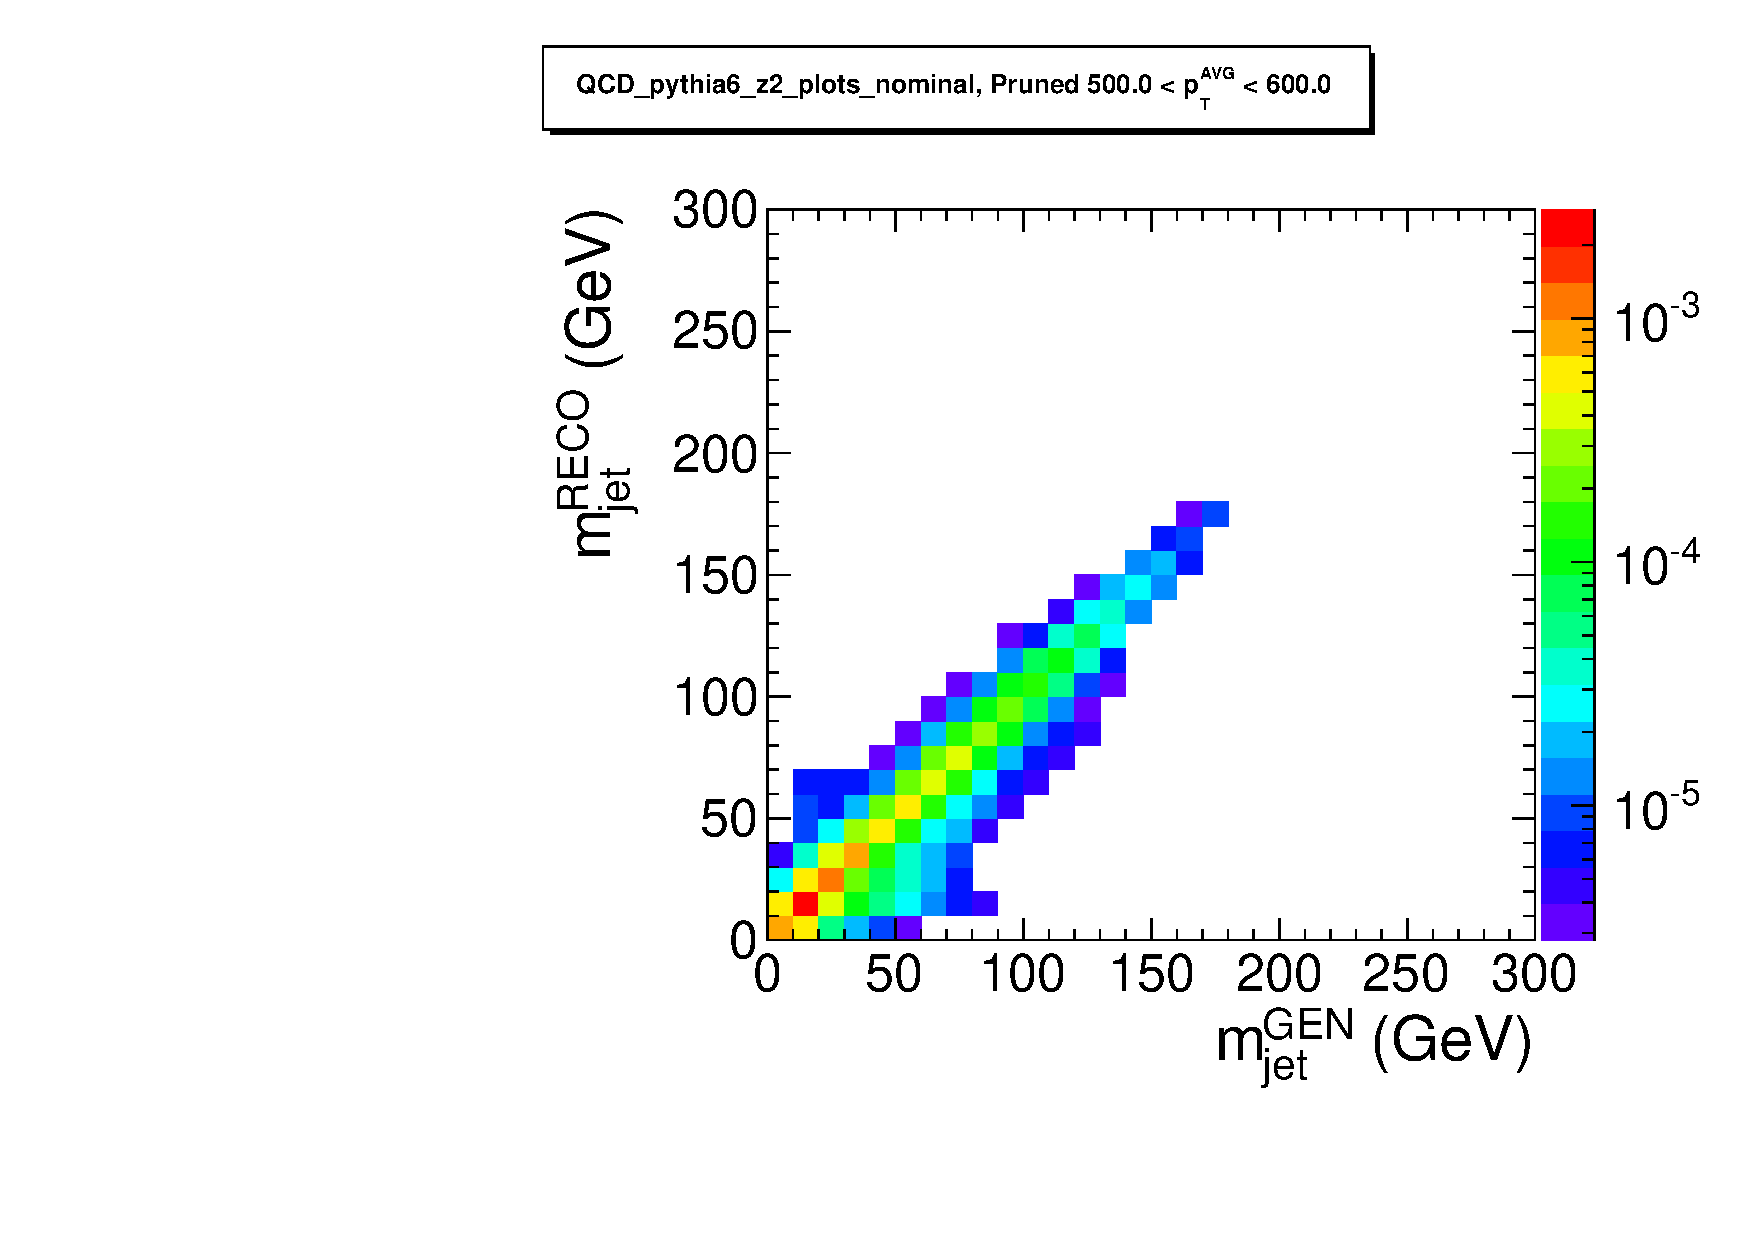
\includegraphics[width=0.3\textwidth]{figs/response_QCD_pythia6_z2_plots_nominal_Pruned_pt7}}
\subfigure{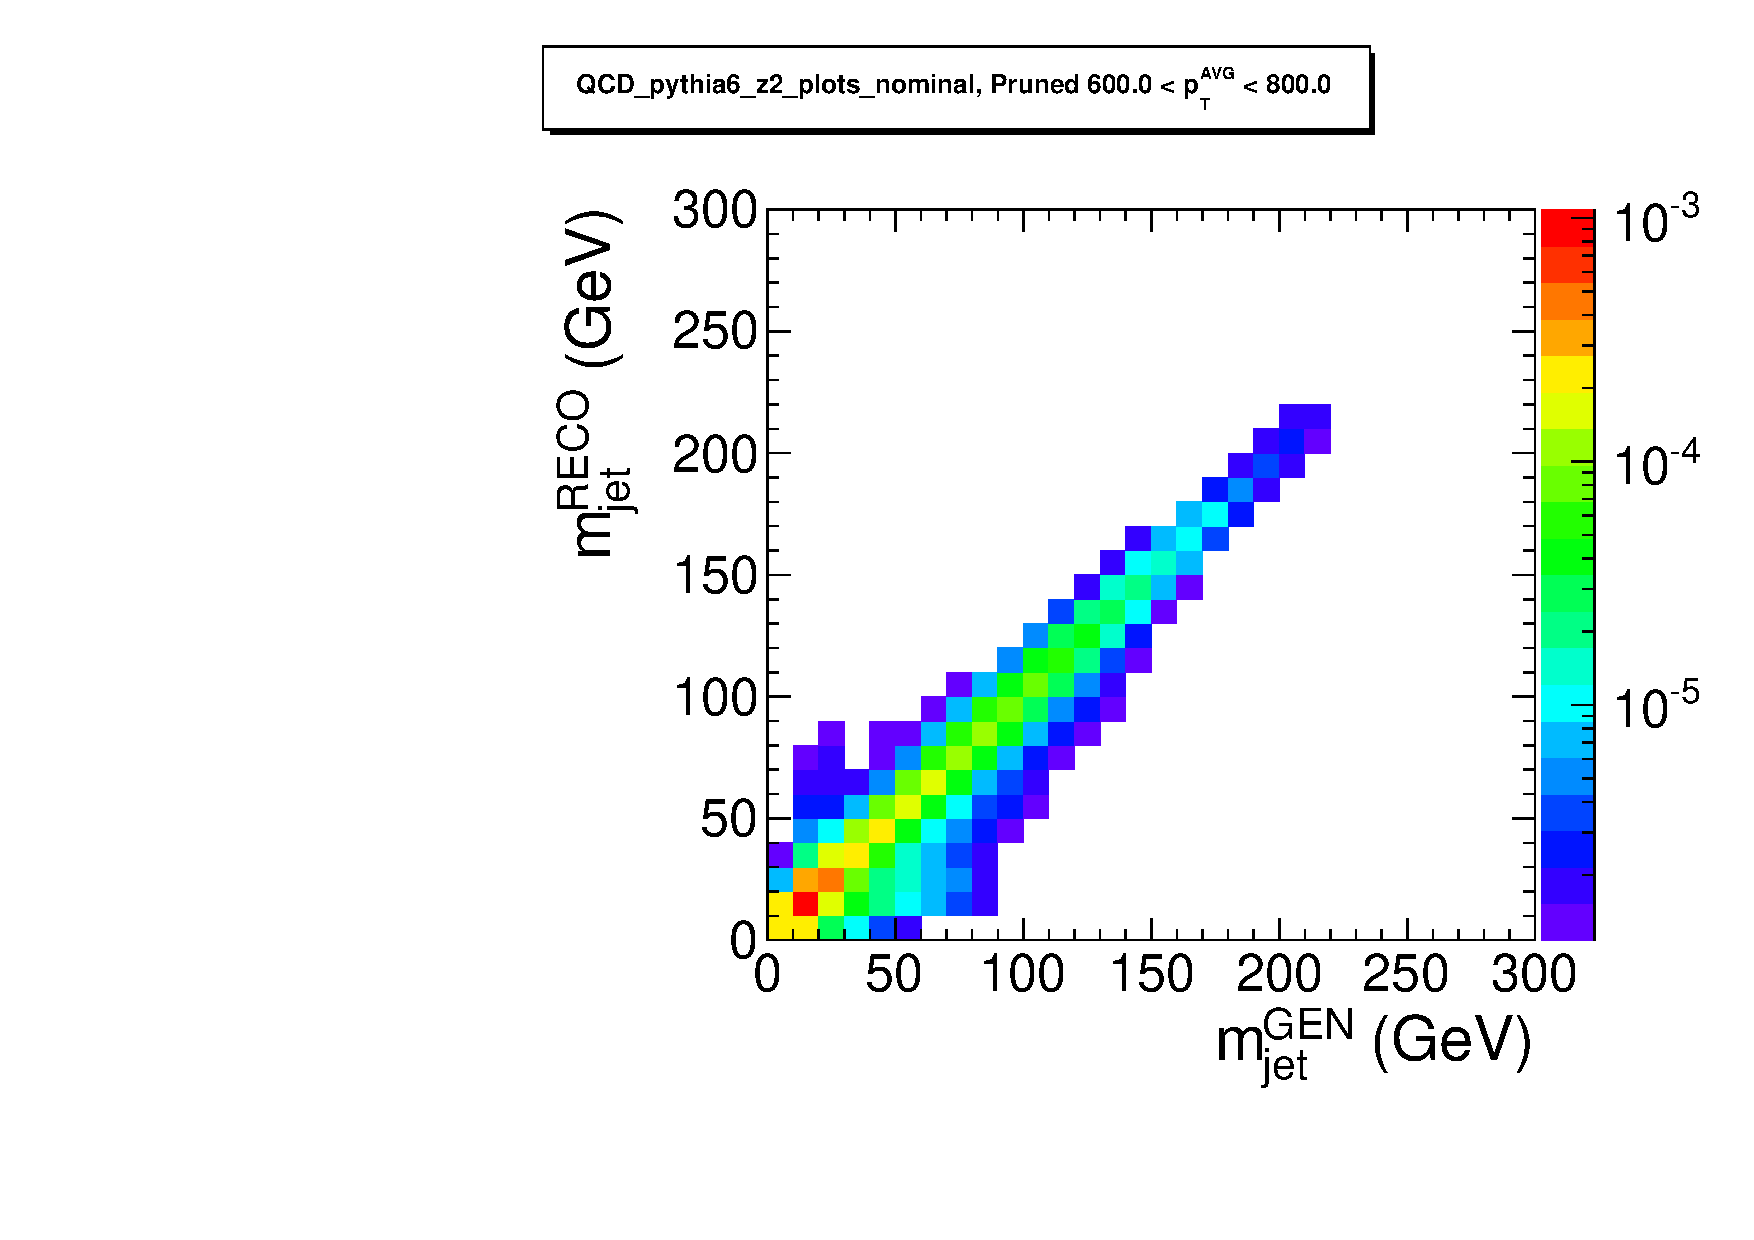
\includegraphics[width=0.3\textwidth]{figs/response_QCD_pythia6_z2_plots_nominal_Pruned_pt8}}
\subfigure{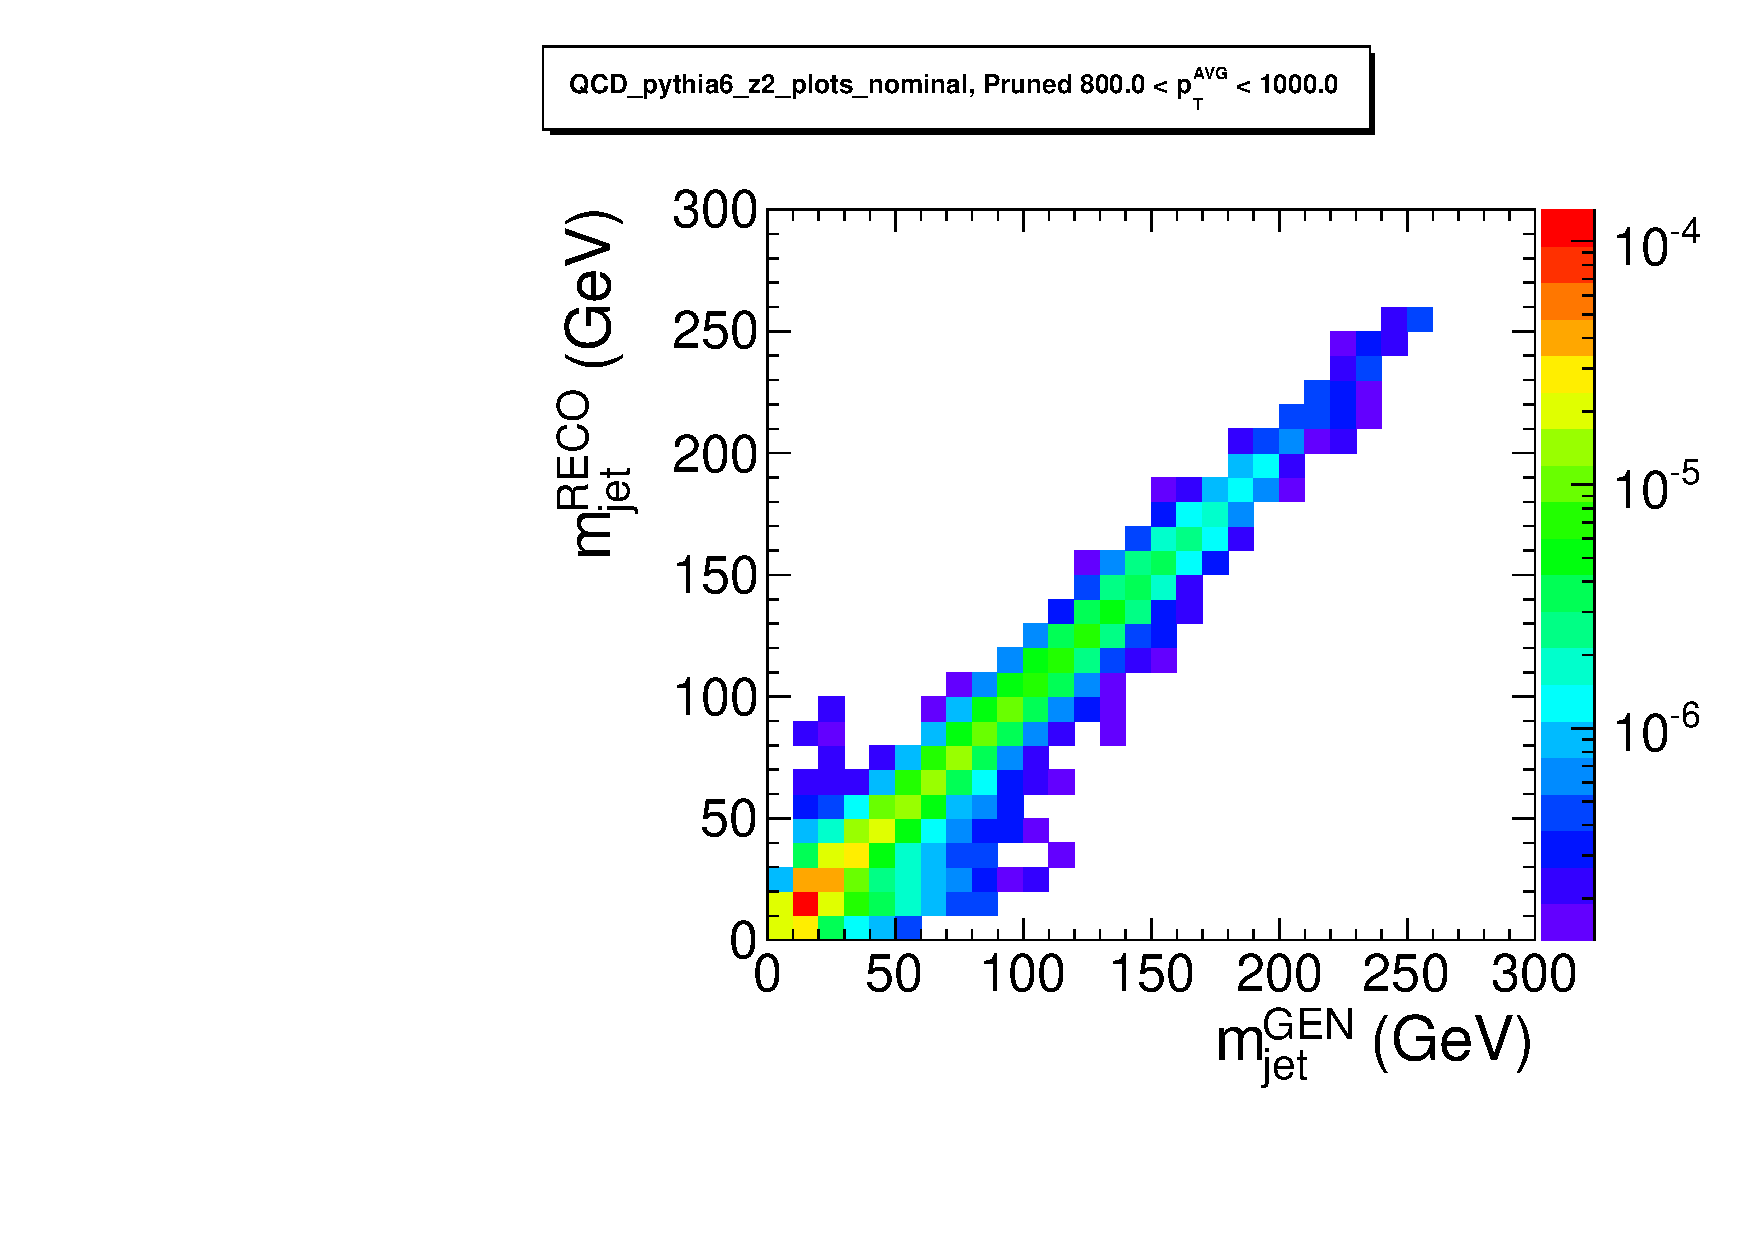
\includegraphics[width=0.3\textwidth]{figs/response_QCD_pythia6_z2_plots_nominal_Pruned_pt9}}\\
\caption{Response of the jet mass for AK7 Prunedjets,
for various $\pt^{AVG}$ bins. The true jet mass is shown
on the $x-$axis, and the reconstructed jet mass is shown on the
$y-$axis, using the \PYTHIA generator. 
\label{figs:response_QCD_pythia6_z2_plots_nominal_Pruned_ptall}}
\end{figure}


\clearpage

\begin{figure}[htbp]
\centering
\subfigure{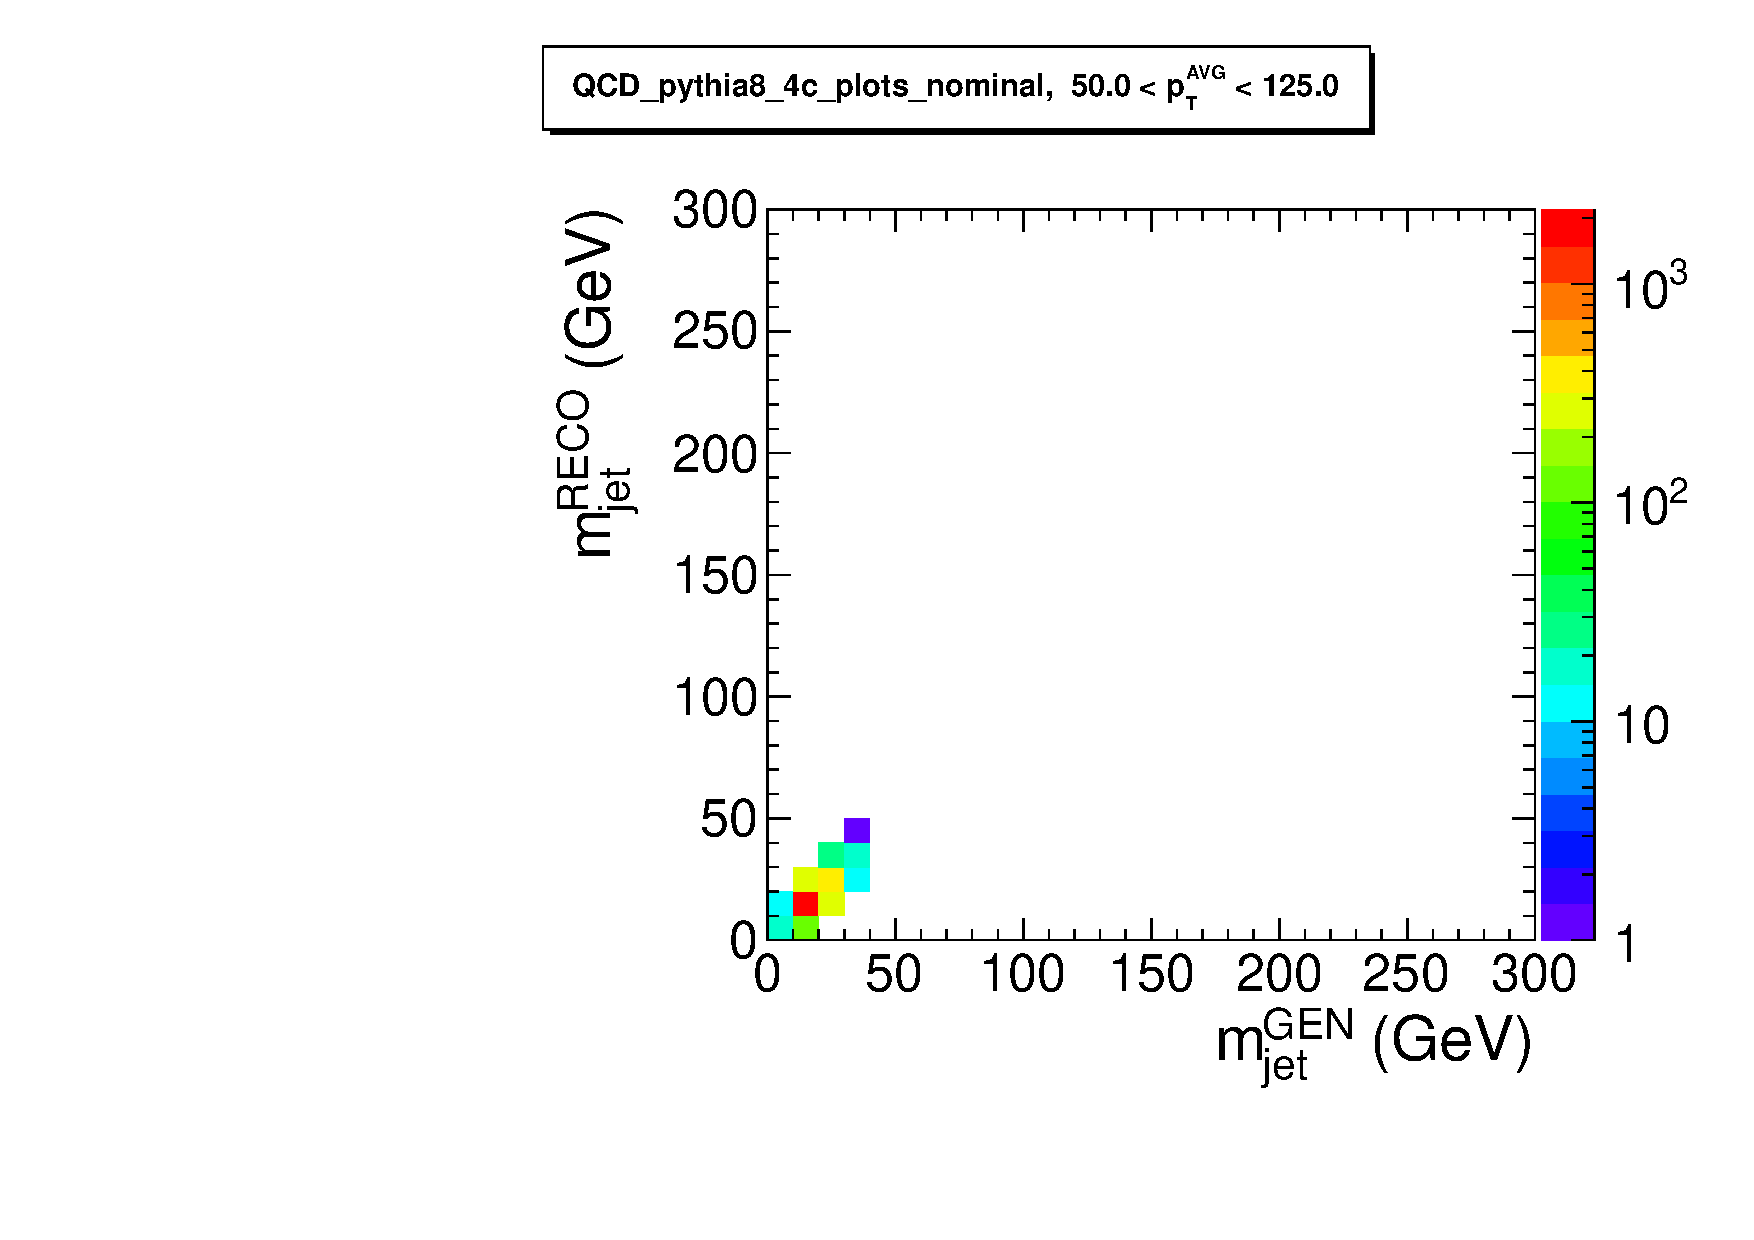
\includegraphics[width=0.3\textwidth]{figs/response_QCD_pythia8_4c_plots_nominal_pt1}}
\subfigure{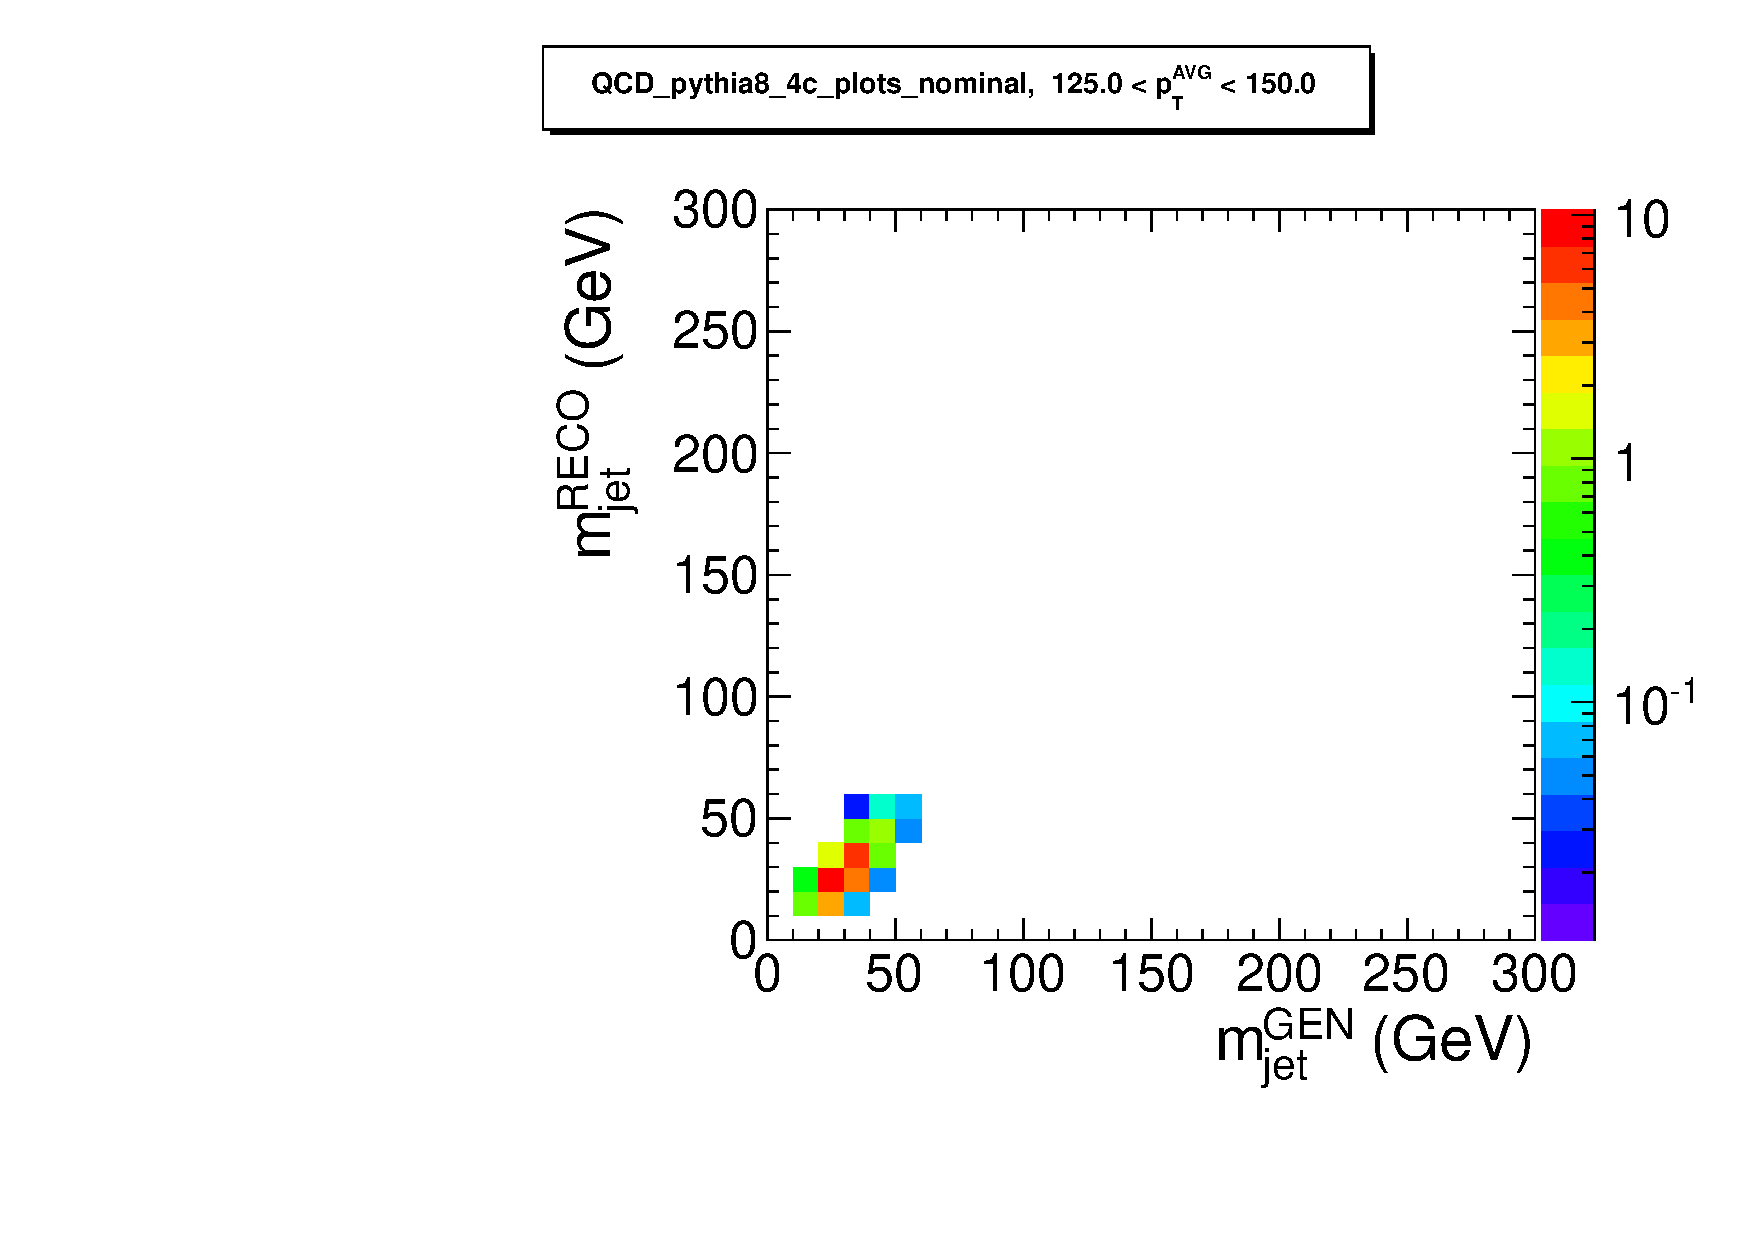
\includegraphics[width=0.3\textwidth]{figs/response_QCD_pythia8_4c_plots_nominal_pt2}}
\subfigure{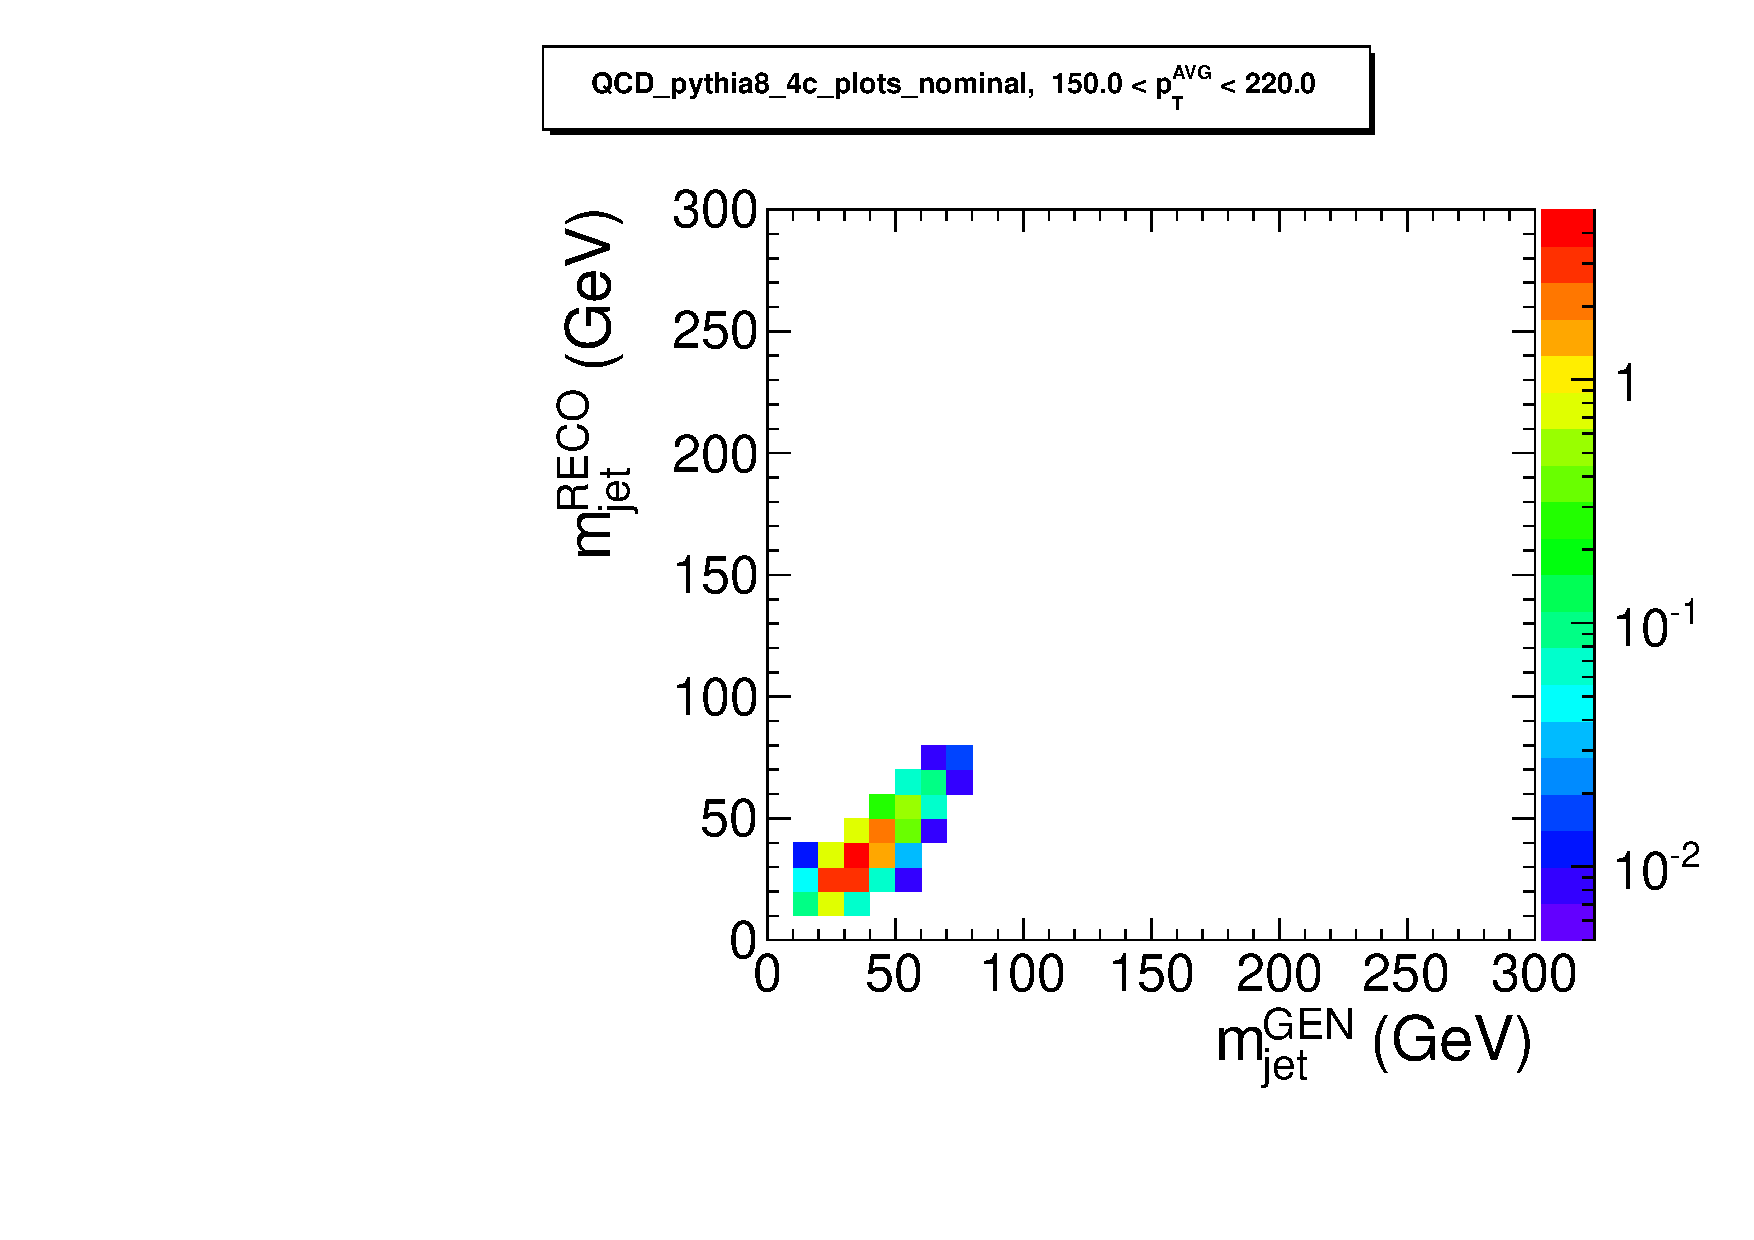
\includegraphics[width=0.3\textwidth]{figs/response_QCD_pythia8_4c_plots_nominal_pt3}}\\
\subfigure{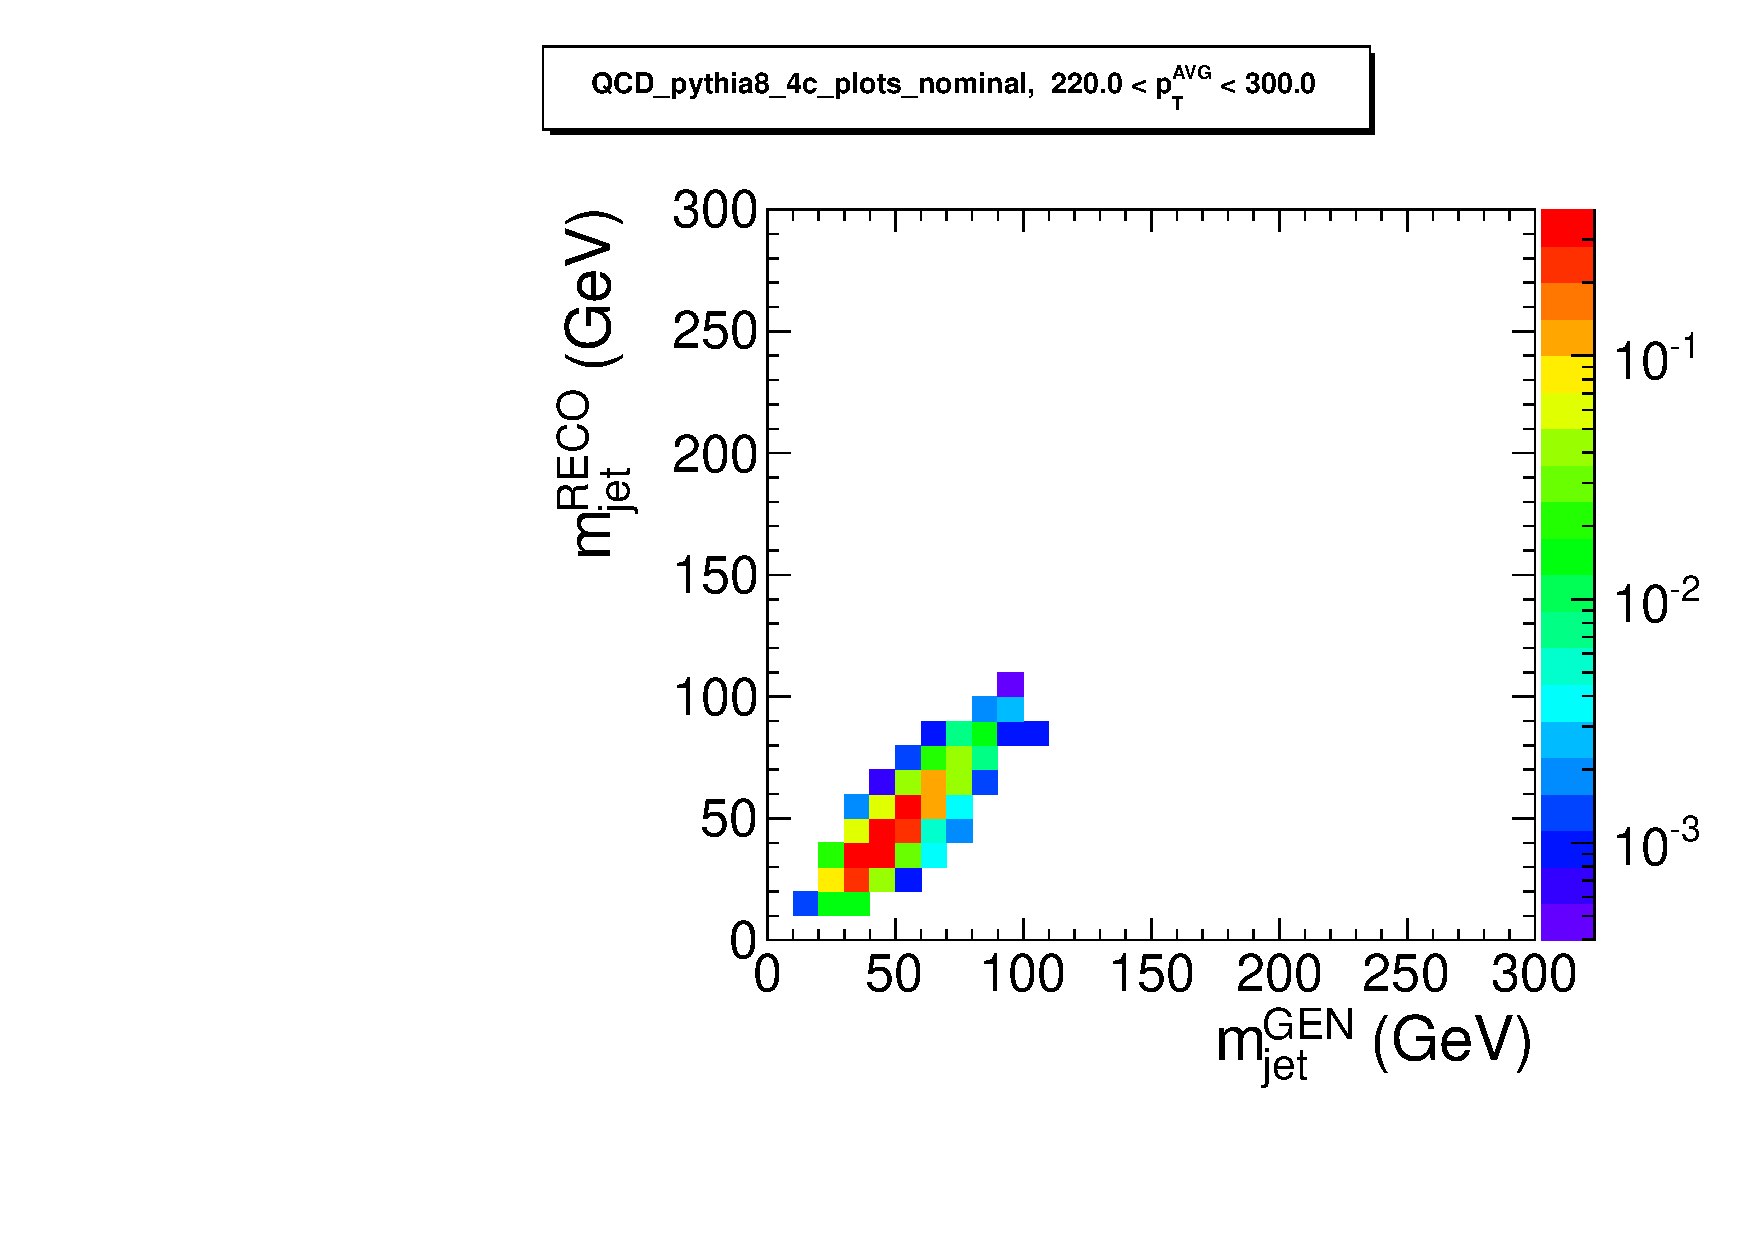
\includegraphics[width=0.3\textwidth]{figs/response_QCD_pythia8_4c_plots_nominal_pt4}}
\subfigure{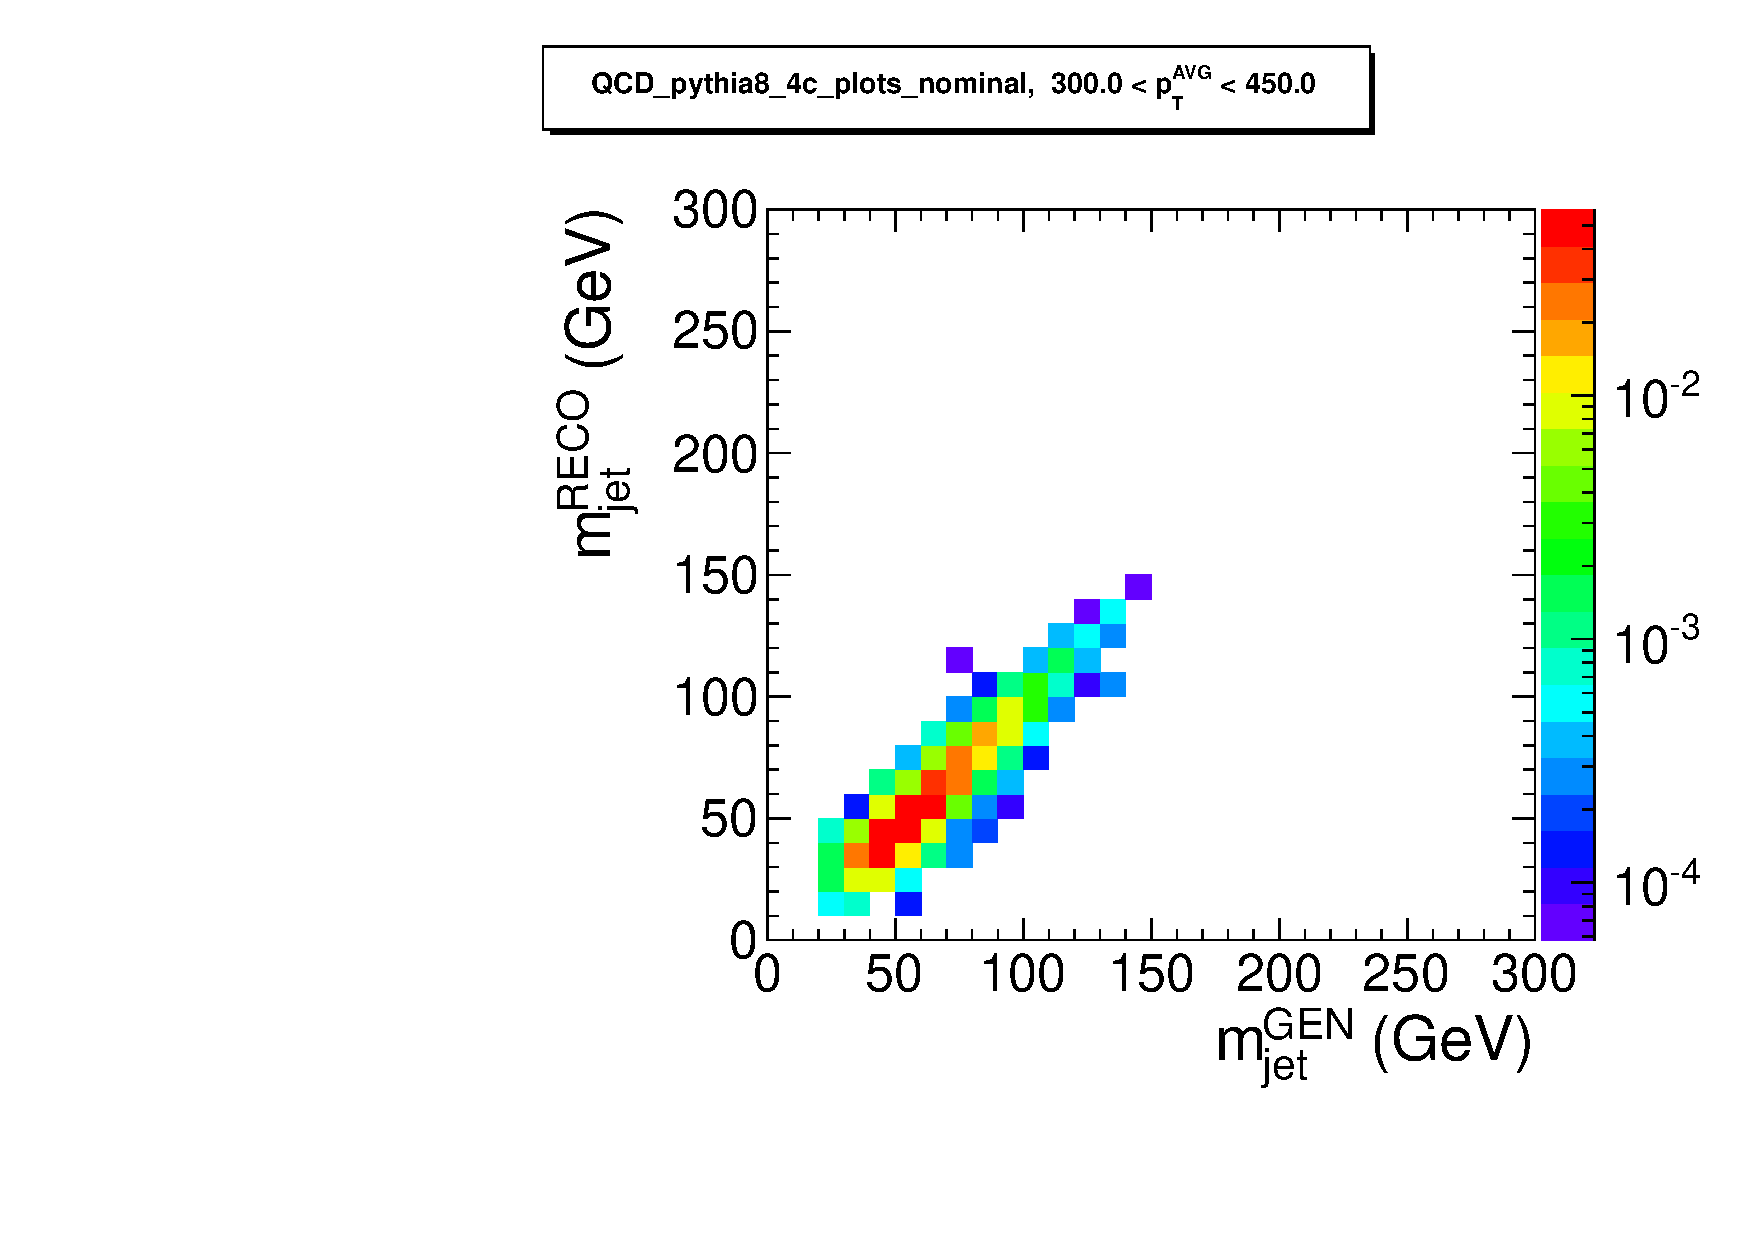
\includegraphics[width=0.3\textwidth]{figs/response_QCD_pythia8_4c_plots_nominal_pt5}}
\subfigure{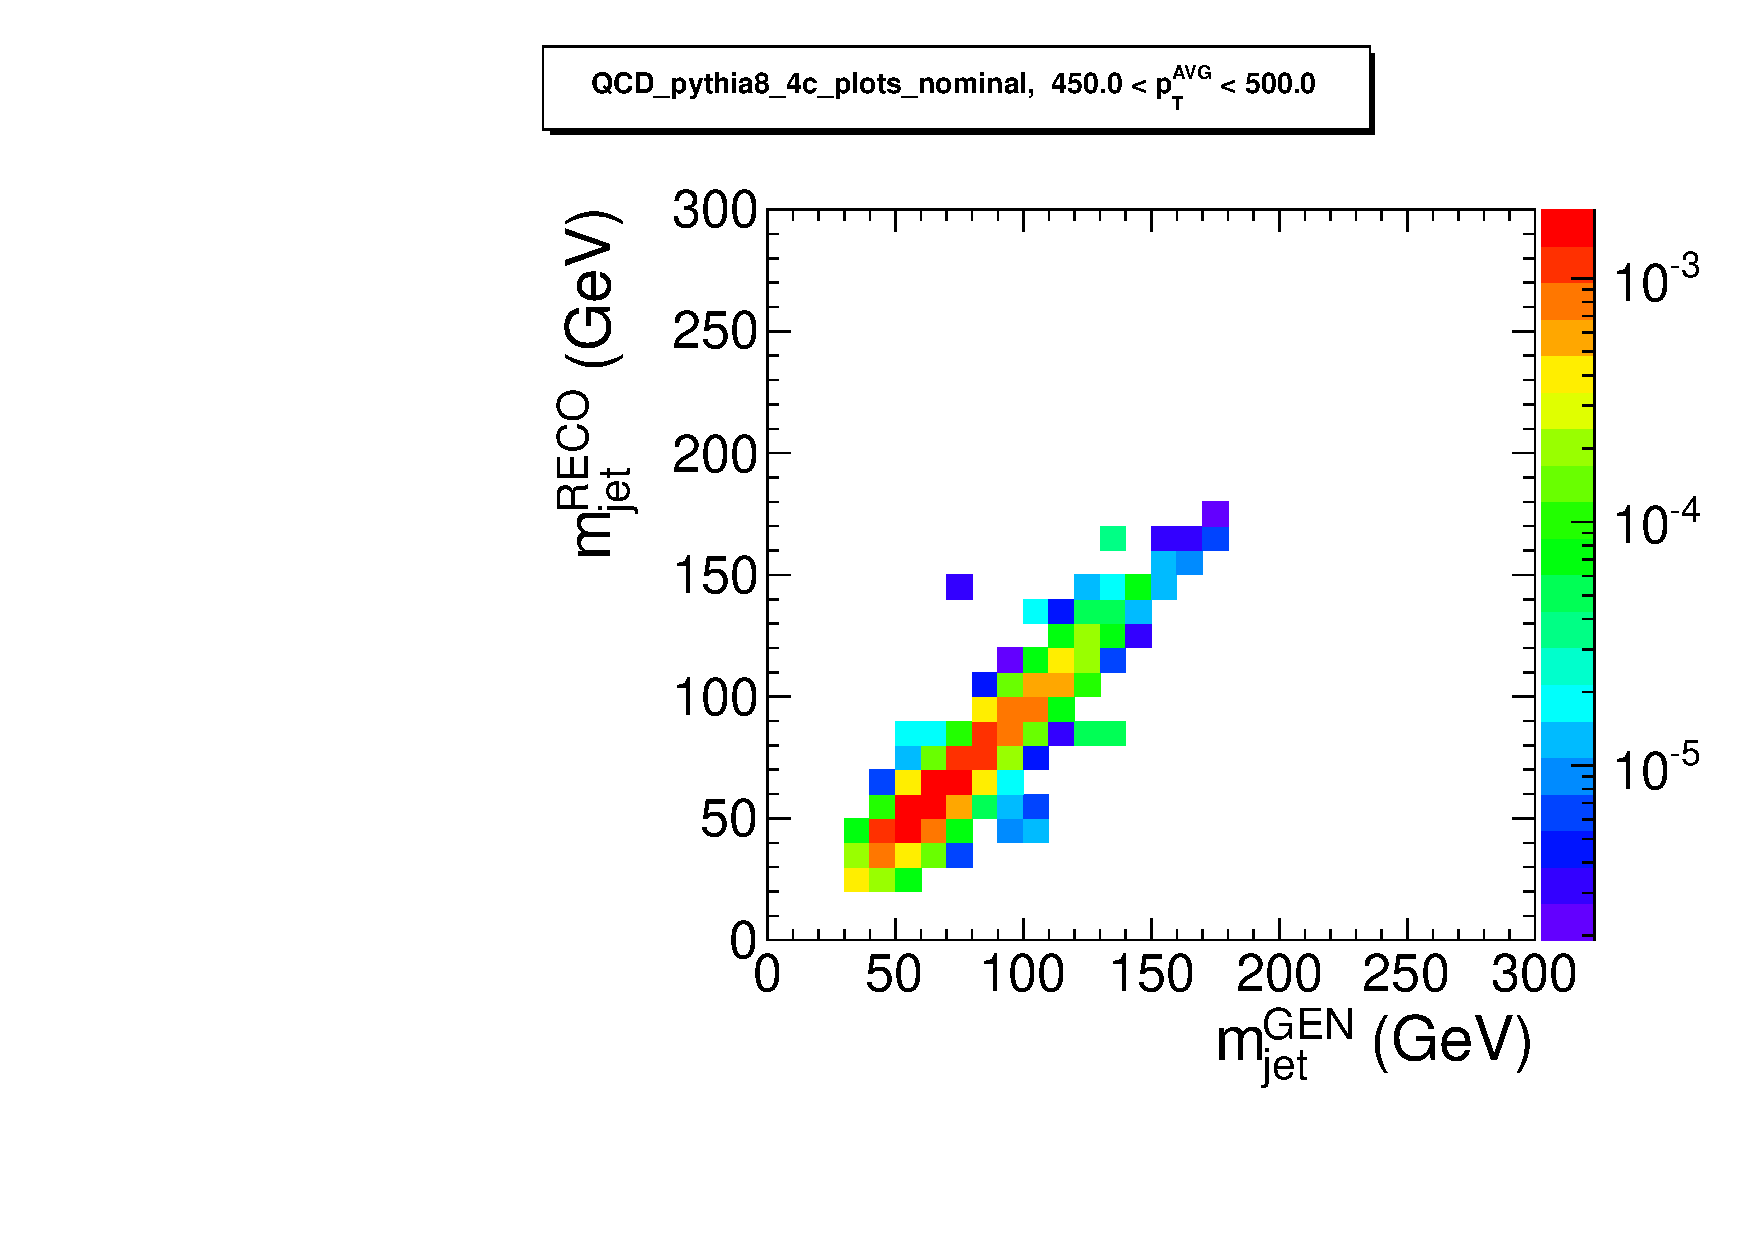
\includegraphics[width=0.3\textwidth]{figs/response_QCD_pythia8_4c_plots_nominal_pt6}}\\
\subfigure{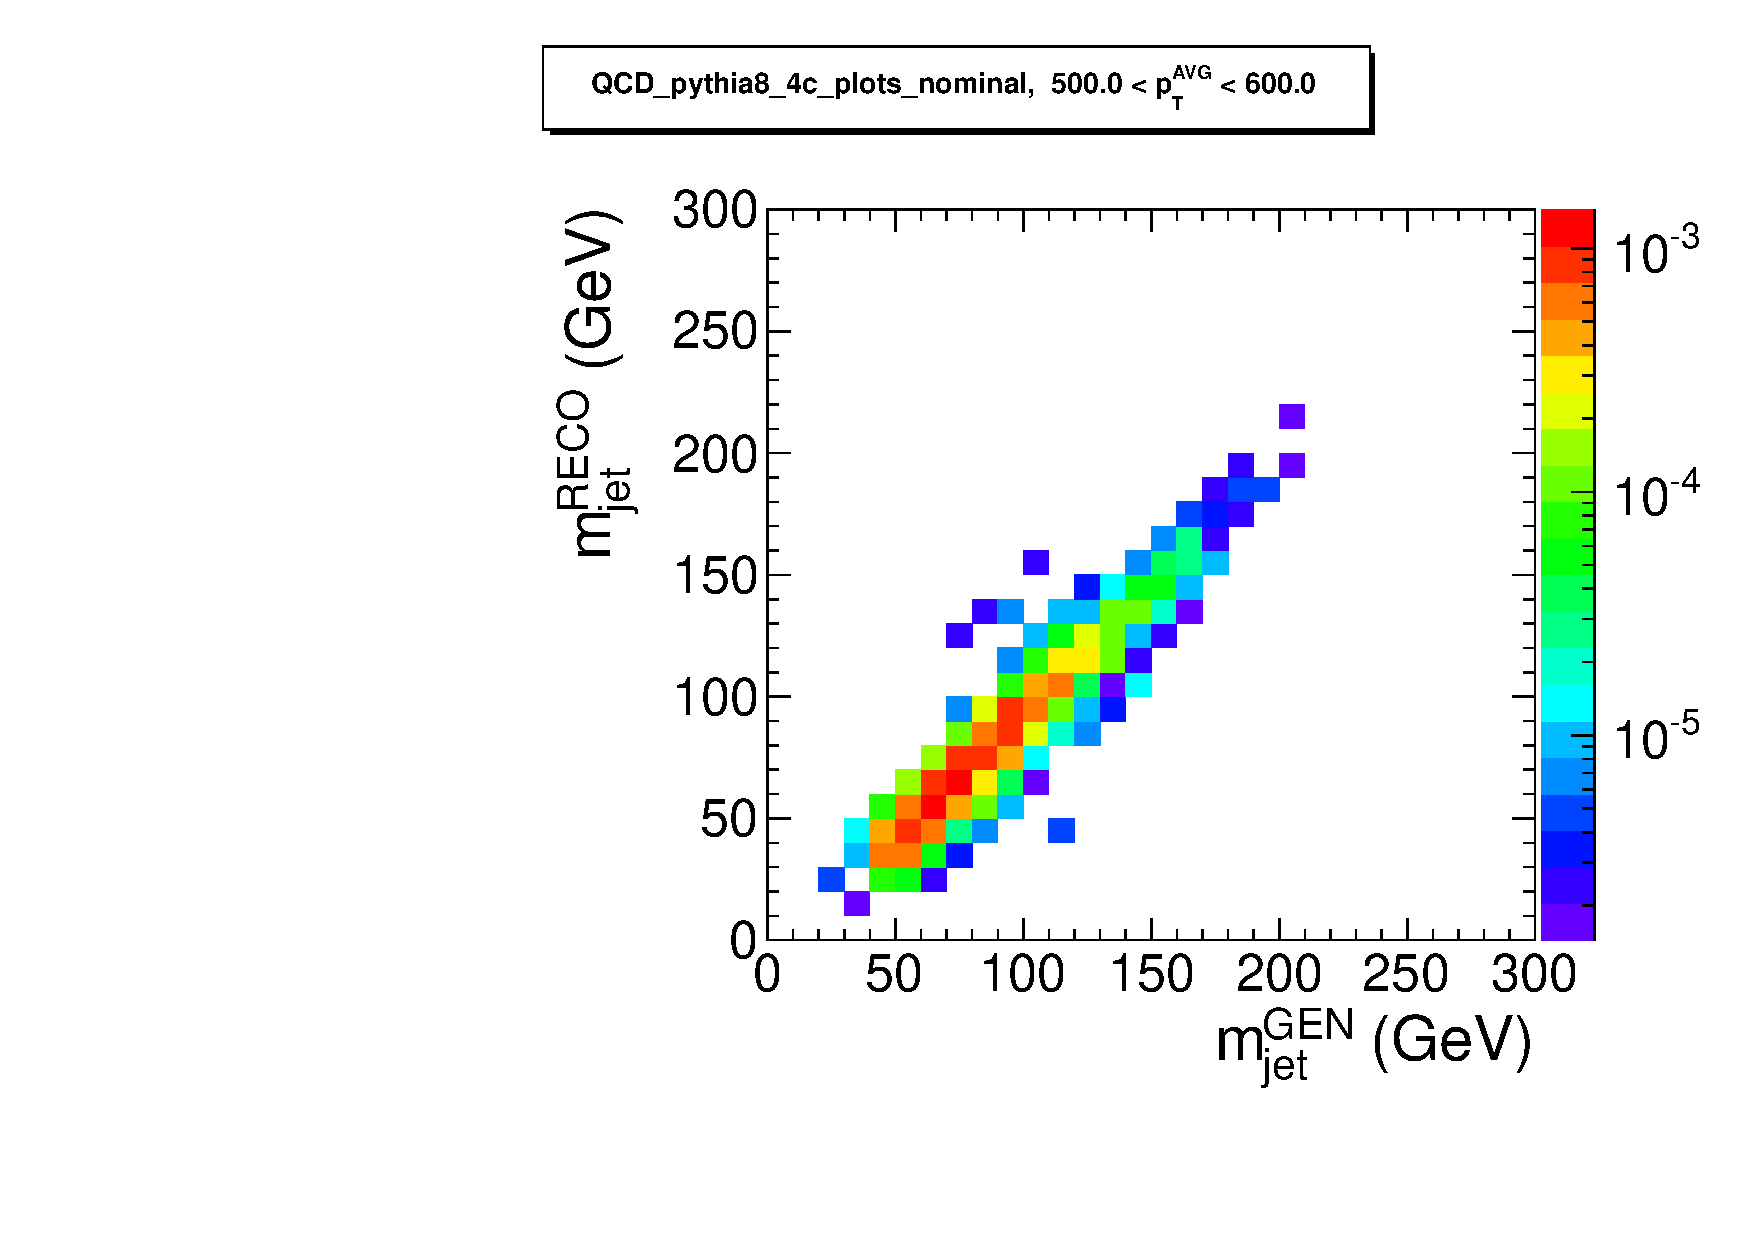
\includegraphics[width=0.3\textwidth]{figs/response_QCD_pythia8_4c_plots_nominal_pt7}}
\subfigure{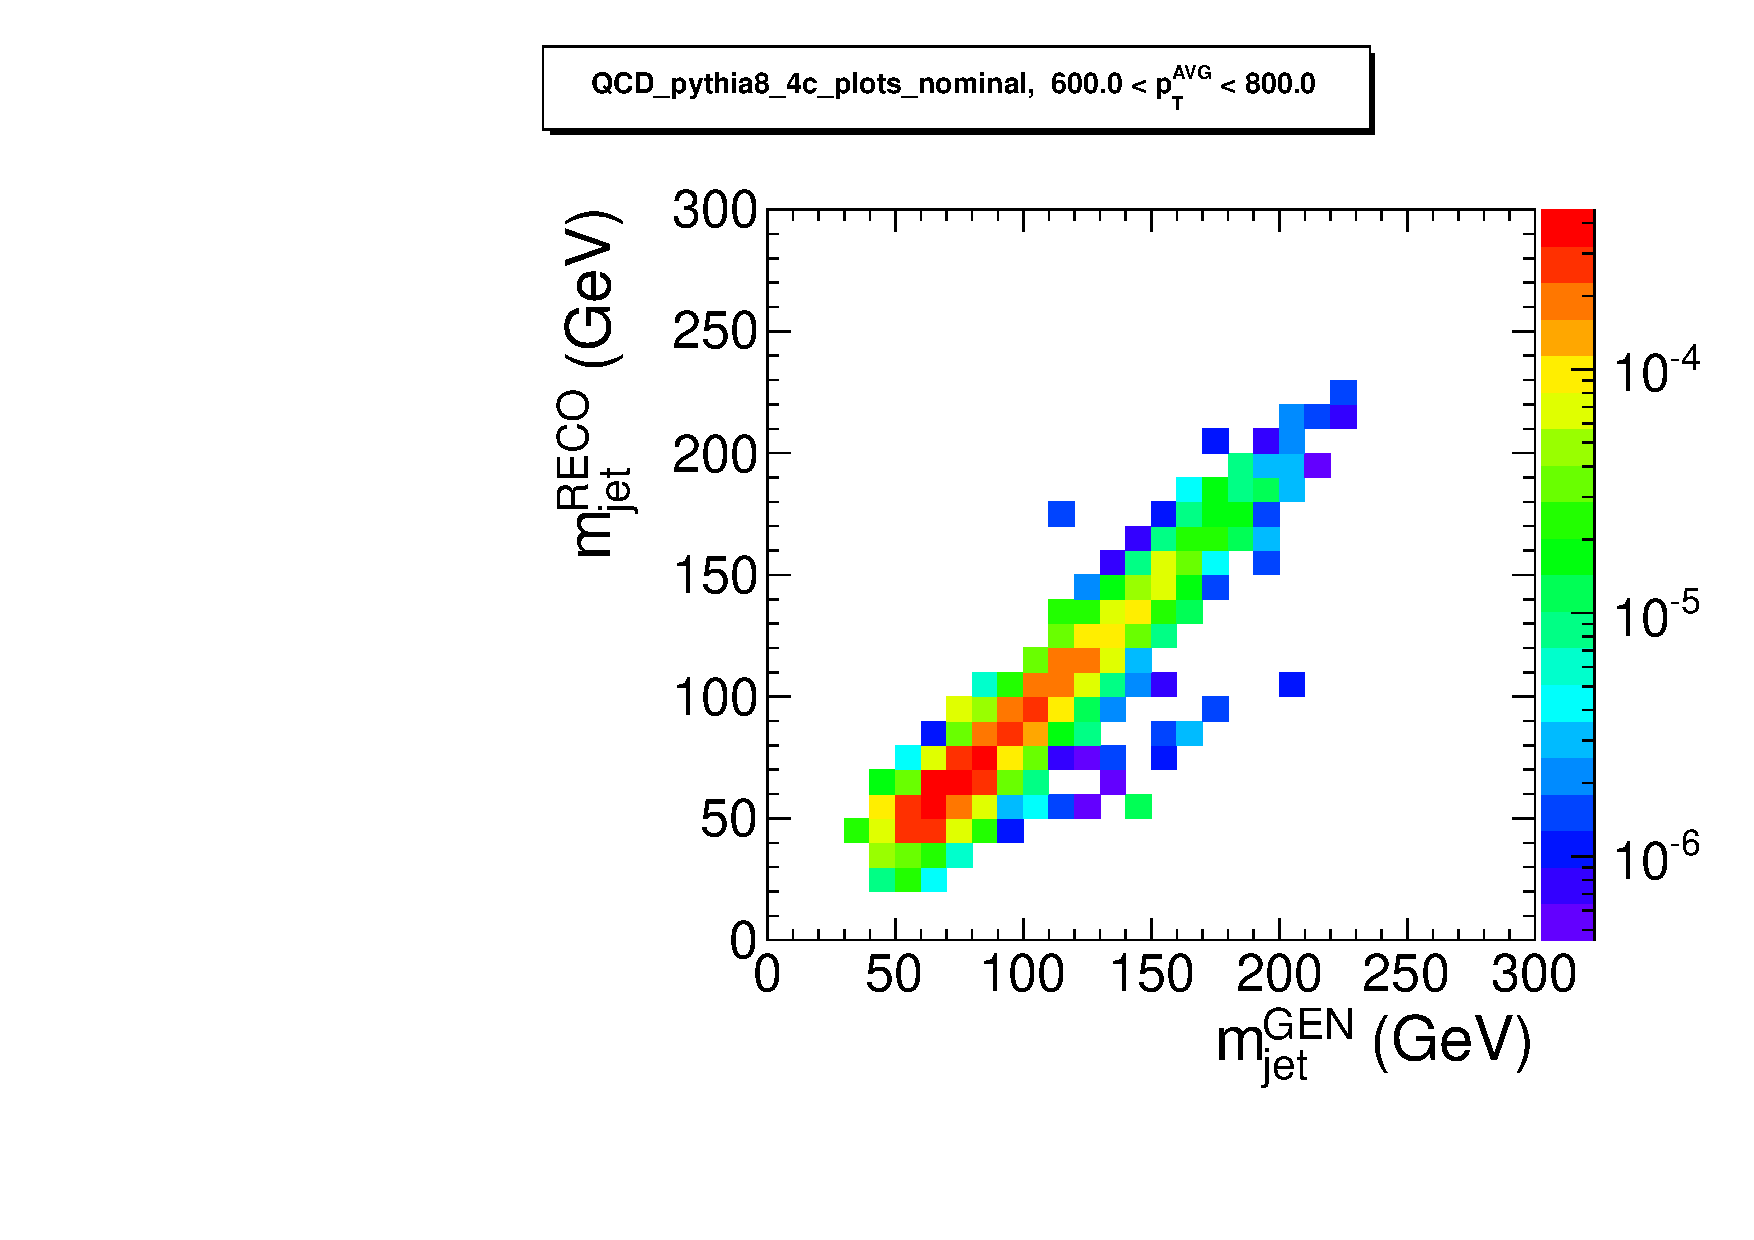
\includegraphics[width=0.3\textwidth]{figs/response_QCD_pythia8_4c_plots_nominal_pt8}}
\subfigure{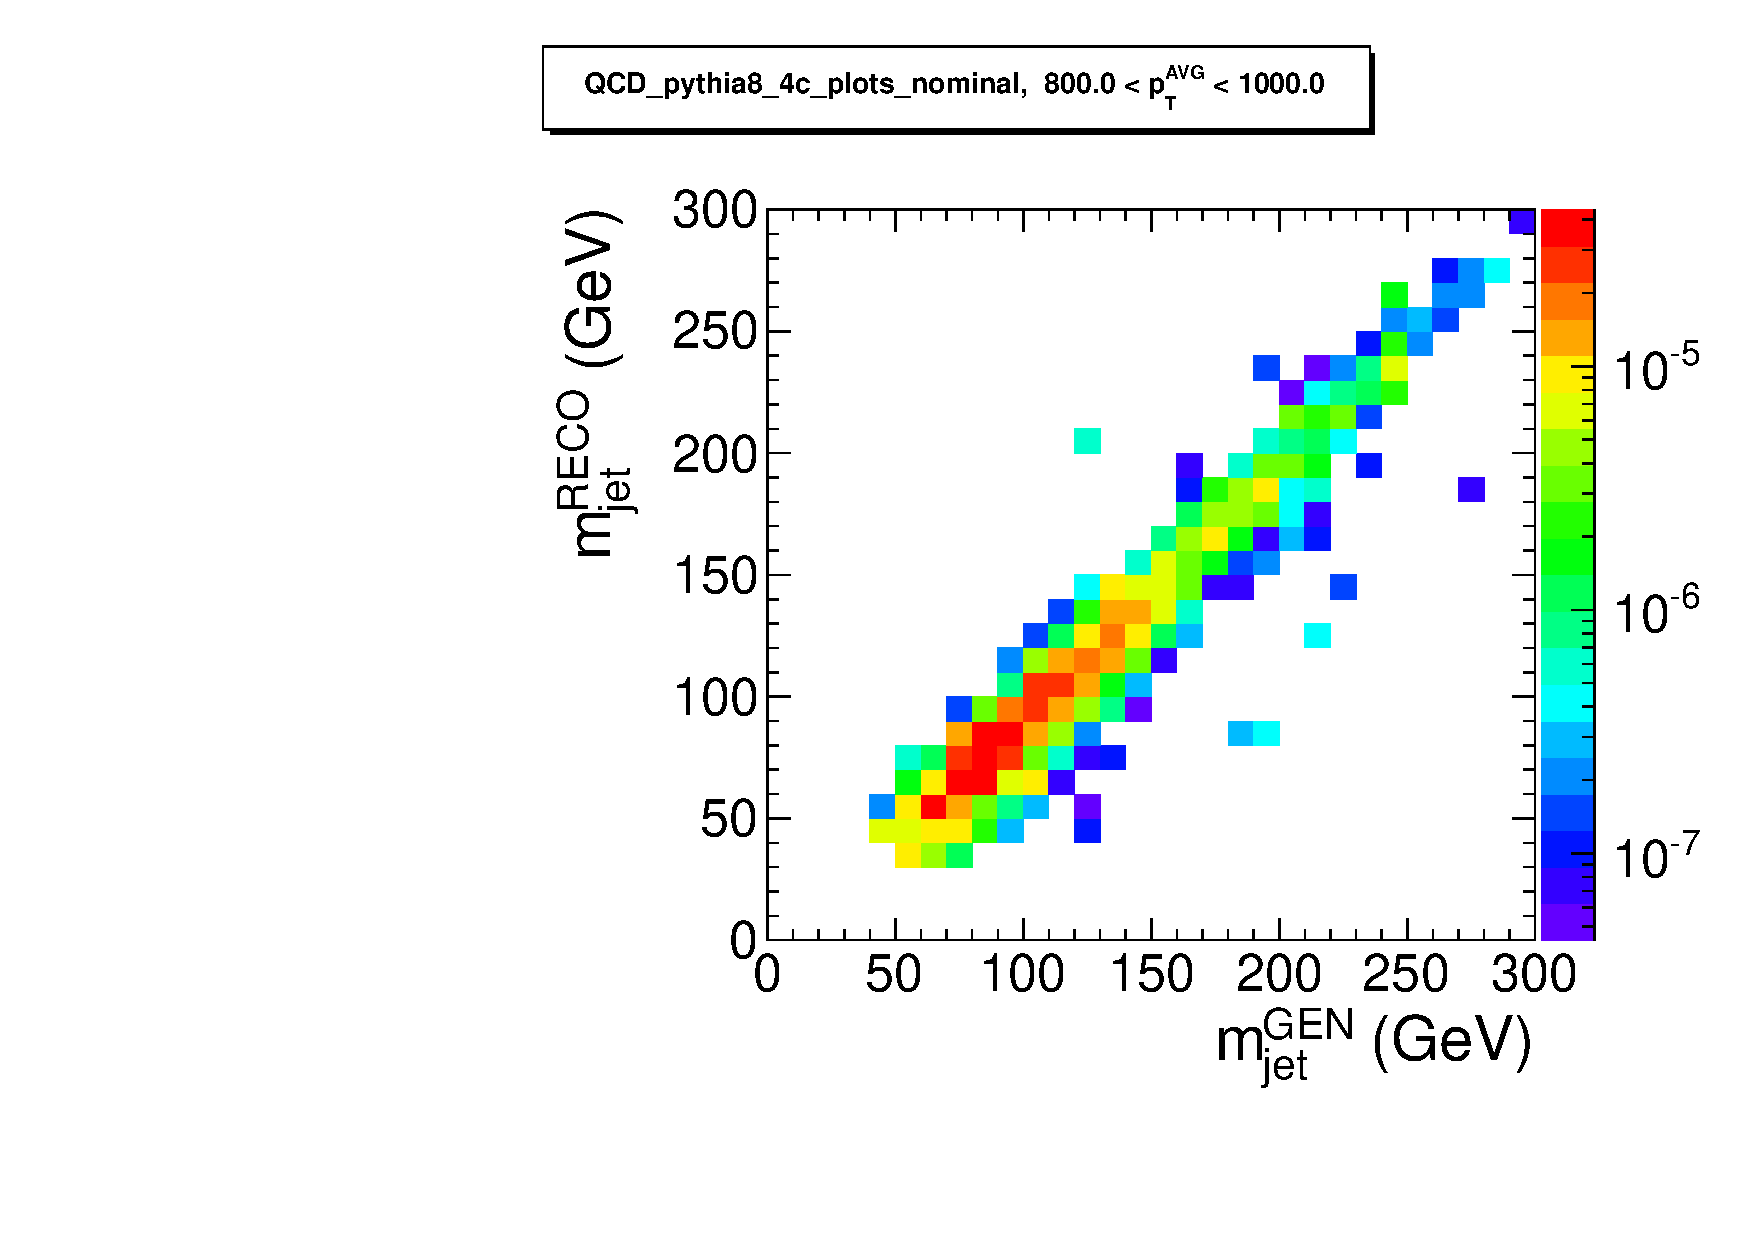
\includegraphics[width=0.3\textwidth]{figs/response_QCD_pythia8_4c_plots_nominal_pt9}}\\
\caption{Response of the jet mass for AK7 jets,
for various $\pt^{AVG}$ bins. The true jet mass is shown
on the $x-$axis, and the reconstructed jet mass is shown on the
$y-$axis, using the \PYTHIAEIGHT generator. 
\label{figs:response_QCD_pythia8_4c_plots_nominal_ptall}}
\end{figure}


\clearpage

\begin{figure}[htbp]
\centering
\subfigure{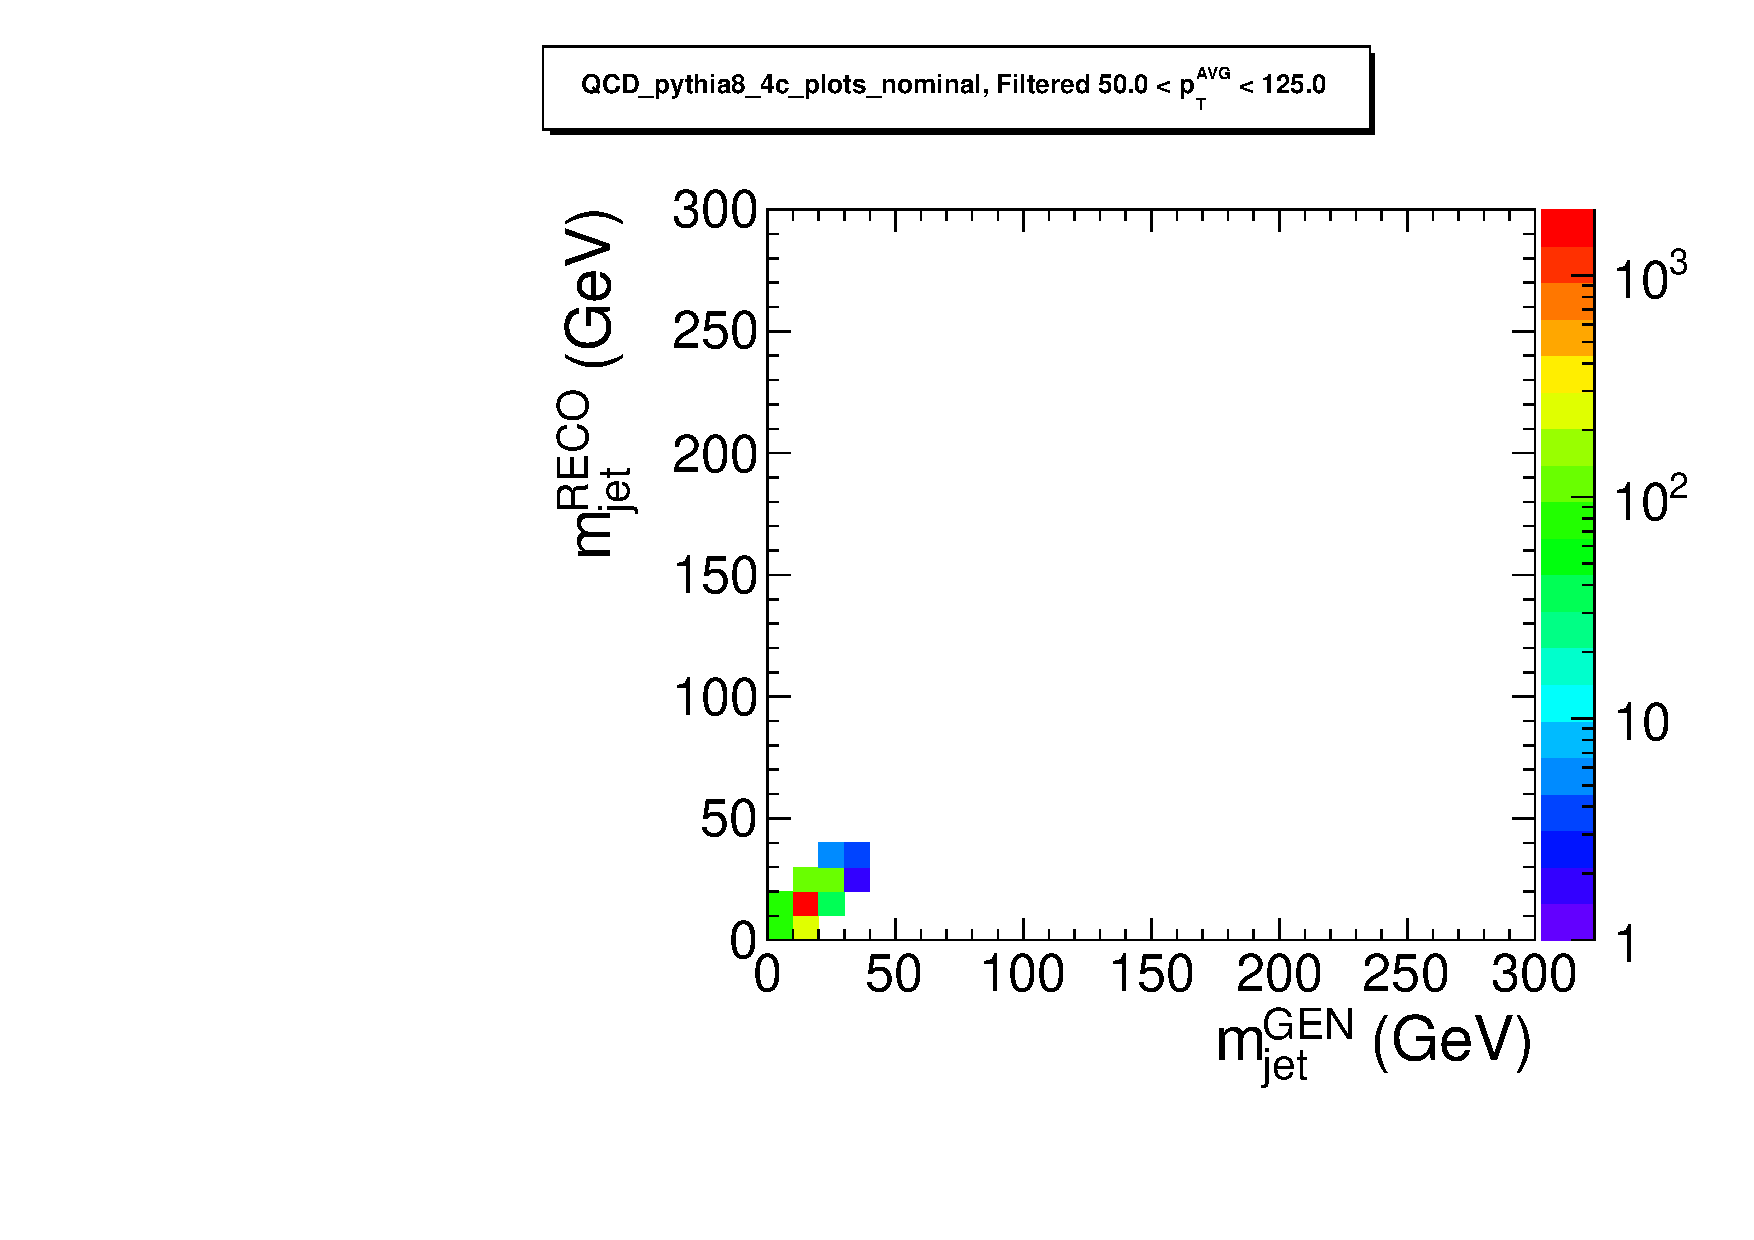
\includegraphics[width=0.3\textwidth]{figs/response_QCD_pythia8_4c_plots_nominal_Filtered_pt1}}
\subfigure{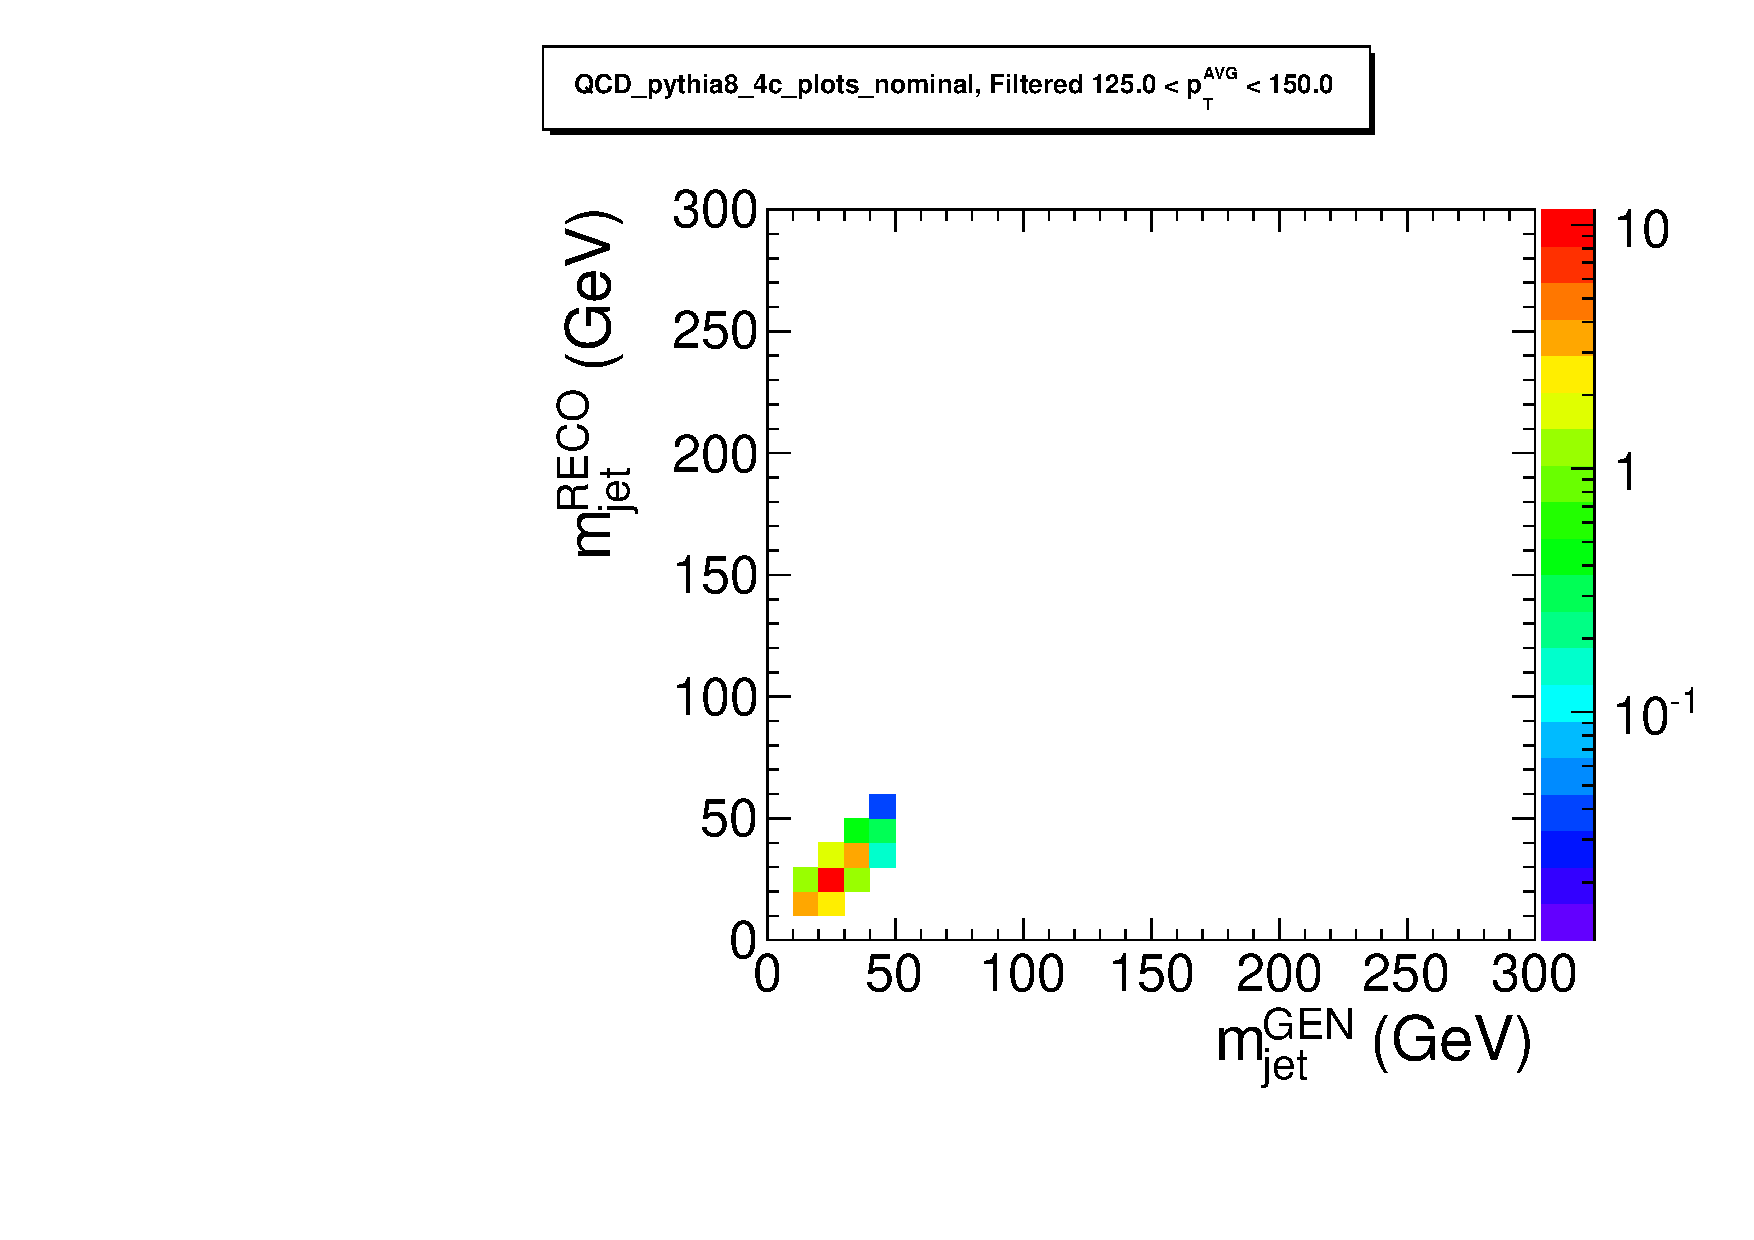
\includegraphics[width=0.3\textwidth]{figs/response_QCD_pythia8_4c_plots_nominal_Filtered_pt2}}
\subfigure{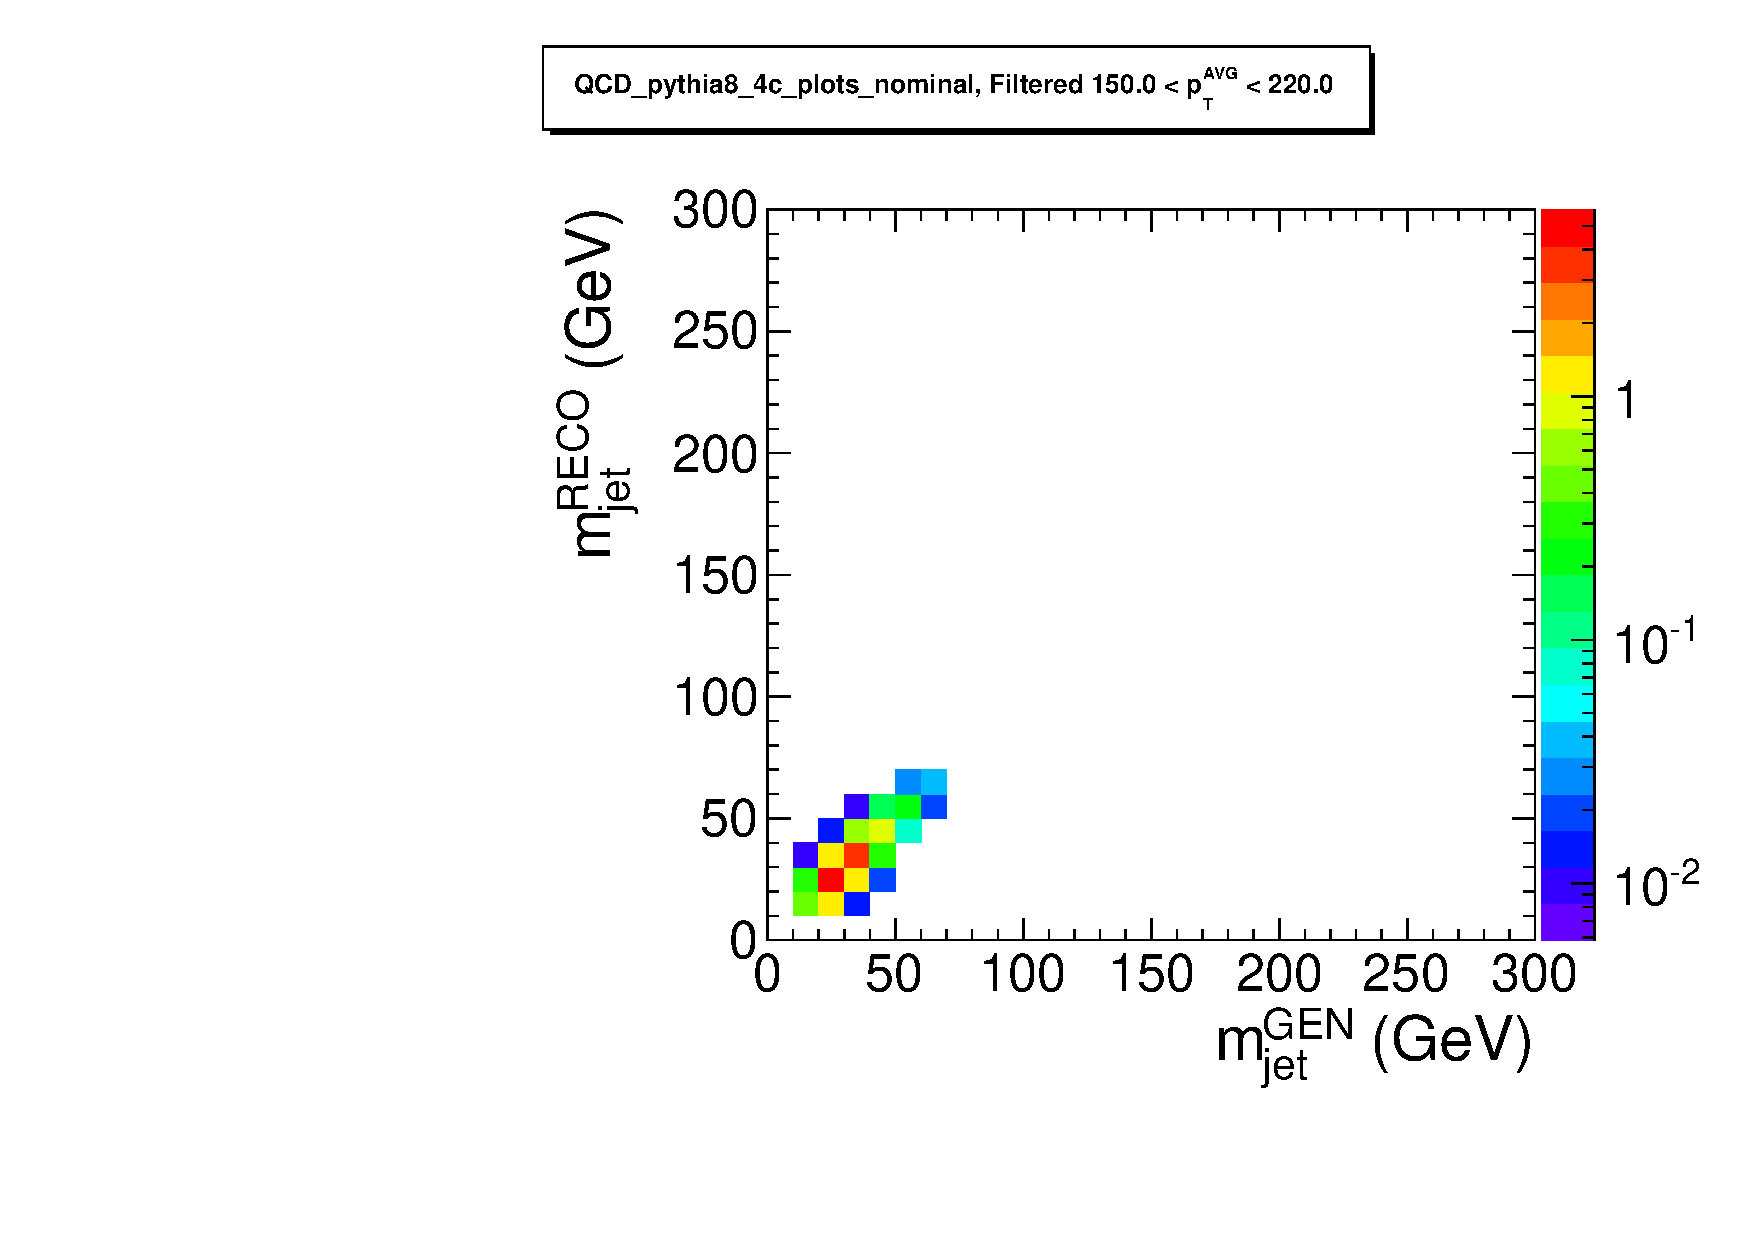
\includegraphics[width=0.3\textwidth]{figs/response_QCD_pythia8_4c_plots_nominal_Filtered_pt3}}\\
\subfigure{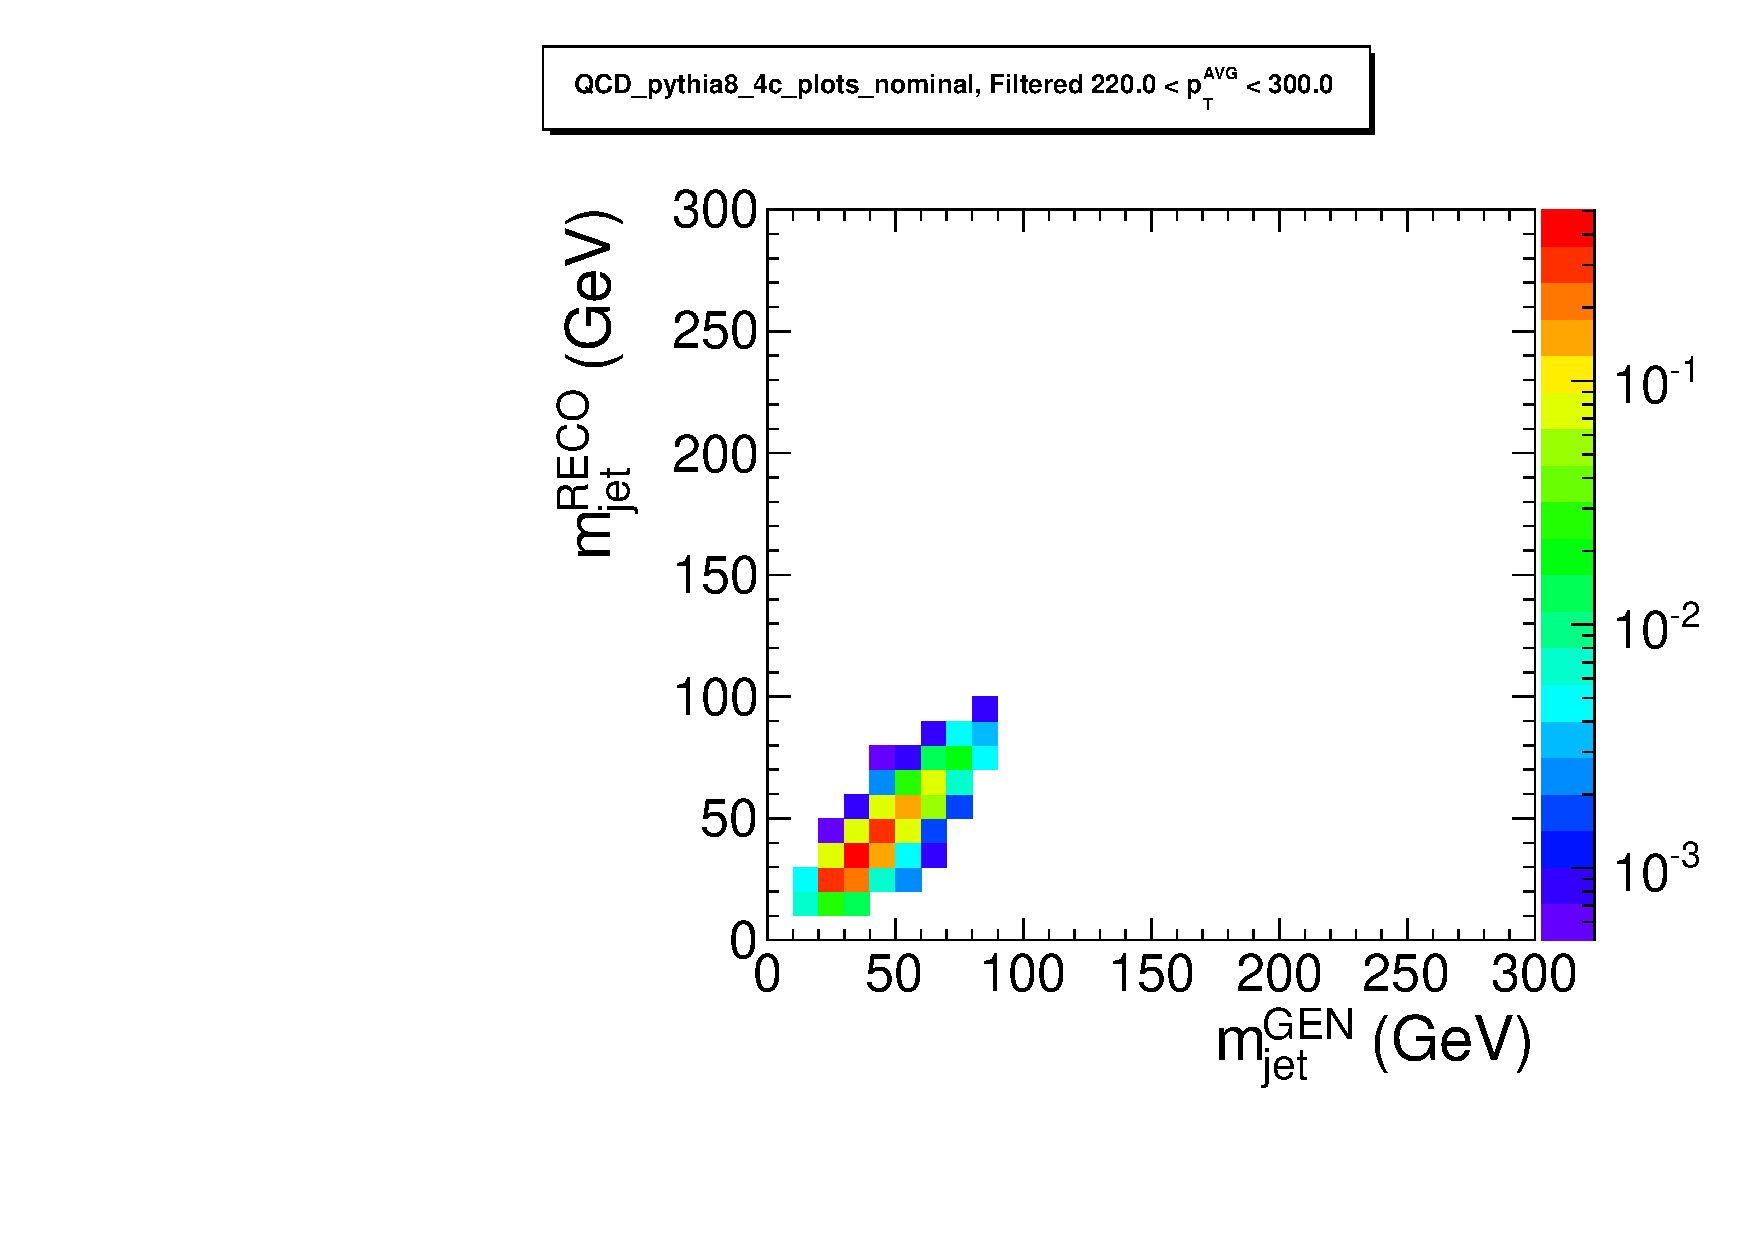
\includegraphics[width=0.3\textwidth]{figs/response_QCD_pythia8_4c_plots_nominal_Filtered_pt4}}
\subfigure{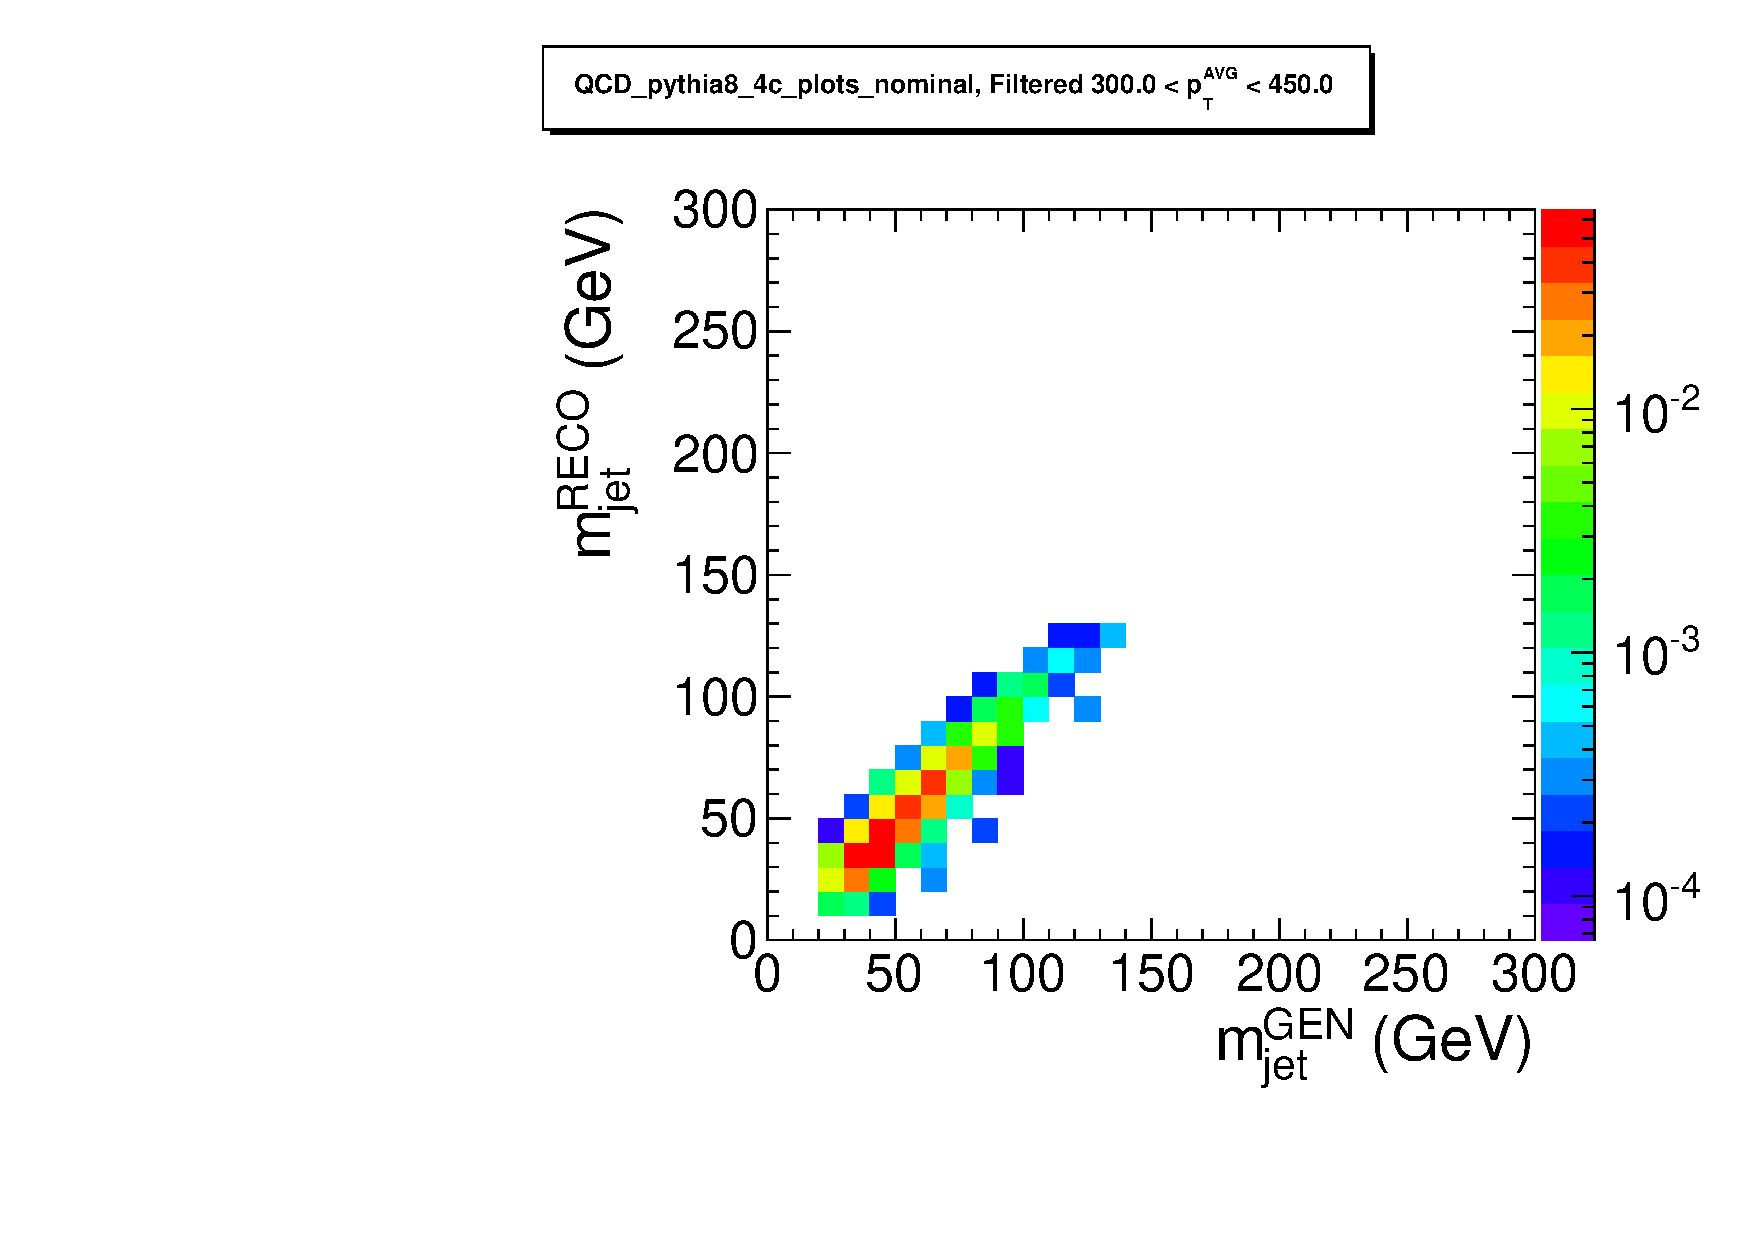
\includegraphics[width=0.3\textwidth]{figs/response_QCD_pythia8_4c_plots_nominal_Filtered_pt5}}
\subfigure{\includegraphics[width=0.3\textwidth]{figs/response_QCD_pythia8_4c_plots_nominal_Filtered_pt6}}\\
\subfigure{\includegraphics[width=0.3\textwidth]{figs/response_QCD_pythia8_4c_plots_nominal_Filtered_pt7}}
\subfigure{\includegraphics[width=0.3\textwidth]{figs/response_QCD_pythia8_4c_plots_nominal_Filtered_pt8}}
\subfigure{\includegraphics[width=0.3\textwidth]{figs/response_QCD_pythia8_4c_plots_nominal_Filtered_pt9}}\\
\caption{Response of the jet mass for AK7 Filteredjets,
for various $\pt^{AVG}$ bins. The true jet mass is shown
on the $x-$axis, and the reconstructed jet mass is shown on the
$y-$axis, using the \PYTHIAEIGHT generator. 
\label{figs:response_QCD_pythia8_4c_plots_nominal_Filtered_ptall}}
\end{figure}


\clearpage

\begin{figure}[htbp]
\centering
\subfigure{\includegraphics[width=0.3\textwidth]{figs/response_QCD_pythia8_4c_plots_nominal_Trimmed_pt1}}
\subfigure{\includegraphics[width=0.3\textwidth]{figs/response_QCD_pythia8_4c_plots_nominal_Trimmed_pt2}}
\subfigure{\includegraphics[width=0.3\textwidth]{figs/response_QCD_pythia8_4c_plots_nominal_Trimmed_pt3}}\\
\subfigure{\includegraphics[width=0.3\textwidth]{figs/response_QCD_pythia8_4c_plots_nominal_Trimmed_pt4}}
\subfigure{\includegraphics[width=0.3\textwidth]{figs/response_QCD_pythia8_4c_plots_nominal_Trimmed_pt5}}
\subfigure{\includegraphics[width=0.3\textwidth]{figs/response_QCD_pythia8_4c_plots_nominal_Trimmed_pt6}}\\
\subfigure{\includegraphics[width=0.3\textwidth]{figs/response_QCD_pythia8_4c_plots_nominal_Trimmed_pt7}}
\subfigure{\includegraphics[width=0.3\textwidth]{figs/response_QCD_pythia8_4c_plots_nominal_Trimmed_pt8}}
\subfigure{\includegraphics[width=0.3\textwidth]{figs/response_QCD_pythia8_4c_plots_nominal_Trimmed_pt9}}\\
\caption{Response of the jet mass for AK7 Trimmedjets,
for various $\pt^{AVG}$ bins. The true jet mass is shown
on the $x-$axis, and the reconstructed jet mass is shown on the
$y-$axis, using the \PYTHIAEIGHT generator. 
\label{figs:response_QCD_pythia8_4c_plots_nominal_Trimmed_ptall}}
\end{figure}


\clearpage

\begin{figure}[htbp]
\centering
\subfigure{\includegraphics[width=0.3\textwidth]{figs/response_QCD_pythia8_4c_plots_nominal_Pruned_pt1}}
\subfigure{\includegraphics[width=0.3\textwidth]{figs/response_QCD_pythia8_4c_plots_nominal_Pruned_pt2}}
\subfigure{\includegraphics[width=0.3\textwidth]{figs/response_QCD_pythia8_4c_plots_nominal_Pruned_pt3}}\\
\subfigure{\includegraphics[width=0.3\textwidth]{figs/response_QCD_pythia8_4c_plots_nominal_Pruned_pt4}}
\subfigure{\includegraphics[width=0.3\textwidth]{figs/response_QCD_pythia8_4c_plots_nominal_Pruned_pt5}}
\subfigure{\includegraphics[width=0.3\textwidth]{figs/response_QCD_pythia8_4c_plots_nominal_Pruned_pt6}}\\
\subfigure{\includegraphics[width=0.3\textwidth]{figs/response_QCD_pythia8_4c_plots_nominal_Pruned_pt7}}
\subfigure{\includegraphics[width=0.3\textwidth]{figs/response_QCD_pythia8_4c_plots_nominal_Pruned_pt8}}
\subfigure{\includegraphics[width=0.3\textwidth]{figs/response_QCD_pythia8_4c_plots_nominal_Pruned_pt9}}\\
\caption{Response of the jet mass for AK7 Prunedjets,
for various $\pt^{AVG}$ bins. The true jet mass is shown
on the $x-$axis, and the reconstructed jet mass is shown on the
$y-$axis, using the \PYTHIAEIGHT generator. 
\label{figs:response_QCD_pythia8_4c_plots_nominal_Pruned_ptall}}
\end{figure}


\clearpage

\begin{figure}[htbp]
\centering
\subfigure{\includegraphics[width=0.3\textwidth]{figs/response_QCD_herwigpp_23_plots_nominal_pt1}}
\subfigure{\includegraphics[width=0.3\textwidth]{figs/response_QCD_herwigpp_23_plots_nominal_pt2}}
\subfigure{\includegraphics[width=0.3\textwidth]{figs/response_QCD_herwigpp_23_plots_nominal_pt3}}\\
\subfigure{\includegraphics[width=0.3\textwidth]{figs/response_QCD_herwigpp_23_plots_nominal_pt4}}
\subfigure{\includegraphics[width=0.3\textwidth]{figs/response_QCD_herwigpp_23_plots_nominal_pt5}}
\subfigure{\includegraphics[width=0.3\textwidth]{figs/response_QCD_herwigpp_23_plots_nominal_pt6}}\\
\subfigure{\includegraphics[width=0.3\textwidth]{figs/response_QCD_herwigpp_23_plots_nominal_pt7}}
\subfigure{\includegraphics[width=0.3\textwidth]{figs/response_QCD_herwigpp_23_plots_nominal_pt8}}
\subfigure{\includegraphics[width=0.3\textwidth]{figs/response_QCD_herwigpp_23_plots_nominal_pt9}}\\
\caption{Response of the jet mass for AK7 jets,
for various $\pt^{AVG}$ bins. The true jet mass is shown
on the $x-$axis, and the reconstructed jet mass is shown on the
$y-$axis, using the \HERWIG generator. 
\label{figs:response_QCD_herwigpp_23_plots_nominal_ptall}}
\end{figure}


\clearpage

\begin{figure}[htbp]
\centering
\subfigure{\includegraphics[width=0.3\textwidth]{figs/response_QCD_herwigpp_23_plots_nominal_Filtered_pt1}}
\subfigure{\includegraphics[width=0.3\textwidth]{figs/response_QCD_herwigpp_23_plots_nominal_Filtered_pt2}}
\subfigure{\includegraphics[width=0.3\textwidth]{figs/response_QCD_herwigpp_23_plots_nominal_Filtered_pt3}}\\
\subfigure{\includegraphics[width=0.3\textwidth]{figs/response_QCD_herwigpp_23_plots_nominal_Filtered_pt4}}
\subfigure{\includegraphics[width=0.3\textwidth]{figs/response_QCD_herwigpp_23_plots_nominal_Filtered_pt5}}
\subfigure{\includegraphics[width=0.3\textwidth]{figs/response_QCD_herwigpp_23_plots_nominal_Filtered_pt6}}\\
\subfigure{\includegraphics[width=0.3\textwidth]{figs/response_QCD_herwigpp_23_plots_nominal_Filtered_pt7}}
\subfigure{\includegraphics[width=0.3\textwidth]{figs/response_QCD_herwigpp_23_plots_nominal_Filtered_pt8}}
\subfigure{\includegraphics[width=0.3\textwidth]{figs/response_QCD_herwigpp_23_plots_nominal_Filtered_pt9}}\\
\caption{Response of the jet mass for AK7 Filteredjets,
for various $\pt^{AVG}$ bins. The true jet mass is shown
on the $x-$axis, and the reconstructed jet mass is shown on the
$y-$axis, using the \HERWIG generator. 
\label{figs:response_QCD_herwigpp_23_plots_nominal_Filtered_ptall}}
\end{figure}


\clearpage

\begin{figure}[htbp]
\centering
\subfigure{\includegraphics[width=0.3\textwidth]{figs/response_QCD_herwigpp_23_plots_nominal_Trimmed_pt1}}
\subfigure{\includegraphics[width=0.3\textwidth]{figs/response_QCD_herwigpp_23_plots_nominal_Trimmed_pt2}}
\subfigure{\includegraphics[width=0.3\textwidth]{figs/response_QCD_herwigpp_23_plots_nominal_Trimmed_pt3}}\\
\subfigure{\includegraphics[width=0.3\textwidth]{figs/response_QCD_herwigpp_23_plots_nominal_Trimmed_pt4}}
\subfigure{\includegraphics[width=0.3\textwidth]{figs/response_QCD_herwigpp_23_plots_nominal_Trimmed_pt5}}
\subfigure{\includegraphics[width=0.3\textwidth]{figs/response_QCD_herwigpp_23_plots_nominal_Trimmed_pt6}}\\
\subfigure{\includegraphics[width=0.3\textwidth]{figs/response_QCD_herwigpp_23_plots_nominal_Trimmed_pt7}}
\subfigure{\includegraphics[width=0.3\textwidth]{figs/response_QCD_herwigpp_23_plots_nominal_Trimmed_pt8}}
\subfigure{\includegraphics[width=0.3\textwidth]{figs/response_QCD_herwigpp_23_plots_nominal_Trimmed_pt9}}\\
\caption{Response of the jet mass for AK7 Trimmedjets,
for various $\pt^{AVG}$ bins. The true jet mass is shown
on the $x-$axis, and the reconstructed jet mass is shown on the
$y-$axis, using the \HERWIG generator. 
\label{figs:response_QCD_herwigpp_23_plots_nominal_Trimmed_ptall}}
\end{figure}


\clearpage

\begin{figure}[htbp]
\centering
\subfigure{\includegraphics[width=0.3\textwidth]{figs/response_QCD_herwigpp_23_plots_nominal_Pruned_pt1}}
\subfigure{\includegraphics[width=0.3\textwidth]{figs/response_QCD_herwigpp_23_plots_nominal_Pruned_pt2}}
\subfigure{\includegraphics[width=0.3\textwidth]{figs/response_QCD_herwigpp_23_plots_nominal_Pruned_pt3}}\\
\subfigure{\includegraphics[width=0.3\textwidth]{figs/response_QCD_herwigpp_23_plots_nominal_Pruned_pt4}}
\subfigure{\includegraphics[width=0.3\textwidth]{figs/response_QCD_herwigpp_23_plots_nominal_Pruned_pt5}}
\subfigure{\includegraphics[width=0.3\textwidth]{figs/response_QCD_herwigpp_23_plots_nominal_Pruned_pt6}}\\
\subfigure{\includegraphics[width=0.3\textwidth]{figs/response_QCD_herwigpp_23_plots_nominal_Pruned_pt7}}
\subfigure{\includegraphics[width=0.3\textwidth]{figs/response_QCD_herwigpp_23_plots_nominal_Pruned_pt8}}
\subfigure{\includegraphics[width=0.3\textwidth]{figs/response_QCD_herwigpp_23_plots_nominal_Pruned_pt9}}\\
\caption{Response of the jet mass for AK7 Prunedjets,
for various $\pt^{AVG}$ bins. The true jet mass is shown
on the $x-$axis, and the reconstructed jet mass is shown on the
$y-$axis, using the \HERWIG generator. 
\label{figs:response_QCD_herwigpp_23_plots_nominal_Pruned_ptall}}
\end{figure}


\clearpage


\clearpage

\subsection{Closure test}

\label{sec:closure}

The unfolding procedure we have used makes an assumption that
the dijet events that we are using are the same at the detector
level and the generator level. Furthermore, the jet algorithm
itself is an arbitrary designation of the event, and what to
call a ``jet'' depends on the energy scale of the process.
For these reasons, the assumed dijet topology as described
above may not correspond to the true topology of the event.
Trijet events (and quadjet, etc) can pollute the dijet
events, even with a veto on extra jet activity. This is 
particularly problematic at lower $\pt$. Hence, a critical test
is the closure of our unfolding procedure. That is,
the MC is taken as both the input to the response matrix,
and as simulated ``data'', and compared to the MC true
distribution at the generator level. Any discrepancy here
is a problem with the assumption of the dijet topology.

Figures~\ref{figs:unfoldedMeasurementDijets_1_closuretest}-
\ref{figs:unfoldedMeasurementDijets_9_closuretest}
show the closure test for the various $\pt^{AVG}$ bins
in the sample. Here, the \PYTHIA true distributions
are compared against the unfolded \PYTHIA MC distributions,
using the unfolding matrix derived from \PYTHIA. For perfect
closure, all of the bins will be at unity. 

There are some residual biases that are present for the 
lower ${\pt}^{AVG}$ bins. These are explicitly corrected
in the unfolded distributions, and the correction is
taken as a systematic uncertainty. 

\begin{figure}[htbp]
\centering
\includegraphics[width=0.95\textwidth]{figs/unfoldedMeasurementDijets_1_closuretest}
\caption{Closure test of the unfolding procedure of the jet mass for AK7 jets,
for $50.0 < \pt^{AVG} < 125.0$ \GeVc. The unfolded MC distribution is shown in black points.
The true MC distribution is shown in solid black. For perfect closure, the black points would
lie exactly on the solid black line.  
\label{figs:unfoldedMeasurementDijets_1_closuretest}}
\end{figure}



\begin{figure}[htbp]
\centering
\includegraphics[width=0.95\textwidth]{figs/unfoldedMeasurementDijets_2_closuretest}
\caption{Closure test of the unfolding procedure of the jet mass for AK7 jets,
for $125.0 < \pt^{AVG} < 150.0$ \GeVc. The unfolded MC distribution is shown in black points.
The true MC distribution is shown in solid black. For perfect closure, the black points would
lie exactly on the solid black line.  
\label{figs:unfoldedMeasurementDijets_2_closuretest}}
\end{figure}



\begin{figure}[htbp]
\centering
\includegraphics[width=0.95\textwidth]{figs/unfoldedMeasurementDijets_3_closuretest}
\caption{Closure test of the unfolding procedure of the jet mass for AK7 jets,
for $150.0 < \pt^{AVG} < 220.0$ \GeVc. The unfolded MC distribution is shown in black points.
The true MC distribution is shown in solid black. For perfect closure, the black points would
lie exactly on the solid black line.  
\label{figs:unfoldedMeasurementDijets_3_closuretest}}
\end{figure}



\begin{figure}[htbp]
\centering
\includegraphics[width=0.95\textwidth]{figs/unfoldedMeasurementDijets_4_closuretest}
\caption{Closure test of the unfolding procedure of the jet mass for AK7 jets,
for $220.0 < \pt^{AVG} < 300.0$ \GeVc. The unfolded MC distribution is shown in black points.
The true MC distribution is shown in solid black. For perfect closure, the black points would
lie exactly on the solid black line.  
\label{figs:unfoldedMeasurementDijets_4_closuretest}}
\end{figure}



\begin{figure}[htbp]
\centering
\includegraphics[width=0.95\textwidth]{figs/unfoldedMeasurementDijets_5_closuretest}
\caption{Closure test of the unfolding procedure of the jet mass for AK7 jets,
for $300.0 < \pt^{AVG} < 450.0$ \GeVc. The unfolded MC distribution is shown in black points.
The true MC distribution is shown in solid black. For perfect closure, the black points would
lie exactly on the solid black line.  
\label{figs:unfoldedMeasurementDijets_5_closuretest}}
\end{figure}



\begin{figure}[htbp]
\centering
\includegraphics[width=0.95\textwidth]{figs/unfoldedMeasurementDijets_6_closuretest}
\caption{Closure test of the unfolding procedure of the jet mass for AK7 jets,
for $450.0 < \pt^{AVG} < 500.0$ \GeVc. The unfolded MC distribution is shown in black points.
The true MC distribution is shown in solid black. For perfect closure, the black points would
lie exactly on the solid black line.  
\label{figs:unfoldedMeasurementDijets_6_closuretest}}
\end{figure}



\begin{figure}[htbp]
\centering
\includegraphics[width=0.95\textwidth]{figs/unfoldedMeasurementDijets_7_closuretest}
\caption{Closure test of the unfolding procedure of the jet mass for AK7 jets,
for $500.0 < \pt^{AVG} < 600.0$ \GeVc. The unfolded MC distribution is shown in black points.
The true MC distribution is shown in solid black. For perfect closure, the black points would
lie exactly on the solid black line.  
\label{figs:unfoldedMeasurementDijets_7_closuretest}}
\end{figure}



\begin{figure}[htbp]
\centering
\includegraphics[width=0.95\textwidth]{figs/unfoldedMeasurementDijets_8_closuretest}
\caption{Closure test of the unfolding procedure of the jet mass for AK7 jets,
for $600.0 < \pt^{AVG} < 800.0$ \GeVc. The unfolded MC distribution is shown in black points.
The true MC distribution is shown in solid black. For perfect closure, the black points would
lie exactly on the solid black line.  
\label{figs:unfoldedMeasurementDijets_8_closuretest}}
\end{figure}



\begin{figure}[htbp]
\centering
\includegraphics[width=0.95\textwidth]{figs/unfoldedMeasurementDijets_9_closuretest}
\caption{Closure test of the unfolding procedure of the jet mass for AK7 jets,
for $800.0 < \pt^{AVG} < 1000.0$ \GeVc. The unfolded MC distribution is shown in black points.
The true MC distribution is shown in solid black. For perfect closure, the black points would
lie exactly on the solid black line.  
\label{figs:unfoldedMeasurementDijets_9_closuretest}}
\end{figure}



\begin{figure}[htbp]
\centering
\includegraphics[width=0.95\textwidth]{figs/unfoldedMeasurementDijets_10_closuretest}
\caption{Closure test of the unfolding procedure of the jet mass for AK7 jets,
for $1000.0 < \pt^{AVG} < 1500.0$ \GeVc. The unfolded MC distribution is shown in black points.
The true MC distribution is shown in solid black. For perfect closure, the black points would
lie exactly on the solid black line.  
\label{figs:unfoldedMeasurementDijets_10_closuretest}}
\end{figure}

\clearpage


